\begin{talk}
  {New error estimates for the Adam optimization algorithm}% [1] talk title
  {Steffen Dereich}% [2] speaker name
  {University of M\"unster}% [3] affiliations
  {steffen.dereich@uni-muenster.de}% [4] email
  {Arnulf Jentzen}% [5] coauthors
{}{\timeslot{Monday, August 19, 2024 -- Morning}{STC 0020}}{SS3-2}{SS3}

				% Insert the title of the special session if you were invited to give a talk in a special session.
			
%Your abstract goes here. Please do not use your own commands or macros.

The Adam optimization algorithm is a very popular training algorithm for artificial neural networks. It is a stochastic gradient descent algorithm that combines a momentum approach with a damping factor. Despite its popularity its theoretical analysis is still in its infancy. In this talk, we provide new error estimates for the Adam algorithm and we illustrate our findings in a simple example, where we estimate expectations of random variables.

\end{talk}

\begin{talk}
  {Upper and Lower Bounds for Pathwise Approximation of Scalar SDEs with Reflection}% [1] talk title
  {Klaus Ritter}% [2] speaker name
  {RPTU Kaiserslautern, Germany}% [3] affiliations
  {ritter@mathematik.uni-kl.de}% [4] email
  {Mario Hefter, Andr\'e Herzwurm}% [5] coauthors
{}{\timeslot{Monday, August 19, 2024 -- Morning}{STC 0020}}{SS3-3}{SS3}

				% Insert the title of the special session if you were invited to give a talk in a special session.

				
For scalar SDEs with a one-sided reflection we study 
pathwise approximation, globally on a compact time interval 
or at a single time point. We consider algorithms
based on sequential evaluations of the 
driving Brownian motion and establish
upper and lower bounds for the minimal
errors. Exploiting the relation to a reflected
Ornstein-Uhlenbeck process, we also provide
a new upper bound for a Cox-Ingersoll-Ross process.
\end{talk}

\begin{talk}
  {Quasi-Monte Carlo methods for optimal feedback control problems under uncertainty}% [1] talk title
  {Philipp A. Guth}% [2] speaker name
  {RICAM, Austrian Academy of Sciences}% [3] affiliations
  {philipp.guth@ricam.oeaw.ac.at}% [4] email
  {Peter Kritzer and Karl Kunisch}%{Names of coauthors go here, no affiliations of coauthors please, all affiliations will be included in an appendix of 
{}{\timeslot{Monday, August 19, 2024 -- Morning}{STC 0040}}{SS13-1}{SS13}

  {Optimization under Uncertainty}% [6] special session. Leave this field empty for contributed talks. 
				% Insert the title of the special session if you were invited to give a talk in a special session.
			
A control in feedback form is developed for linear, quadratic, time-invariant optimal control problems subject to parabolic partial differential equations with uncertain coefficients. The input random field is parameterized in terms of a countably infinite number of parameters by a Karhunen–Lo\`eve expansion. Then, it is shown that the Riccati-based feedback operator depends analytically on the parameters and quasi-Monte Carlo methods can be used to efficiently compute an a-priori chosen feedback law based on the expected value. Moreover, under moderate assumptions on the input random field, the application of quasi-Monte Carlo methods, leads to error rates which are superior to ordinary Monte Carlo methods, independently of the stochastic dimension of the problem. The feedback control is compared to the robust optimal control, which is obtained from the first order optimality conditions of the optimal control problem.


\end{talk}

\begin{talk}
  {Shape optimization under constraints on the probability of a quadratic functional to exceed a given threshold}% [1] talk title
  {Helmut Harbrecht}% [2] speaker name
  {Department of Mathematics and Computer Science, University of Basel, Basel, Switzerland}% [3] affiliations
  {helmut.harbrecht@unibas.ch}% [4] email
  {Marc Dambrine, Giulio Gargantini, J\'er\^{o}me Maynadier}% [5] coauthors
{}{\timeslot{Monday, August 19, 2024 -- Morning}{STC 0040}}{SS13-2}{SS13}

				% Insert the title of the special session if you were invited to give a talk in a special session.
			
This talk is dedicated to shape optimization of elastic materials 
under random loadings where the particular focus is on the 
minimization of failure probabilities. Our approach relies on the 
fact that the area of integration is an ellipsoid in the high-dimensional
parameter space when the shape functional of interest is quadratic.
We derive the respective expressions for the shape functional and the 
related shape gradient. As showcase for the numerical implementation, 
we assume that the random loading is a Gaussian random field. By 
exploiting the specialties of this setting, we derive an efficient shape
optimization algorithm. Numerical results in three spatial dimensions 
validate the feasibility of our approach.
\end{talk}

\begin{talk}
  {Deep learning methods for stochastic Galerkin approximations of random elliptic PDEs}% [1] talk title
  {Fabio Musco}% [2] speaker name
  {University of Stuttgart}% [3] affiliations
  {fabio.musco@mathematik.uni-stuttgart.de}% [4] email
  {Andrea Barth}% [5] coauthors
{}{\timeslot{Monday, August 19, 2024 -- Morning}{STC 0040}}{SS13-3}{SS13}

				% Insert the title of the special session if you were invited to give a talk in a special session.
			
We consider stochastic Galerkin approximations of linear elliptic partial differential equations with stochastic forcing terms and stochastic diffusion coefficients. A classical numerical solver for the resulting high-dimensional coupled system of PDEs is replaced by deep learning approaches. We compare different methods and discuss advantages and shortcomings, such as general applicability and mathematical rigor in the problem formulation. We demonstrate the efficiency of the approaches in various test cases including log-normal coefficients and stochastic right-hand sides. With our approach we are able to push the dimensionality of the coupled system into the hundreds.

\end{talk}

\begin{talk}
  {Randomized quasi-Monte Carlo for nested integration}% [1] talk title
  {Arved Bartuska}% [2] speaker name
  {RWTH Aachen University}% [3] affiliations
  {bartuska@uq.rwth-aachen.de}% [4] email
  {Andr\'{e} Gustavo Carlon, Luis Espath, Sebastian Krumscheid, Ra\'{u}l Tempone}% [5] coauthors
{}{\timeslot{Monday, August 19, 2024 -- Morning}{STC 0040}}{SS13-4}{SS13}

				% Insert the title of the special session if you were invited to give a talk in a special session.
			
Nested integration is a challenging problem characterized by an outer integral connected to an inner integral through a non-linear function, and is encountered in fields such as engineering and mathematical finance.
Available numerical methods for nested integration based on Monte Carlo (MC) methods can be prohibitively expensive because of the error propagation from the inner to the outer integral.

In this work, we introduce a novel nested randomized quasi-MC (rQMC) method that simultaneously addresses the approximation of the inner and outer integrals. This method capitalizes on the unique structure of nested integrals to offer a more efficient approximation mechanism. We incorporate Owen's scrambling techniques to handle integrands exhibiting infinite variation in the Hardy--Krause sense, paving the way for theoretically sound error estimates. Moreover, we derive asymptotic error bounds for the bias and variance of our estimator, along with regularity conditions under which these bounds can be attained, and provide expressions for the nearly optimal sample sizes for the rQMC approximations.

We then verify the quality of our estimator through numerical experiments in the context of expected information gain estimation across two case studies: one in thermo-mechanics and the other in pharmacokinetics.
\end{talk}

\begin{talk}
  {Efficient surrogate construction for response surfaces with steep gradients}% [1] talk title
  {Pieterjan Robbe}% [2] speaker name
  {Sandia National Laboratories}% [3] affiliations
  {pmrobbe@sandia.gov}% [4] email
  {Tiernan A. Casey, Khachik Sargsyan, Habib N. Najm}% [5] coauthors
{}{\timeslot{Monday, August 19, 2024 -- Morning}{STC 0050}}{SS9-1}{SS9}

				% Insert the title of the special session if you were invited to give a talk in a special session.

				
				

Phase field models are mathematical models used to describe the evolution of microstructures and phase boundaries in materials. In the context of fission gas predictions in nuclear fuel, for example, phase field models play an important role in capturing the intergranular gas phases. When constructing surrogate models of the phase field for uncertainty quantification purposes, specific challenges arise because the steep transitions in the phase field propagate into the parameter space. We investigate a new adaptive sampling scheme for dealing with such problems. In our method, the acquisition function, which plays a crucial role in guiding the selection of new data points to be sampled, is a combination of the surrogate mean and gradient. Furthermore, the massive phase field outputs (often $> 10^6$ grid points across space and time) pose challenges for classic surrogate construction methods such as Gaussian Processes. We discuss parallel partial emulation as a potential solution.
\end{talk}

\begin{talk}
  {Constraint active search as an alternative to multiobjective optimization}% [1] talk title
  {Michael McCourt}% [2] speaker name
  {Distributional}% [3] affiliations
  {michael@distributional.com}% [4] email
  {}% [5] coauthors
{}{\timeslot{Monday, August 19, 2024 -- Morning}{STC 0050}}{SS9-2}{SS9}

				% Insert the title of the special session if you were invited to give a talk in a special session.
			
Most systems in production have multiple objectives by which they define success; consideration of these various objectives during the development process is often performed through multiobjective optimization.  Unfortunately, the process of estimating the Pareto frontier is quite costly and increasingly inefficient as the number of objectives grows.  Additionally, the Pareto frontier is, itself, also an ultimately unsatisfying tool for system development in the presence of uncertainty.

In light of these circumstances, we propose to address multiobjective problems using the constraint active search methodology.  This strategy replaces the goal of optimization with the pursuit of a diverse set of possible system configurations which satisfy a minimum level of performance across all objectives.  Doing this allows us to avoid solution complexity that scales with the number of objectives.  The viable configurations found during the search provide more helpful information when making final decisions about system configuration.

\end{talk}

\begin{talk}
  {Diverse Expected Improvement (DEI): Diverse Optimization of Expensive Black-box Simulators for Internal Combustion Engine Control}% [1] talk title
  {John J. Miller}% [2] speaker name
  {Duke University, Department of Statistical Science}% [3] affiliations
  {john.joshua.miller@duke.edu}% [4] email
  {Benny Sun, Simon Mak, Sai Ranjeet Narayanan, Suo Yang}% [5] coauthors
{}{\timeslot{Monday, August 19, 2024 -- Morning}{STC 0050}}{SS9-3}{SS9}

				% Insert the title of the special session if you were invited to give a talk in a special session.
			
The optimization of expensive black-box simulators arises in a myriad of modern scientific and engineering applications. Bayesian optimization provides an appealing solution, by leveraging a fitted surrogate model to sequentially guide simulator evaluations. In practical problems, however, the goal is often not to obtain a single good solution, but a "basket" of good solutions from which users can choose for downstream decision-making. This arises in our motivating application for real-time control of unmanned aerial vehicles (UAVs), where a diverse set of control strategies are desired for robust and timely control. Despite its importance, there has been little work on this front for Bayesian optimization. We thus propose a new Diverse Expected Improvement (DEI) method, which extends the well-known Expected Improvement method to encourage diversity between ``$\epsilon$-optimal'' solutions, i.e., solutions with objectives within a small $\epsilon$ from a global optimum. The DEI jointly targets two goals: the exploration of $\epsilon$-optimal regions on the solution space, and the exploitation of promising solutions that may improve upon the current best solution. One advantage of the DEI is that it admits a closed-form acquisition function under a Gaussian process surrogate model, which facilitates efficient sequential queries via automatic differentiation. We demonstrate the improvement of DEI over state-of-the-art methods for diverse optimization in a suite of numerical experiments. We then explore the DEI in two practical applications, the first on rover trajectory optimization and the second for real-time control of UAVs



\end{talk}

\begin{talk}
  {Adaptive quadratures work well even for piecewise smooth functions(?)}% [1] talk title
  {Leszek Plaskota}% [2] speaker name
  {University of Warsaw}% [3] affiliations
  {leszekp@mimuw.edu.pl}% [4] email
  {Andrzej Ka{\l}u{\.z}a}% [5] coauthors
{}{\timeslot{Monday, August 19, 2024 -- Morning}{STC 0060}}{CS4-1}{CS4}

				% Insert the title of the special session if you were invited to give a talk in a special session.
				
Adaptive quadratures are frequently used for computation of the integrals $\int_a^bf(x)\,\mathrm dx,$ since they can adjust the subdivision of the initial integral to the behavior of the underlying function $f$ and allow to return the value of the integral within a given accuracy~$\varepsilon.$ A theoretical justification for the practical use of adaptive quadratures assumes that the integrand is sufficiently smooth. Otherwise the quadratures are supplemented with special mechanisms that enable localization of singular points and proper approximation of the integral in their neighbourhoods.

It turns out however that adaptive quadratures work well even for integration of piecewise smooth functions, provided the subdivision strategy is properly chosen. We show this taking as an example adaptive Simpson quadratures. In this case the standard quadrature [1] does not work since recursion does not terminate when $f$ has discontinuities. Therefore we advocate the use the quadrature introduced in [2] and further developed in [3,\,4] whose idea is to have the local errors in subintervals all equal. This is an optimal subdivision strategy and the corresponding quadrature asymptotically behaves as though there were no singularities. Specifically, let $F$ be a class of functions $f$ that are piecewise four times continuously differentiable. Let $\mu$ be a `natural' (essentially non-atomic) probability measure on $F.$ Then, almost surely with respect to $\mu,$ the quadrature returns an $\varepsilon$-approximation to the integral, asymptotically as $\varepsilon\to 0.$ Moreover, if $f^{(4)}$ does not change its sign in $[a,b]$ then the error asymptotically equals $\gamma\|f^{(4)}\|_{L^{1/5}}m^{-4},$ where $\gamma$ is of order $1$ and $m$ is the number of subintervals in the final partition.

We believe that corresponding analysis can be done for more modern and generally preferred adaptive methods, like those based on, e.g., Clenshaw-Curtis or Gauss-Kronrod quadratures.

\begin{enumerate}

\item[{[1]}]
J.N. Lyness: Notes on the adaptive Simpson quadrature routine. {\em Journal of the ACM} {\bf 16}, 483--495 (1969)

\item[{[2]}] 
L. Plaskota: Automatic integration using asymptotically optimal adaptive Simpson quadrature. {\em Numerische Mathematik} {\bf 131}, 173--198 (2015)

\item[{[3]}]
L. Plaskota, P. Samoraj: Automatic approximation using asymptotically optimal adaptive interpolation. {\it Numerical Algorithms} {\bf 89}, 277--302 (2022)

\item[{[4]}]
L. Plaskota, P. Przyby{\l}owicz, {\L}. St\c epie\'{n}: Monte Carlo integration of $C^r$ functions with adaptive variance reduction: an asymptotic analysis. {\em BIT Numerical Mathematics} {\bf 63}, 32 (2023)
\end{enumerate}			
				
\end{talk}

\begin{talk}
  {Using Adaptive Basis Search Method To Interpret Black-Box Models}% [1] talk title
  {Ambrose Emmett-Iwaniw}% [2] speaker name
  {University of Waterloo}% [3] affiliations
  {arsemmet@uwaterloo.ca}% [4] email
  {Christiane Lemieux}% [5] coauthors
{}{\timeslot{Monday, August 19, 2024 -- Morning}{STC 0060}}{CS4-2}{CS4}

				% Insert the title of the special session if you were invited to give a talk in a special session.
			
Inference is an important part of machine learning and statistics. In the case of Black-Box models, Knowing which variables are important for prediction is an ongoing problem. The Quasi-Regression (QR) method is used to approximate a function of interest by a linear combination of orthonormal basis functions of $L^2[0,1]^{d}$. The coefficients are integrals that do not have an analytical solution. Thus, a need arises for Monte Carlo methods to approximate them. QR is an approximate inference method that uses functional ANOVA and global sensitivity indices to explain which variables and interactions are important for the fit. The QR method performs poorly due to its high variance leading to slow convergence. The QR method was extended by using shrinkage parameters that act like a control variate by helping lower the variance. This was shown to perform better than the original QR method. Here we extend QR by using the RQMC method. Our results show, theoretically and empirically, that QR with Randomized quasi-Monte Carlo (RQMC) is superior to using the original QR method. In practice, the QR method can be time-consuming if the number of basis functions is large. If the function of interest is sparse many of these basis functions are irrelevant and can be removed. We address this problem by creating new adaptive basis search methods based on the RQMC method that adaptively selects important basis functions. These methods are shown to be much faster than the previous QR methods. Also, with properly selected cut-off parameters, the adaptive search methods are shown theoretically and empirically to perform better than QR with RQMC. Also, it is empirically shown that with properly selected cut-off parameters the adaptive basis search methods perform better than QR with shrinkage.
\end{talk}

\begin{talk}
  {Adaptive density estimation via discrepancy estimation, and its application in quantum many-body simulations}% [1] talk title
  {Yunfeng Xiong}% [2] speaker name
  {School of Mathematical Sciences, Beijing Normal University}% [3] affiliations
  {yfxiong@bnu.edu.cn}% [4] email
  {Sihong Shao}% [5] coauthors
{}{\timeslot{Monday, August 19, 2024 -- Morning}{STC 0060}}{CS4-3}{CS4}

				% Insert the title of the special session if you were invited to give a talk in a special session.

				
				
Density estimation is one of the fundamental problems in statistics, the target of which is to learn the underlying density from the observed data in $\mathbb{R}^d$.  When $d$ is low, it is easy to approximate the density by either the histogram and the kernel density estimation. However, these approaches might not be scaled easily to large $d$ (e.g., $d = 10, 20, 100$) because of the well-known curse of dimensionality. In the first part of this talk, we would like to discuss a recently developed tree-based density estimation via controlling the discrepancy. This method uses the star-discrepancy, a number-theoretic measure of the uniformity (or irregularity) of a sequence, to guide the tree-based partition and adaptive clustering of particles. The efficiency of this method in high-dimensional case is presented, which may give us some insight on the power of combinatorial techniques in boosting the statistical learning.

In the second part, we will discuss the potential application of the adaptive density estimation in computational quantum physics. We will start from the negative particle method for solving PDEs in quantum theory and point out that the density estimation is indispensable mainly for two reasons: First, the density estimation helps reconstruct the solution from the point clouds. Second, the density estimation can be used to cancel out the positive and negative particles and consequently alleviate the exponential growth of stochastic variances. Numerical simulations on the 6-D and 12-D quantum kinetic equations are presented to validate our findings.
\end{talk}

\begin{talk}
  {Milstein-type methods for strong approximation of systems of SDEs with a discontinuous drift coefficient}% [1] talk title
  {Christopher Rauhögger}% [2] speaker name
  {University of Passau}% [3] affiliations
  {christopher.rauhoegger@uni-passau.de}% [4] email
  {}% [5] coauthors
{}{\timeslot{Monday, August 19, 2024 -- Afternoon}{STC 0020}}{SS4-1}{SS4}

				% Insert the title of the special session if you were invited to give a talk in a special session.
			
We consider $d$-dimensional systems of SDEs with drift coefficient $\mu$ and Lipschitz continuous diffusion coefficient $\sigma$. We assume that there exists a $C^{5}$-hypersurface
$\Theta\subseteq \mathbb{R}^{d}$ such that $\mu$ is intrinsic Lipschitz continuous on $\mathbb{R}^{d}\setminus \Theta$ and such that $\mu$ and $\sigma$ are $C^{1}$ with intrinsic Lipschitz continuous derivatives on $\mathbb{R}^{d}\setminus \Theta$. 

It was recently proven in [1] that for SDEs of this type in the case $d = 1$ a Milstein-type scheme achieves an $L_{p}$-error rate of order at least $3/4$. Furthermore it was proven in [2] that in the same setting an adaptive
Milstein-type scheme achieves an $L_{p}$-error rate of order at least $1$. 
For general $d \in \mathbb{N}$, no strong error result for schemes of this type was known until recently.
In this talk we will present for $d \in \mathbb{N}$ Milstein-type schemes which can be used for the approximation 
of the solutions of such systems of SDEs at the final time point and we will analyse their convergence rates. 

\medskip

\begin{enumerate}
	\item[{[1]}] M\"{u}ller-Gronbach, Thomas \& Yaroslavtseva, Larisa. (2022). {\it A strong order 3/4 method for {SDE}s with discontinuous drift
		coefficient}. IMA Journal of Numerical Analysis. 42. 229-259
	\item[{[2]}] Yaroslavtseva, Larisa. (2022). {\it An adaptive strong order 1 method for {SDE}s with
		discontinuous drift coefficient}. Journal of Mathematical Analysis and Applications. 513. 2. Paper Number 126180, 29
\end{enumerate}

\end{talk}

\begin{talk}
  {On efficient approximation of SDEs driven by countably dimensional Wiener process}% [1] talk title
  {\L. St\c epie\'n}% [2] speaker name
  {AGH University of Krakow, Poland}% [3] affiliations
  {lstepie@agh.edu.pl}% [4] email
  {Pawe\l \ Przyby\l owicz, Micha\l \ Sobieraj}% [5] coauthors
{}{\timeslot{Monday, August 19, 2024 -- Afternoon}{STC 0020}}{SS4-2}{SS4}

				% Insert the title of the special session if you were invited to give a talk in a special session.
			
In this talk we summarise the most recent results linked to pointwise and global approximation problem for stochastic differential equations driven by countably dimensional Wiener process. In particular, under certain regularity conditions imposed on the coefficients we derive lower error bounds that cannot be beaten by any admissible algorithm. Furthermore, we provide construction of the methods that asymptotically attain these estimates. We note that all proposed algorithms are implementable.


\medskip

\begin{enumerate}
	\item[{[1]}] P. Przyby\l owicz, M. Sobieraj, \L. St\c epie\'n (2022). Efficient approximation of SDEs driven by countably
dimensional Wiener process and Poisson random measure. \textit{SIAM Journal on Numerical Analysis, 60}, 824--855.
	\item[{[2]}] \L. St\c epie\'n (2023). Adaptive step-size control for global approximation of SDEs driven by countably dimensional Wiener process, \textit{Numerical Algorithms}.
\end{enumerate}

\end{talk}

\begin{talk}
  {On optimal error rates for strong approximation of SDEs with a H\"older-continuous drift coefficient}% [1] talk title
  {Simon Ellinger}% [2] speaker name
  {University of Passau}% [3] affiliations
  {simon.ellinger@uni-passau.de}% [4] email
  {Thomas M\"uller-Gronbach and Larisa Yaroslavtseva}% [5] coauthors
{}{\timeslot{Monday, August 19, 2024 -- Afternoon}{STC 0020}}{SS4-3}{SS4}

				% Insert the title of the special session if you were invited to give a talk in a special session.
			
We discuss the complexity of pathwise approximation of SDEs $dX_t = \mu(X_t) \: dt + dW_t$ at the final time in the case when $\mu$ is $s$-H\"older-continuous for $s \in (0,1]$. Recently, it has been proven in [1] that the equidistant Euler scheme reaches under the above regularity condition an $L^p$-error rate of at least $(1+s)/2$, up to some small $\varepsilon \in (0,\infty)$, in terms of the number of evaluations of the driving Brownian motion $W$. We show that this rate cannot be improved in general.

\medskip

\begin{enumerate}
	\item[{[1]}] Butkovsky, O., Dareiotis, K., \& Gerencsér, M. (2021). Approximation of SDEs: a stochastic sewing approach. Probability Theory and Related Fields, 181(4), 975–1034.
\end{enumerate}
\end{talk}

\begin{talk}
  {Message-Passing Monte Carlo: Generating low-discrepancy points sets via graph neural networks}% [1] talk title
  {Nathan Kirk}% [2] speaker name
  {University of Waterloo}% [3] affiliations
  {n2kirk@uwaterloo.ca}% [4] email
  {T. K. Rusch, M. Bronstein, C. Lemieux and D. Rus}% [5] coauthors
{}{\timeslot{Monday, August 19, 2024 -- Afternoon}{STC 0040}}{CS1-1}{CS1}

				% Insert the title of the special session if you were invited to give a talk in a special session.
			
This talk presents, to the best of our knowledge, the first machine-learning method for the generation of low-discrepancy point sets, dubbed \textit{Message-Passing Monte Carlo}. We leverage tools from Geometric Deep Learning and base our model on Graph Neural Networks. We further provide an extension of our framework to higher dimensions, which flexibly allows the generatation of custom-made points that emphasize the uniformity in specific dimensions that are primarily important for the particular problem at hand. Finally, we demonstrate that
our proposed model achieves state-of-the-art performance superior to previous methods
by a significant margin. In fact, MPMC points are empirically shown to be either optimal or
near-optimal with respect to the discrepancy for every dimension and the number of points
for which the optimal discrepancy can be determined.


\end{talk}

\begin{talk}
  {Searching good permutations for low-discrepancy sequences by mixed integer programming}% [1] talk title
  {Hozumi Morohosi}% [2] speaker name
  {National Graduate Institute for Policy Studies}% [3] affiliations
  {morohosi@grips.ac.jp}% [4] email
  {}% [5] coauthors
{}{\timeslot{Monday, August 19, 2024 -- Afternoon}{STC 0040}}{CS1-2}{CS1}

				% Insert the title of the special session if you were invited to give a talk in a special session.
\medskip

This talk reports an experience using optimization software to find good permutations giving small discrepancies for generalized van der Corput sequences.
Based on Faure's $\Psi$ function [1], we formulate a mixed integer programming
that minimizes the maximum of the function.
Recent optimization software successfully solves problems in large-size permutations.
Some computational experiment results will show how our model searches for good permutations,
where some heuristics, such as the symmetry condition, cf. [2], work efficiently to reduce computational time.



\noindent
[1] Faure, H.: Discr\'epances de suites associ\'ees \`a un syst\`eme de num\'eration (en dimension un), {\em Bull. Soc. Math. France}, {\bf 109}(1981), 143--182.

\noindent
[2] Pausinger, F.: On the intriguing search for good permutations, {\em Uniform Distribution Theory}, {\bf 14}(2019), 53--86.
\end{talk}

\begin{talk}
  {Column reduced digital nets}% [1] talk title
  {Vishnupriya Anupindi}% [2] speaker name
  {RICAM, Austrian Academy of Sciences}% [3] affiliations
  {vishnupriya.anupindi@ricam.oeaw.ac.at}% [4] email
  {Peter Kritzer}% [5] coauthors
{}{\timeslot{Monday, August 19, 2024 -- Afternoon}{STC 0040}}{CS1-3}{CS1}

				% Insert the title of the special session if you were invited to give a talk in a special session.
			
For many applications in finance, statistics and uncertainty quantification, we are interested in approximation of integrals of the form 
$\int_D f(\boldsymbol{x}^\top A) \mathrm{d} \mu(\boldsymbol{x}) $
by quasi Monte Carlo (QMC) rules
$$\frac{1}{N}\, \sum_{k=0}^{N-1} f(\boldsymbol{x}_k^\top A),$$
where $A$ is a matrix and $\boldsymbol{x}_k$ are points corresponding to the QMC rule. In $[1]$, the authors looked at QMC rules which could speed up the computation of $\boldsymbol{x}_k^\top A$. In addition to reduced lattices, they also looked at row-reduced digital nets. 

In this work, we extend some of the results from $[1]$ to column-reduced digital nets and highlight some advantages over row-reduced digital nets. In particular, 
given a $(t,m,s)$-digital net that is derived from a $(t,s)$-sequence, we derive some bounds for the $t$-value of the column-reduced net, which we use in our error analysis and also look at the speed up of the computational cost with some numerical experiments. 

\medskip


\begin{enumerate}
	\item[{[1]}] J.~Dick, A.~Ebert, L.~Herrmann, P. Kritzer,  M.~Longo (2023). {\it The fast reduced QMC matrix-vector product.} J. Comput. Appl. Math. 440, 115642.
\end{enumerate}



\end{talk}

\begin{talk}
  { Construction of many irreducible Sobol’ {(0,2)}-sequences in base $b>2$ }% [1] talk title
  {Victor Ostromoukhov}% [2] speaker name
  {Université Claude Bernard Lyon 1/CNRS}% [3] affiliations
  {victor.ostromoukhov@liris.cnrs.fr}% [4] email
  {Nicolas Bonneel, David Coeurjolly, Jean-Claude Iehl}% [5] coauthors
{}{\timeslot{Monday, August 19, 2024 -- Afternoon}{STC 0040}}{CS1-4}{CS1}


When constructing Sobol' $(t,s)-$sequences  from primitive polynomials~[10,2,7] or irreducible polynomials~[4,5], the $t$-value  is related to the degrees of polyonomials ($t=\sum_{i=0}^{s-1}(e_i-1)$)~[9,3,4]. 
This limits the number of pairs of Sobol' polynomials (and their direction vectors), which produce $(0,2)$-sequences in base $b$. In pactice, one can construct $(t^*,s)-$sequences with $t^*<t$~[3,4]. 

In this contribution, we  explore the construction of irreducible Sobol’ (0,2)-sequences in base $b>2$.
It is quite natural to have (0,2)-sequences using irreducible polynomials of degree 1.
But, under certain conditions, (0,2)-sequences exist with polynomials of higher degree in base $b>2$.
First, we will demonstrate the evidence of existence of irreducible Sobol’ (0,m,2)-nets in bases 3, 5 and 7, up to very large $m$ (we have explored up to $m=1000$).
This allows us to conjecture that such particular polynomials, together with specific direction vectors, form {\it exceptional} (0,2)-sequences.

Our exploration of  (0,m,2)-nets is based on the study of characteristic matrices used in several recent papers~[8,6,1] 
For a pair of primitive of irreducible polynomials $P_i$ and $P_j$, which produce generating NUT matrices $M_i$ and $M_j$, the characteristic matrix $C_{ij}$ can be expressed
as $C_{ij} = M_{i}M_j^{-1}$. $t$-values of (t,m,2)-nets can be found by studying the characteristic matrix $C_{ij}$.
On the other hand, we have observed self-similar nature of the characteristic matrices produced with exceptional (0,m,2)-nets that we studied.
Based on this observation, we conjecture that such (0,m,2)-nets are (0,2)-sequences.

We try to generalise our result and establish a set of rules that would allow to find other irreducible Sobol’ {(0,2)}-sequences of higher degrees, together with associated direction vectors, in different bases.



\textbf{REFERENCES}

[1] Abdalla GM Ahmed, Mikhail Skopenkov, Markus Hadwiger, and Peter Wonka. 2023. Analysis and synthesis of digital dyadic sequences. ACM Transactions on Graphics (TOG) 42, 6 (2023), 1–17.

[2] Paul Bratley and Bennett L. Fox. 1988. Algorithm 659: Implementing Sobol’s quasirandom sequence generator. ACM Trans. Math. Softw. 14, 1 (1988), 88–100.

[3] Josef Dick and Harald Niederreiter. 2008. On the exact t-value of Niederreiter and Sobol’ sequences. Journal of Complexity 24, 5 (2008), 572–581.

[4] Henri Faure and Christiane Lemieux. 2016. Irreducible Sobol’sequences in prime power bases. Acta Arithmetica 173, 1 (2016), 59–80.

[5] Henri Faure and Christiane Lemieux. 2019. Implementation of irreducible Sobol’sequences in prime power bases. Mathematics and Computers in Simulation 161 (2019), 13–22.

[6] Roswitha Hofer and Kosuke Suzuki. 2019. A Complete Classification of Digital (0, 3)-Nets and Digital (0, 2)-Sequences in Base 2. Uniform distribution theory 14, 1 (2019), 43–52.

[7] Stephen Joe and Frances Y Kuo. 2008. Constructing Sobol sequences with better two-dimensional projections. SIAM Journal on Scientific Computing 30, 5 (2008), 2635–2654.

[8] Hiroki Kajiura, Makoto Matsumoto, and Kosuke Suzuki. 2018. Characterization of matrices B such that (I, B, B2) generates a digital net with t-value zero. Finite Fields and Their
Applications 52 (2018), 289–300.

[9] Harald Niederreiter. 1992. Random number generation and quasi-Monte Carlo methods. SIAM.

[10] Il’ya Meerovich Sobol’. 1967. On the distribution of points in a cube and the approximate evaluation of integrals. Zhurnal Vychislitel’noi Matematiki i Matematicheskoi Fiziki 7, 4 (1967), 784–802.
\end{talk}

\begin{talk}
  {Fast Gaussian Process Regression for Smooth Functions using Lattice and Digital Sequences with Matching Kernels}% [1] talk title
  {Aleksei G Sorokin}% [2] speaker name
  {Illinois Institute of Technology}% [3] affiliations
  {asorokin@hawk.iit.edu}% [4] email
  {Fred J Hickernell}% [5] coauthors
{}{\timeslot{Monday, August 19, 2024 -- Afternoon}{STC 0050}}{SS10-1}{SS10}

				% Insert the title of the special session if you were invited to give a talk in a special session.

				
				

Gaussian process regression (GPR) provides a principled way to update a distribution governing potential functions modeling data. Classic GPR  models cost $\mathcal{O}(n^3)$ to fit to $n$ data points which prohibits their application in big data regimes. However, this cost can be reduced to $\mathcal{O}(n \log n)$ by pairing lattice or digital sequences with shift-invariant or digitally-shift-invariant kernels respectively. A connection is made between kernel parameter optimization during GPR and the weighted tensor product Reproducing Kernel Hilbert Spaces (RKHSs) studied in QMC. We discuss specific forms on shift-invariant kernels whose RKHS contains periodic functions of arbitrary smoothness. We also propose a new class of digitally-shift-invariant kernels whose RKHS contains (optionally periodic) functions of arbitrary smoothness. Examples and software are shown which implement the theory.
\end{talk}

\begin{talk}
   {Bayesian Optimal Experimental Design for Surrogate Model Training}%[1] talk title
  {Xun Huan}% [2] speaker name
  {University of Michigan}% [3] affiliations
  {xhuan@umich.edu}% [4] email
  {Aniket Jivani}% [5] coauthors
{}{\timeslot{Monday, August 19, 2024 -- Afternoon}{STC 0050}}{SS10-2}{SS10}

				% Insert the title of the special session if you were invited to give a talk in a special session.
			
Surrogate models can bring substantial computational accelerations to multi-query tasks such as uncertainty propagation, Bayesian inference, and design optimization. The training of parametric surrogate models is typically conducted in a deterministic manner, without quantified uncertainty, from a set of randomly selected high-fidelity computer simulations. 
We present a Bayesian approach for training surrogate models that captures the uncertainty from surrogate approximation, and employ optimal experimental design (OED) to guide the selection of next input values to run the high-fidelity simulations. We achieve this through a myopic OED procedure by iterating between inference and OED: update the prior to posterior through methods of Markov chain Monte Carlo or variational inference, and from the updated prior identify inputs for running new simulations that would yield the greatest expected information gain. Such a procedure can bring benefits of quantifying uncertainty in surrogate models, and enabling greater sampling efficiency in the simulation training points. 


\medskip

% % Delete these lines
% If you would like to include references, please do so by creating a simple list numbered by [1], [2], [3], \ldots. See example below.
% Please do not use the \texttt{bibliography} environment or \texttt{bibtex} files.
% APA reference style is recommended.
% \begin{enumerate}
% 	\item[{[1]}] Niederreiter, Harald (1992). {\it Random number generation and quasi-Monte Carlo methods}. Society for Industrial and Applied Mathematics (SIAM).
% 	\item[{[2]}] L’Ecuyer, Pierre, \& Christiane Lemieux. (2002). Recent advances in randomized quasi-Monte Carlo methods. Modeling uncertainty: An examination of stochastic theory, methods, and applications, 419-474.
% \end{enumerate}

% Equations may be used if they are referenced. Please note that the equation numbers may be different (but will be cross-referenced correctly) in the final program book.
\end{talk}

\begin{talk}
{Rare events and their optimization}
{Vishwas Rao}
{Argonne National Laboratory}
{vhebbur@anl.gov}
{Shanyin Tong and Anirudh Subramanyam }
{}{\timeslot{Monday, August 19, 2024 -- Afternoon}{STC 0050}}{SS10-3}{SS10}



Over the past few years, there has been a visible increase in the frequency of high-impact rare and extreme events. These events have adverse societal and economic impacts. Hence it is important to design critical infrastructures that are robust to these extreme events. However, when the probabilistic constraints are rare, computing the odds of the events is a challenging task. Classical sample average approaches are inadequate in addressing such events since they result in intractable problems due to the large number of required samples. The first part of the talk will focus on approaches that can be used to estimate the probability of rare events efficiently. In the second part, we will explore analytical and semi-analytical approximations that can approximate the rare events and can be incorporated conveniently in an optimization framework.

\end{talk}

\begin{talk}
  {Importance Sampling Methods with Stochastic Differential Equations for the Estimation of the Right Tail of the CCDF of the Fade Duration}% [1] talk title
  {Eya Ben Amar}% [2] speaker name
  {}% [3] affiliations
  {eya.benamar@kaust.edu.sa}% [4] email
  {Nadhir Ben Rached, Ra\'ul Tempone, and Mohamed-Slim Alouini}% [5] coauthors
{}{\timeslot{Monday, August 19, 2024 -- Afternoon}{STC 0060}}{SS20-1}{SS20}

				% Insert the title of the special session if you were invited to give a talk in a special session.
			
In this work, we explore using stochastic differential equations (SDEs) and Markovian projection to model signal envelope variations. Furthermore, it is of practical interest to study the performance of channels modeled by SDEs. Particularly, we investigate the fade duration metric, representing the time during which the signal remains below a specified threshold within a fixed time interval. We estimate the complementary cumulative distribution function (CCDF) of the fade duration using Monte Carlo simulations. We use at a first step importance sampling (IS) that delivers precise estimates of rare event probabilities with a reduced number of simulation runs, to estimate the tail of the CCDF efficiently. We also formulate a novel multilevel Monte Carlo method combined with IS, to reduce the cost of the IS estimator. 

\medskip

\end{talk}

\begin{talk}
  {Importance sampling via stochastic optimal control for rare events associated with McKean-Vlasov equation}% [1] talk title
  {Shyam Mohan Subbiah Pillai}% [2] speaker name
  {RWTH Aachen University, Germany}% [3] affiliations
  {subbiah@uq.rwth-aachen.de}% [4] email
  {Nadhir Ben Rached, Abdul-Lateef Haji-Ali, Ra\'ul Tempone}% [5] coauthors
{}{\timeslot{Monday, August 19, 2024 -- Afternoon}{STC 0060}}{SS20-2}{SS20}

				% Insert the title of the special session if you were invited to give a talk in a special session.
			
This work combines the multi-index Monte Carlo method with importance sampling (IS) to estimate rare event quantities that can be expressed as the expectation of sufficiently regular observables of the solution to the $d$-dimensional McKean-Vlasov stochastic differential equation. Using the decoupling approach introduced in [1], we develop a double loop Monte Carlo (DLMC) estimator. We derive a zero-variance change of measure for this estimator via stochastic optimal control that involves solving a $d$-dimensional control partial differential equation [2]. We then extend the double loop Monte Carlo (DLMC) estimator to the multi-index setting. We formulate a  novel multi-index DLMC (MIDLMC) [3,4] estimator, and perform a comprehensive work-error analysis yielding new and improved complexity results. Crucially, we also devise an antithetic sampler to estimate mixed differences that guarantees reduced work complexity for the  MIDLMC estimator compared to naive DLMC. To tackle rare events, we apply the IS scheme derived above in [2] over all indices of the MIDLMC estimator. Combining IS and efficient hierarchical sampling methods not only reduces computational complexity by multiple orders, but also drastically reduces the associated constant, when compared to the naive DLMC estimator. We illustrate effectiveness of the proposed estimator on the Kuramoto model from statistical physics with sufficiently regular observables, confirming reduced complexity from $\mathcal{O}(\mathrm{TOL}_{\mathrm{r}}^{-4})$ for the naive DLMC estimator to $\mathcal{O}(\mathrm{TOL}_{\mathrm{r}}^{-2})$ (up to logarithmic terms) using MIDLMC with IS, while providing feasible estimates of rare event quantities up to prescribed relative error tolerance $\mathrm{TOL}_{\mathrm{r}}$.

\medskip

\begin{enumerate}
	\item[{[1]}] Dos Reis, G., Smith, G., \& Tankov, P. (2023). {\it Importance sampling for McKean-Vlasov SDEs.} Applied Mathematics and Computation, 453, 128078.
	\item[{[2]}] Ben Rached, N., Haji-Ali, A. L., Pillai, S. M. S., \& Tempone, R. (2022). {\it Double-loop importance sampling for McKean-Vlasov stochastic differential equation.} arXiv preprint arXiv:2207.06926.
	\item[{[3]}] Ben Rached, N., Haji-Ali, A. L., Pillai, S. M. S., \& Tempone, R. (2022). {\it Multilevel importance sampling for rare events associated with the McKean-Vlasov equation.} arXiv preprint arXiv:2208.03225.
	\item[{[4]}] Ben Rached, N., Haji-Ali, A. L., Pillai, S. M. S., \& Tempone, R. (2023). {\it Multi-index Importance Sampling for McKean-Vlasov Stochastic Differential Equation.} arXiv preprint arXiv:2307.05149.
\end{enumerate}

\end{talk}

\begin{talk}
  {Multilevel reliability analysis: application to a flood risk estimation}% [1] talk title
  {Romain Espoeys}% [2] speaker name
  {ONERA DTIS, Université Paris-Saclay, Palaiseau, France \\
  CECI CERFACS/CNRS UMR 5318, Toulouse, France}
  {espoeys@cerfacs.fr}% [4] email
  {Paul Mycek, Sophie Ricci, Mathieu Balesdent, Loïc Brevault}% [5] coauthors
{}{\timeslot{Monday, August 19, 2024 -- Afternoon}{STC 0060}}{SS20-3}{SS20}

				% Insert the title of the special session if you were invited to give a talk in a special session.

A complex system can be modeled by one or several calculation codes that reproduce its behaviour. During the design phase of this complex system, it is crucial to assess its reliability with respect to extreme events by computing the probability of failure. A classical approach to estimate such a probability relies on the so-called Monte Carlo (MC) method. When the probability of failure is small (\textit{i.e.}, critical rare events), the MC estimator requires a large number of evaluations of the considered computational code to obtain an accurate estimation. However, the numerical solvers used for the simulation of complex systems are generally high-fidelity and time-consuming, making MC approaches unaffordable in practice. The level of fidelity can be defined in different ways, \textit{e.g.}, by simplifying the equations of the physics, by different refinement of meshes, etc. One possible way of reducing the variance of the MC estimator for a given computational budget is to use lower-fidelity sources of information, through a multi-level sampling framework such as the Multilevel Best Linear Unbiased Estimator (MLBLUE) [1,2]. The general idea is to define a linear unbiased combination of MC estimators of the different levels of fidelity. It is based on the combination of weighted coupling groups of estimators, under an unbiasedness constraint, similarly to the approximate control variate (ACV) method [3]. \\
The objective of this work is to develop a MLBLUE approach adapted to hydrodynamics physics to leverage different mesh refinements of a considered simulation solver. The goal is to provide an accurate estimation of a flood risk (\textit{i.e.}, the probability that the water level exceeds a threshold value at a given location in the flood plain, for instance along a dike) while respecting the numerical budget. This method is applied to a test case dealing with the flooding risk on a part of the French river Garonne, using evaluations of the TELEMAC2D industrial simulation solver (\url{ opentelemac.org}).


\medskip

\begin{enumerate}
    \item[{[1]}] Schaden, D., \& Ullmann, E. (2020). On multilevel best linear unbiased estimators. \textit{SIAM/ASA Journal on Uncertainty Quantification,} 8(2), 601-635.
    \item[{[2]}] Destouches, M., Mycek, P., \& Gürol, S. (2023). Multivariate extensions of the Multilevel Best Linear Unbiased Estimator for ensemble-variational data assimilation. \textit{arXiv preprint arXiv:2306.07017.}
    \item[{[3]}] Gorodetsky, A. A., Geraci, G., Eldred, M. S., \& Jakeman, J. D. (2020). A generalized approximate control variate framework for multifidelity uncertainty quantification. \textit{Journal of Computational Physics,} 408, 109257.
\end{enumerate}


\end{talk}

\begin{talk}
  {Integration and approximation of functions by Monte Carlo and quantum\\ methods}% [1] talk title
  {Stefan Heinrich}% [2] speaker name
  {RPTU Kaiserslautern-Landau, Germany}
{heinrich@informatik.uni-kl.de}
{}
{}{\timeslot{Tuesday, August 20, 2024 -- Morning}{STC 0020}}{SS5-1}{SS5}

				% Insert the title of the special session if you were invited to give a talk in a special session.
			

We study integration and approximation in the randomized and quantum setting of Informa\-tion-Based Complexity. 
We consider integration  of functions from Sobolev spaces $W_p^r$ and their approximation in the norm of $L_q$. The case of $W_p^r$ being embedded in $C$ (embedding condition) was solved before in both settings. 
In the case of spaces not satisfying the embedding condition the complexity had been established for the randomized setting, while the quantum complexity was left open. We present the solution which uses tight relations between the randomized and quantum setting and a recent randomized discretization technique. The results are compared to the previous ones in both settings.


\end{talk}

\begin{talk}
  {Sampling recovery and sharp norm estimates of projection operators}% [1] talk title
  {Kateryna Pozharska}% [2] speaker name
  {Institute of Mathematics of the NAS of Ukraine, 
  Chemnitz University of Technology}% [3] affiliations
  {pozharska.k@gmail.com}% [4] email
  {D. Krieg, M. Ullrich, T. Ullrich}% [5] coauthors
{}{\timeslot{Tuesday, August 20, 2024 -- Morning}{STC 0020}}{SS5-2}{SS5}

				% Insert the title of the special session if you were invited to give a talk in a special session.
			

We consider the problem of optimal recovery of bounded complex-valued functions 
from their samples. 

In the talk, we will discuss new sharp bounds for the $n$-th linear sampling numbers in~$L_p$ and conditions under which linear sampling algorithms are optimal among all  (possibly non-linear) algorithms [1].

Besides, we show that there are sampling projections onto arbitrary 
$n$-dimensional subspaces of the space of bounded functions
with at most $2n$ samples and norm of order~$\sqrt{n}$ [2].
This gives a more explicit form of the Kadets-Snobar theorem for the uniform norm.



\medskip


\begin{enumerate}
\item[{[1]}] Krieg, David, Pozharska, Kateryna, Ullrich, Mario, \& Ullrich, Tino (2023). {\it Sampling recovery in $L_2$ and other norms}. arXiv. 
%(Cornell University)
 https://doi.org/10.48550/arxiv.2305.07539
 
 \item[{[2]}] Krieg, David, Pozharska, Kateryna, Ullrich, Mario, \& Ullrich, Tino (2024). {\it Sampling projections in the uniform norm}. arXiv. 
 %(Cornell University)
  https://doi.org/10.48550/arxiv.2401.02220
 
\end{enumerate}


\end{talk}

	\begin{talk}
		{The $L_2$-discrepancy of latin hypercubes}% [1] talk title
		{Nicolas Nagel}% [2] speaker name
		{Chemnitz University of Technology}% [3] affiliations
		{nicolas.nagel@mathematik.tu-chemnitz.de}% [4] email
		{Dmitriy Bilyk}% [5] coauthors
{}{\timeslot{Tuesday, August 20, 2024 -- Morning}{STC 0020}}{SS5-3}{SS5}

		% Insert the title of the special session if you were invited to give a talk in a special session.
		
		
		
		
		Motivated by [1] we study the $L_2$-discrepancy of point sets generated by permutations and their higher dimensional analogues. In [2] it has been observed that the extremal and periodic $L_2$-discrepancies of certain $N$-point sets $X \subseteq [0, 1)^2$ (Hammersley/van der Corput point sets and rational lattices) fulfil a precise relation of the form
		$$
		L_2^\text{per}(X)^2 = 4 L_2^\text{extr}(X)^2 + \frac{N^2+1}{18N^2}.
		$$
		We prove a much broader result about generalized energies of weighted point sets on the discretized torus, which gives us an analogous relation for general point sets constructed from latin hypercubes in all dimensions $d \geq 2$, the case $d = 2$ being permutations and including the point sets for which the relation was already noted in [2].
		
		If $X \subseteq [0, 1)^d$ is constructed from a latin hypercube then this relation immediately yields $L_2^\text{per}(X) \gtrsim (\#X)^{\frac{d-2}{d-1}}$. A more detailed analysis of the introduced energies gives
		$$
		L_2^\text{per} (X) \geq \left(\frac{d}{2 \cdot 3^d}\right)^{1/2} (\#X)^{\frac{d-2}{d-1}},
		$$
		with a similar bound of the same asymptotic rate holding for the extremal $L_2$-discrepancy. Random constructions yield (even in expectation) that this bound is optimal in the rate $\frac{d-2}{d-1}$ for $d \geq 3$ and even in the constant factor for $d \geq 4$. In particular these constructions can only yield point sets of low $L_2$-discrepancy in dimension $d = 2$.
		
		\medskip
		
		[1] A. Hinrichs, J. Oettershagen. Optimal point sets for quasi-Monte Carlo integration of bivariate periodic functions with bounded mixed derivatives. In \textit{Monte Carlo and Quasi-Monte Carlo Methods: MCQMC, Leuven, Belgium, April 2014} (pp. 385-405). Springer International Publishing. (2016)
		
		[2] A. Hinrichs, R. Kritzinger, F. Pillichshammer. Extreme and periodic $L_2$ discrepancy of plane point sets. \textit{Acta Arithmetica}. (2021)
	\end{talk}

\begin{talk}
  {Almost sure convergence rates of adaptive increasingly rare Markov chain Monte Carlo}% [1] talk title
  {Daniel Rudolf}% [2] speaker name
  {Universit\"at Passau, Germany}% [3] affiliations
  {daniel.rudolf@uni-passau.de}% [4] email
  {Julian Hofstadler, Krzysztof Latuszynski, Gareth O. Roberts}% [5] coauthors
{}{\timeslot{Tuesday, August 20, 2024 -- Morning}{STC 0020}}{SS5-4}{SS5}

				% Insert the title of the special session if you were invited to give a talk in a special session.
			
%Your abstract goes here. Please do not use your own commands or macros.

We consider adaptive increasingly rare Markov chain Monte Carlo (MCMC), which is an adaptive MCMC method, where an adaptation concerning the ``past" takes place less and less often over time. We investigate the convergence behaviour of renormalised Monte Carlo sums and show limit theorems which hold under a Wasserstein contraction assumption. Our results hold in an almost sure setting and we obtain rates which are close to those in a law of the iterated logarithm. As a consequence we are able to deduce a quantitative strong law of large numbers for the adaptive increasingly rare MCMC path average estimator.

\medskip

%If you would like to include references, please do so by creating a simple list numbered by [1], [2], [3], \ldots. See example below.
%Please do not use the \texttt{bibliography} environment or \texttt{bibtex} files.
%APA reference style is recommended.
%\begin{enumerate}
%	\item[{[1]}] Niederreiter, Harald (1992). {\it Random number generation and quasi-Monte Carlo methods}. Society for Industrial and Applied Mathematics (SIAM).
%	\item[{[2]}] L’Ecuyer, Pierre, \& Christiane Lemieux. (2002). Recent advances in randomized quasi-Monte Carlo methods. Modeling uncertainty: An examination of stochastic theory, methods, and applications, 419-474.
%\end{enumerate}
%
%Equations may be used if they are referenced. Please note that the equation numbers may be different (but will be cross-referenced correctly) in the final program book.
\end{talk}

\begin{talk}
  {Nonparametric Inference for Diffusion Processes}% [1] talk title
  {Sebastian Krumscheid}% [2] speaker name
  {Karlsruhe Institute of Technology}% [3] affiliations
  {sebastian.krumscheid@kit.edu}% [4] email
  {Maximilian Kruse}% [5] coauthors
{}{\timeslot{Tuesday, August 20, 2024 -- Morning}{STC 0040}}{SS18-1}{SS18}

				% Insert the title of the special session if you were invited to give a talk in a special session.

Stochastic processes, or more precisely diffusion processes, can model a wide range of systems in science, engineering, and economics. Data for such processes is often available in the form of stochastic trajectories or statistics like expectation values or probability distributions. On the other hand, the underlying dynamics, in the form of the drift and diffusion functions, are frequently unknown.

We discuss a procedure for inferring drift and diffusion functions from trajectory data in a Bayesian framework. We pose the problem in a function space setting and utilize the duality of diffusion processes with their generators, i.e., PDE operators. These generators allow us to derive PDE-based forward models from the Kolmogorov equations. We first discuss an optimization-based approach via the Laplace approximation to estimate statistics from the posterior efficiently. In particular, we elaborate on the underlying algorithms, which use low-rank properties of the parameter-to-observable mapping. This low-rank structure allows for numerical procedures that converge independently of the chosen discretization of the formally infinite-dimensional problem. As a second approach, we introduce dimension-independent Markov Chain Monte Carlo methods. These methods can be further enhanced by incorporating the Laplace approximation, significantly reducing mixing times. Finally, we present examples to demonstrate the presented techniques.

\end{talk}

\begin{talk}
  {History Matching and Gaussian Process Emulation in High Dimensions}% [1] talk title
  {Elliot Addy}% [2] speaker name
  {University of Edinburgh, Heriot-Watt University}% [3] affiliations
  {e.j.addy@sms.ed.ac.uk}% [4] email
  {Jonas Latz, Ken Newman, Aretha Teckentrup}% [5] coauthors
{}{\timeslot{Tuesday, August 20, 2024 -- Morning}{STC 0040}}{SS18-2}{SS18}

				% Insert the title of the special session if you were invited to give a talk in a special session.
			
History Matching is a class of algorithms treating inverse problems, often used in industry for calibrating complex models in place of, or in conjunction with, more expensive MCMC methods. For large, PDE-based models, parsimonious algorithms commonly exploit Gaussian process emulation as a method of surrogate modelling. Our work draws upon high-dimensional numerical analysis techniques such as sparse grids to construct efficent emulators, further extending the versatility of History Matching.


\end{talk}

\begin{talk}
  {A Universal Lattice-based Algorithm for Multivariate Function Approximation in Uncertainty Quantification}% [1] talk title
  {Weiwen Mo}% [2] speaker name
  {Department of Computer Science, KU Leuven, Celestijnenlaan 200A, 3001 Leuven, Belgium}% [3] affiliations
  {weiwen.mo@kuleuven.be}% [4] email
  {Frances Y. Kuo, Dirk Nuyens}% [5] coauthors
{}{\timeslot{Tuesday, August 20, 2024 -- Morning}{STC 0040}}{SS18-3}{SS18}

				% Insert the title of the special session if you were invited to give a talk in a special session.
			
We present an algorithm, using rank-1 lattice points,  to approximate multivariate periodic functions that does not require the smoothness. Rank-1 lattice points are characterised by a generating vector which in turn determines the quality of the approximation. We propose a component-by-component (CBC) construction to construct a generating vector for function approximation without prior information on smoothness parameters. This means the resulting generating vector can be used for any smoothness. The lattice-based algorithm independent of smoothness leads to almost the same convergence rate as previous lattice algorithms in papers \emph{Cools, Kuo, Nuyens \& Sloan \textup{(}2020\textup{)}} and \emph{Kuo, Mo \& Nuyens \textup{(}2024+\textup{)}}, except for some logarithmic factor. 
The error bound is independent of dimension for appropriately chosen weight parameters.

\medskip

%If you would like to include references, please do so by creating a simple list numbered by [1], [2], [3], \ldots. See example below.
%Please do not use the \texttt{bibliography} environment or \texttt{bibtex} files.
%APA reference style is recommended.
\begin{enumerate}
	\item[{[1]}] Cools, R., Kuo, F.Y., Nuyens, D., Sloan, I.H.: {\it Lattice algorithms for multivariate approximation in periodic spaces with general weights}. Contemp. Math. \textbf{754}, 93--113 (2020).
	\item[{[2]}] Kuo, F.Y., Mo, W., Nuyens, D.: {\it Constructing embedded lattice-based algorithms for multivariate function approximation with a composite number of points.} \\ doi:10.48550/arXiv.2209.01002.
\end{enumerate}

%Equations may be used if they are referenced. Please note that the equation numbers may be different (but will be cross-referenced correctly) in the final program book.
\end{talk}

\begin{talk}
  {Revisiting high-dimensional kernel approximation of parametric PDEs over lattice point sets}% [1] talk title
  {Vesa Kaarnioja}% [2] speaker name
  {University of Potsdam}% [3] affiliations
  {vesa.kaarnioja@iki.fi}% [4] email
  {}% [5] coauthors
{}{\timeslot{Tuesday, August 20, 2024 -- Morning}{STC 0040}}{SS18-4}{SS18}

				% Insert the title of the special session if you were invited to give a talk in a special session.
			
The paper~[1] introduced a model of uncertainty quantification for elliptic PDEs with random coefficients, where a countable number of independent random variables enter the input random field as periodic functions. In this setting, it is possible to construct a kernel interpolant for the PDE solution as a function of the stochastic variables in a highly efficient manner using the fast Fourier transform~[2]. There has been a surge of subsequent developments for this approach in recent years. Notably, it was discovered that this construction is substantially more efficient when used in conjunction with the so-called ``serendipitous weights''~[3] while the convergence rate estimates can be significantly improved as shown in~[4]. This talk will showcase some of these recent improvements in addition to some discussion on how the kernel interpolation technique can be further extended for other problem classes as well as some considerations on the numerical stability of the method.
\begin{enumerate}
	\item[{[1]}] Kaarnioja, Vesa, Kuo, Frances~Y., \& Sloan, Ian~H. (2020). Uncertainty quantification using periodic random variables. {\it SIAM Journal on Numerical Analysis}, 58, 1068--1091.
    \item[{[2]}] Kaarnioja, Vesa, Kazashi, Yoshihito, Kuo, Frances~Y., Nobile, Fabio, \& Sloan, Ian~H. (2022). Fast approximation by periodic kernel-based lattice-point interpolation with application in uncertainty quantification. {\it Numerische Mathematik}, 150, 33--77.
	\item[{[3]}] Kaarnioja, Vesa, Kuo, Frances~Y., \& Sloan, Ian~H. (2024). Lattice-based kernel approximation and serendipitous weights for parametric PDEs in very high dimensions. To appear in A. Hinrichs, P. Kritzer, \& F. Pillichshammer (eds.), {\it Monte Carlo and Quasi-Monte Carlo Methods 2022}. Springer Verlag.
	\item[{[4]}] Sloan, Ian~H., \& Kaarnioja, Vesa (2023). Doubling the rate -- improved error bounds for orthogonal projection with application to numerical analysis. Preprint, {\it arXiv:2308.06052 [math.NA]}.
\end{enumerate}
\end{talk}

\begin{talk}
  {Quasi-Monte Carlo for Efficient Fourier Pricing of Multi-Asset Options}% [1] talk title
  {Michael Samet}% [2] speaker name
  {Chair of Mathematics for Uncertainty Quantification, RWTH Aachen University, Aachen, Germany}% [3] affiliations
  {samet@uq.rwth-aachen.de}% [4] email
  {Christian Bayer, Chiheb Ben Hammouda, Antonis Papapantoleon, and Raul Tempone}% [5] coauthors
{}{\timeslot{Tuesday, August 20, 2024 -- Morning}{STC 0050}}{SS14-1}{SS14}

				% Insert the title of the special session if you were invited to give a talk in a special session.
			
Efficiently pricing multi-asset options poses a significant challenge in quantitative finance. Fourier methods leverage the regularity properties of the integrand in the Fourier domain to accurately and rapidly value options that typically lack regularity in the physical domain.  However, most of the existing Fourier approaches face hurdles in high-dimensional settings due to the tensor product (TP) structure of the commonly employed numerical quadrature techniques. To overcome this difficulty,  this work advocates using the randomized quasi-MC (RQMC) quadrature to improve the scalability of Fourier methods with high dimensions. The RQMC technique benefits from the smoothness of the integrand and alleviates the curse of dimensionality while providing practical error estimates. Nonetheless, the applicability of RQMC on the unbounded domain, $\mathbb{R}^d$, requires a domain transformation to $[0,1]^d$, which may result in singularities of the transformed integrand at the corners of the hypercube, and hence deteriorate the performance of RQMC. To circumvent this difficulty, we design an efficient domain transformation procedure based on boundary growth conditions on the transformed integrand. The proposed transformation preserves sufficient regularity of the original integrand for fast convergence of the RQMC method. To validate our analysis, we demonstrate the efficiency of employing RQMC with an appropriate transformation to evaluate options in the Fourier space for various pricing models, payoffs, and dimensions. Finally, we highlight the computational advantage of applying RQMC over the TP quadrature in the Fourier domain and over the MC method in the physical domain for options with up to 15 assets. \\
 
\medskip

%If you would like to include references, please do so by creating a simple list numbered by [1], [2], [3], \ldots. See example below.
%Please do not use the \texttt{bibliography} environment or \texttt{bibtex} files.
%APA reference style is recommended.
\begin{enumerate}
	\item[{[1]}] Christian Bayer, Chiheb Ben Hammouda, Antonis Papapantoleon, Michael Samet, and Raul
Tempone (2024). {\it Quasi-Monte Carlo for efficient Fourier pricing of multi-asset options}. arXiv preprint.
	\item[{[2]}] Christian Bayer, Chiheb Ben Hammouda, Antonis Papapantoleon, Michael Samet, and Raul
Tempone (2024). {\it Optimal damping with a hierarchical adaptive quadrature for efficient Fourier
pricing of multi-asset options in Lévy models}. Journal of Computational Finance, 27(3).

\end{enumerate}

%Equations may be used if they are referenced. Please note that the equation numbers may be different (but will be cross-referenced correctly) in the final program book.
\end{talk}

\begin{talk}
  {Conditional Quasi-Monte Carlo with Active Subspaces}% [1] talk title
  {Sifan Liu}% [2] speaker name
  {Department of Statistics, Stanford University}% [3] affiliations
  {sfliu@stanford.edu}% [4] email
  {Art B. Owen}% [5] coauthors
{}{\timeslot{Tuesday, August 20, 2024 -- Morning}{STC 0050}}{SS14-2}{SS14}

				% Insert the title of the special session if you were invited to give a talk in a special session.
			



Conditional Monte Carlo is a powerful strategy for enhancing the efficiency and accuracy of quasi-Monte Carlo and randomized quasi-Monte Carlo methods. By pre-integrating over a variable in a closed form, it reduces the variance and can potentially improve the smoothness of the integrand. Selecting the appropriate variable for pre-integration requires careful consideration of both the variance reduction factor and the feasibility of the pre-integration step. For integrals with respect to a Gaussian distribution, there is the flexibility to pre-integrate over any linear combination of variables. We introduce a systematic method for choosing the pre-integration direction, leveraging the active subspace decomposition to identify the most important direction. In some scenarios, pre-integration is feasible only along directions that satisfy certain constraints. Therefore, we propose to compute the active subspace decomposition subject to these constraints so that pre-integration can be easily carried out. The effectiveness of the proposed method is demonstrated through its application to derivative pricing problems under the Black-Scholes model and various stochastic volatility models.














\end{talk}

\begin{talk}
  {Application of Randomised QMC for Option Pricing and Greeks}% [1] talk title
  {Sergei Kucherenko}% [2] speaker name
  {Imperial College London, London, SW7 2AZ, UK}% [3] affiliations
  {s.kucherenko@imperial.ac.uk}% [4] email
  {Julien Hok, Nilay Shah}% [5] coauthors
{}{\timeslot{Tuesday, August 20, 2024 -- Morning}{STC 0050}}{SS14-3}{SS14}

				% Recent advances in QMC methods for computational finance and Financial Risk management
			
In many financial applications Quasi Monte Carlo (QMC) based on
Sobol’ low-discrepancy sequences (LDS) outperforms Monte Carlo
showing faster and more stable convergence.
However, unlike MC QMC lacks a practical error estimate. Randomized QMC (RQMC)
method combines the best of two methods.
Application of scrambled LDS allows to compute confidence intervals around the estimated value,
providing a practical error bound. Randomization of Sobol' LDS
is applied for computation of Asian options and Greeks
using hyperbolic local volatility model.
RQMC demonstrated the superior performance over standard QMC
showing increased convergence rates and providing
practical error bounds around the estimated values.
Efficiency of RQMC strongly depends on the scrambling methods. We recommend using
Sobol’ LDS with Owen’s scrambling. Application of effective dimension
reduction techniques such as the Brownian bridge or
PCA is critical to dramatically improve the efficiency of QMC and RQMC
methods.

Global Sensitivity Analysis (GSA) is a very powerful tool in the analysis of complex models. It offers a comprehensive approach to model analysis in many fields including finance [1].
We apply the variance-based method based on Sobol’ indices for comparison and explanation the differences in performances of different schemes.
GSA fully explains superior performance of the Brownian bridge and PCA schemes in terms of the reduced effective dimensions.
Some findings from this study were presented in [2]. 

\medskip


\begin{enumerate}
    \item[{[1]}]  Kucherenko, S., \& Shah, N. (2007) The Importance of being Global. Application of Global Sensitivity Analysis in Monte Carlo option Pricing, Wilmott, July, 82-91. 
	\item[{[2]}] Kucherenko, S., \& Hok, J. (2023) The Importance of Being Scrambled: Supercharged Quasi Monte Carlo, Journal of Risk 26(1), 1–20, 2023. 
    


\end{enumerate}

\end{talk}

\begin{talk}
  {Estimating quantile and expected shortfall via Hilbert space-filling curve sampling with confidence intervals}% [1] talk title
  {Zhijian He}% [2] speaker name
  {South China University of Technology}% [3] affiliations
  {hezhijian@scut.edu.cn}% [4] email
  {}% [5] coauthors
{}{\timeslot{Tuesday, August 20, 2024 -- Morning}{STC 0050}}{SS14-4}{SS14}

				% Insert the title of the special session if you were invited to give a talk in a special session.

Quantile and expected shortfall  are two common risk measures in risk management. We study their estimations based on the Hilbert space-filling curve (HSFC) sampling scheme that transforms 1-dimensional specifically chosen points into high dimensional stratified samples while still remaining extensibility. We study the convergence and asymptotic normality for the estimators based on HSFC sampling. We find that under certain conditions, the distributions of the HSFC estimators are asymptotically normal. The asymptotic variance is of order $O(n^{-1-1/d})$ ($d$ is the dimension of the HSFC sampling and $n$ is the sample size), which is more efficient than Monte Carlo sampling and Latin Hypercube sampling. Since the asymptotic variance does not admit an explicit form, we establish an asymptotically valid confidence interval estimates by the batching method.  Numerical experiments show that the distributions for the HSFC estimators are asymptotically normal. Moreover, the asymptotic convergence rate is comparable to the estimators based on randomized quasi-Monte Carlo, whose asymptotic distribution may be far from normal. This is joint work with Jingyu Tan and Xiaoqun Wang from Tsinghua University.
\end{talk}

\begin{talk}
  {Achieving High Order Convergence of Quasi-Monte Carlo Methods for 
   Unbounded Integrands by Importance Sampling}         % [1] talk title
  {Xiaoqun Wang}                                        % [2] speaker name
  {Department of Mathematical Sciences, Tsinghua University, Beijing 100084, China}% [3] affiliations
  {wangxiaoqun@tsinghua.edu.cn}% [4] email
  {Du Ouyang and Zhijian He
  }% [5] coauthors
{}{\timeslot{Tuesday, August 20, 2024 -- Morning}{STC 0060}}{CS2-1}{CS2}

	% Insert the title of the special session if you were invited to give a talk in a special session.
		
	
Many problems in finance and statistics can be formulated as high-dimensional integration 
with unbounded integrands. Monte Carlo (MC) and quasi-Monte Carlo (QMC) methods are popular 
approaches to approximate such integrals. However, the classical Koksma-Hlawka inequality 
cannot be directly used to obtain a valid error bound due to the unbounded variation of
the integrands. We establish a novel framework to study the convergence rate of (randomized) 
QMC methods for smooth unbounded integrands based on the so-called projection method to avoid the 
singularities. We prove that under certain conditions on the integrands a convergence rate of 
$O(N^{-1+\varepsilon})$ can be achieved with a $N$-points (randomized) QMC rule for an arbitrary 
small $\varepsilon >0$. Furthermore, a higher convergence rate of $O(N^{-3/2+\varepsilon})$ can be 
achieved by using a proper importance sampling that slows down the growth of the integrands with a
randomized QMC rule based on scrambled digital nets. Numerical experiments are performed to support 
the theoretical findings.
\end{talk}			

\begin{talk}
  {Pair Correlations in the p-adic setting}% [1] talk title
  {Christian Wei\ss{}}% [2] speaker name
  {Ruhr West University of Applied Sciences}% [3] affiliations
  {christian.weiss@hs-ruhrwest.de}% [4] email
  {}% [5] coauthors
{}{\timeslot{Tuesday, August 20, 2024 -- Morning}{STC 0060}}{CS2-2}{CS2}

				% Insert the title of the special session if you were invited to give a talk in a special session.
			
The pair correlation statistic is an important concept in real uniform distribution theory. Sequences in the unit interval with Poissonian pair correlations (PPC) have attracted a lot of attention in recent time. It is a standard question how to transfer the concept to a p-adic setting. In this talk, we thus suggest a generalization of PPC to the p-adic integers. In particular, connections to p-adic discrepancy theory are discussed.

\medskip
\begin{enumerate}
	\item[{[1]}] Wei\ss{}, Christian (2023). {\it A p-adic Poissonian Pair Correlation Concept}. Preprint.
\end{enumerate}

\end{talk}

\begin{talk}
  {QMC and nonnegative local discrepancy}% [1] talk title
  {Peter Kritzer}% [2] speaker name
  {RICAM, Austrian Academy of Sciences}% [3] affiliations
  {peter.kritzer@oeaw.ac.at}% [4] email
  {Michael Gnewuch, Art B.~Owen, Zexin Pan}% [5] coauthors
{}{\timeslot{Tuesday, August 20, 2024 -- Morning}{STC 0060}}{CS2-3}{CS2}

				% Insert the title of the special session if you were invited to give a talk in a special session.
			
In our talk, we present a way of finding a  non-asymptotic and 
computable upper bound for the integral of a function $f$ over $[0,1]^d$. 		Indeed, let $f:[0,1]^d\to\mathbb{R}$ be a completely monotone integrand
and let points $\boldsymbol{x}_0,\dots,\boldsymbol{x}_{n-1}\in[0,1]^d$
have a non-negative local discrepancy (NNLD) everywhere
in $[0,1]^d$. In such a situation, we can use the points 
$\boldsymbol{x}_0,\dots,\boldsymbol{x}_{n-1}$ in a quasi-Monte Carlo (QMC) rule 
and obtain the desired bound for the integral of $f$. 
An analogous non-positive local
discrepancy (NPLD) property provides a computable lower
bound.

We will also discuss which point sets are candidates 
for having the NNLD or NPLD property.


\end{talk}

	\begin{talk}
		{Uniform distribution via lattices: from point sets to sequences}% [1] talk title
		{Damir Ferizovi\'{c}}% [2] speaker name
		{KU Leuven, Department of Mathematics}% [3] affiliations
		{damir.ferizovic@kuleuven.be}% [4] email
		{}% [5] coauthors
{}{\timeslot{Tuesday, August 20, 2024 -- Morning}{STC 0060}}{CS2-4}{CS2}

		% Insert the title of the special session if you were invited to give a talk in a special session.
		
		
		In this talk I present a version of my main result in [1]. I will show how to construct computationally simple sequences $S=S^\Box_{b,d}$ in the $d$-dimensional hypercube with base $b$. For $d=1$ these will be (generalized) van der Corput sequences. Further, I will introduce the notion of $f$-\textit{subadditivity}  and use it to define a very general notion of discrepancy function $\mathcal{D}$ which serves as an umbrella term that covers the $L^p$-discrepancy, Wasserstein $p$-distance,  and many more methods to compare empirical measures to an underlying base measure. Thus by definition
		\[
		\mathcal{D}\Big(\sum_{j=1}^{n}E_j\Big)\ \leq\ f(n)\cdot \sum_{j=1}^{n} \mathcal{D}(E_j), \hspace{1cm}\forall n\in\mathbb{N},\ \forall E_1,\ldots,E_n\mbox{ empirical measures}.
		\] 		
		Define $\ell^d_j+v:=\big(b^{-j} \mathbb{Z}^d+v\big)\cap[0,1)^d$ for $v\in\mathbb{R}^d$ and let $P:[0,1)^d\rightarrow \mathbb{M}$ be any map to an arbitrary set $\mathbb{M}$ such that there is a sequence $\{h_j\}_{j=0}^{\infty}\subset \mathbb{R}$ that satisfies  for each $v\in\mathbb{R}^d\mbox{ and }j\in\mathbb{N}_0$
		\[
			\mathcal{D}\big(E_{P(\ell^d_j+v)}\big)\leq h_j, 
		\]
		where  $E_W$ denotes the empirical measure with atoms at points from the (multi)set $W\subset \mathbb{M}$, i.e. 
		\[
			E_W:=\sum_{x\in W} \delta_x.
		\]
		\textbf{Theorem} (DF 2023) Let $S_N$ denote the first $N$ elements of the sequence $S$ and let  $N=\sum_{j=0}^{n}\alpha_j b^{dj}$ for $\alpha_j\in\{0,1,\ldots,b^d-1\}$, then with the notation and assumptions as above
		\[
			\mathcal{D}\big(E_{P(S_N)}\big)\ \leq\ f\Big(\sum_{j=0}^n\alpha_j\Big)\cdot \sum_{j=0}^{n}\alpha_j \ h_j.
		\]
		We apply this theorem in $d=1$ to obtain bounds for the $L^p$--discrepancy of (generalized) van der Corput sequences  for all $p\in(0,\infty]$ where $P=\mathrm{id}$, $f(n)=n^{p-1}$ if $p\geq 1$ and $f\equiv 1$ for $0<p<1$, $h_j=(p+1)^{-1}$. 
		
		Further, for $d=2$, this construction in combination with a previous result of mine [2] yields  many sequences on the two-sphere such that all their initial segments have low  spherical cap discrepancy.
		
	
		%\medskip
		
		\begin{enumerate}
			\item  "Uniform distribution via lattices: from point sets to sequences" by D. Ferizovi\'{c},\\
			 https://arxiv.org/abs/2308.13297
			\item  "Spherical Cap Discrepancy of Perturbed Lattices Under the Lambert Projection" by D. Ferizovi\'{c}, Discrete Comput Geom (2023).\\ https://doi.org/10.1007/s00454-023-00547-4
		\end{enumerate}
		\end{talk}

\begin{talk}
  {Efficient Risk Quantification via Nested Simulation}% [1] talk title
  {Jun Luo}% [2] speaker name
  {Shanghai Jiao Tong University}% [3] affiliations
  {jluo_ms@sjtu.edu.cn}% [4] email
  {Guo Liang and Kun Zhang}% [5] coauthors
{}{\timeslot{Tuesday, August 20, 2024 -- Afternoon}{STC 0020}}{CS10-1}{CS10}

				% Insert the title of the special session if you were invited to give a talk in a special session.
Risk quantification is pivotal in both portfolio risk measurement and input model uncertainty. This paper aims to quantify the risk by studying widely used risk measures, Value-at-Risk (VaR) and Conditional Value-at-Risk (CVaR). We introduce a jackknife-based nested simulation method to estimate these measures, providing point estimators, confidence intervals (CIs), and deriving their asymptotic properties. Furthermore, we propose an efficient algorithm that ensures the mean squared errors of the estimators and the widths of the CIs decay at their optimal rates in practice. Numerical results are consistent with the theory presented.
\end{talk}

\begin{talk}
  {Gradient enhanced sparse Hermite polynomial expansions for pricing and hedging high-dimensional American options}% [1] talk title
  {Jiefei Yang}% [2] speaker name
  {University of Hong Kong}% [3] affiliations
  {jiefeiy@connect.hku.hk}% [4] email
  {Guanglian Li}% [5] coauthors
{}{\timeslot{Tuesday, August 20, 2024 -- Afternoon}{STC 0020}}{CS10-2}{CS10}

				% Insert the title of the special session if you were invited to give a talk in a special session.
			
We present a simple yet efficient simulation-based method for computing prices and Greeks (i.e., derivatives of price function) for high-dimensional American options. The method takes sparse Hermite polynomial expansion as a surrogate model for the continuation value function and computes the expansion coefficients with gradient information. Using sparse Hermite polynomial ansatz, the derivatives of polynomial bases are obtained at almost no cost once we have the evaluations of the Hermite polynomials. The coefficents are obtained by solving a linear least squares problem enhanced by gradients with simulated paths. We analyze the convergence of the proposed method. Numerical experiments show that the proposed algorithm can outperform the state-of-art least squares Monte Carlo method with more accurate price, Greeks, and optimal exercise strategies in high dimensions. 

\medskip


\end{talk}

\begin{talk}
  {A critical analysis of the Weighted Least Squares Monte Carlo method for pricing American options}% [1] talk title
  {Xiaotian Zhu}% [2] speaker name
  {Department of Statistical and Actuarial Sciences, University of Western Ontario, London, ON N6A 5C2, Canada. }% [3] affiliations
  {xzhu444@uwo.ca}% [4] email
  {Mark Reesor,  Lars Stentoft}% [5] coauthors
{}{\timeslot{Tuesday, August 20, 2024 -- Afternoon}{STC 0020}}{CS10-3}{CS10}

				% Insert the title of the special session if you were invited to give a talk in a special session.
			
Least-squares Monte Carlo generates regression-based continuation value estimators that are heteroscedastic. [1] propose weighted least-squares regression to correct for heteroscedsticity. We show that heteroscedastic-corrected estimators are more accurate than uncorrected estimators far from the exercise boundary and where the exercise decision is obvious. However, the corrected estimators do not translate into improved exercise decisions and hence correcting has little effect on option price estimates. This holds when using alternative specifications for the correction and when implementing an iterative method. We conclude that correcting for heteroscedasticity does not result in more efficient prices and generally should be avoided.

\medskip


\begin{enumerate}
	\item[{[1]}] Frank J. Fabozzi, Tommaso Paletta, Radu Tunaru. {\it An improved least squares Monte Carlo valuation method based on heteroscedasticity}. European Journal of Operational Research.
\end{enumerate}

\end{talk}

\begin{talk}
  {Bayesian shape inversion in acoustic and electromagnetic scattering}% [1] talk title
  {Laura Scarabosio}% [2] speaker name
  {Institute for Mathematics, Astrophysics and Particle Physics, Radboud University}% [3] affiliations
  {l.scarabosio@math.ru.nl}% [4] email
  {Safiere Kuijpers}% [5] coauthors
{}{\timeslot{Tuesday, August 20, 2024 -- Afternoon}{STC 0040}}{SS19-1}{SS19}

				% Insert the title of the special session if you were invited to give a talk in a special session.
			
We consider the problem of recovering the shape of a scatterer from measurements of its scattered field upon acoustic or electromagnetic excitation. To quantify the uncertainty in the reconstructed shape, we cast the inverse problem in a Bayesian setting. The physics is described by the Helmholtz equation (for acoustic scattering) or time-harmonic Maxwell equations (for electromagnetic scattering).

\smallskip
We study the well-posedness of the Bayesian inverse problem in a frequency-explicit way. We discuss numerical methods to sample efficiently from the posterior, by combining sequential Monte Carlo sampling [1] with a finite element discretization on a reference configuration to avoid remeshing [2]. Numerical results for the Helmholtz equation illustrate the effectiveness of our approach as well as the effect of the frequency on the sampled posterior.

\begin{enumerate}
	\item[{[1]}] Beskos, Alexandros, Jasra, Ajay, Muzaffer, Ege A., \& Stuart, Andrew M. (2015). Sequential Monte Carlo methods for Bayesian elliptic inverse problems. Statistics and Computing, 25, 727-737.
	
	\item[{[2]}] Xiu, Dongbin, \& Tartakovsky, Daniel M. (2006). Numerical methods for differential equations in random domains. SIAM Journal on Scientific Computing, 28(3), 1167-1185.
\end{enumerate}

\end{talk}

\begin{talk}
  {The Quasi Continuous-Level Monte Carlo Method and its Applications}% [1] talk title
  {Andrea Barth}% [2] speaker name
  {University of Stuttgart}% [3] affiliations
  {andrea.barth@mathematik.uni-stuttgart.de}% [4] email
  {Cedric Beschle}% [5] coauthors
{}{\timeslot{Tuesday, August 20, 2024 -- Afternoon}{STC 0040}}{SS19-2}{SS19}

				% Insert the title of the special session if you were invited to give a talk in a special session.

				
				

The accurate and efficient estimation of moments of (functionals of) solutions to stochastic problems is of high interest in the field of uncertainty quantification. Adding nonlinearities to the underlying
stochastic model may lead to large local effects in the solutions and inefficiencies in the moment estimation. Standard multilevel Monte Carlo methods (MLMC) are robust, but not able to efficiently account for these local effects, resulting in high computational cost. The standard continuous level Monte Carlo method (CLMC) can account for local solution features, but with its level distribution sampled by (pseudo) random numbers, it is troubled by a high variance. Thus, we consider the quasi continuous level Monte Carlo method (QCLMC), which combines adaptivity to local solution features via samplewise a-posteriori error estimates with quasi random numbers to sample its underlying continuous level distribution. Therefore, QCLMC has the potential of a high cost reduction and improved performance in comparison to MLMC and standard CLMC, which is demonstrated via applications to random elliptic equations with discontinuous coefficients and to a random inviscid Burgers’ equation.

% \medskip
% 
% If you would like to include references, please do so by creating a simple list numbered by [1], [2], [3], \ldots . Please refrain from 
% using the \texttt{bibliography} environment or \texttt{bibtex} files. 

\end{talk}

\begin{talk}
  {Multilevel Monte Carlo Methods with Smoothing}% [1] talk title
  {Aretha Teckentrup}% [2] speaker name
  {University of Edinburgh}% [3] affiliations
  {a.teckentrup@ed.ac.uk}% [4] email
  {Anastasia Istratuca}% [5] coauthors
{}{\timeslot{Tuesday, August 20, 2024 -- Afternoon}{STC 0040}}{SS19-3}{SS19}

				% Insert the title of the special session if you were invited to give a talk in a special session.

				
				

Parameters in mathematical models are often impossible to determine fully or accurately, and are hence subject to uncertainty. By modelling the input parameters as stochastic processes, it is possible to quantify the uncertainty in the model outputs. 

In this talk, we employ the multilevel Monte Carlo (MLMC) method to compute expected values of quantities of interest related to partial differential equations with random coefficients. We make use of the circulant embedding method for sampling from the coefficient, and to further improve the computational complexity of the MLMC estimator, we devise and implement the smoothing technique integrated into the circulant embedding method. This allows to choose the coarsest mesh on the first level of MLMC independently of the correlation length of the covariance function of the random field, leading to considerable savings in computational cost.
\end{talk}

\begin{talk}
  {Estimating parametric expectations through Bayesian quadrature}% [1] talk title
  {Dr. Fran\c{c}ois-Xavier Briol}% [2] speaker name
  {University College London}% [3] affiliations
  {f.briol@ucl.ac.uk}% [4] email
  {Zonghao Chen, Masha Naslidnyk, Arthur Gretton}% [5] coauthors
{}{\timeslot{Tuesday, August 20, 2024 -- Afternoon}{STC 0050}}{SS2-1}{SS2}

				% Insert the title of the special session if you were invited to give a talk in a special session.: Learning to solve related integrals
			
We propose a novel approach for estimating parametric expectations through the framework of probabilistic numerical methods such as Bayesian quadrature. Unlike competitors such as least-squares Monte Carlo, this allows us to incorporate prior information about the integrands through a Bayesian prior. As a result, our method provides a way of quantifying uncertainty, and leads to a fast convergence rate which is confirmed both theoretically and empirically on challenging tasks in Bayesian sensitivity analysis, computational finance and decision making under  uncertainty.
\end{talk}

\begin{talk}
  {Learning to Solve Related Linear Systems}% [1] talk title
  {Jon Cockayne}% [2] speaker name
  {University of Southampton}% [3] affiliations
  {jon.cockayne@soton.ac.uk}% [4] email
  {Disha Hegde}% [5] coauthors
{}{\timeslot{Tuesday, August 20, 2024 -- Afternoon}{STC 0050}}{SS2-2}{SS2}

				% Insert the title of the special session if you were invited to give a talk in a special session.
			
The problem of solving multiple related linear systems occurs in numerous fields, such as in optimisation or sampling problems involving computer models and when solving nonlinear PDEs. This talk will explore a Gaussian-process based approach to accelerating solution of these linear systems, by constructing a model that predicts both sensible initial iterates and preconditioners for iterative linear solvers. The approach has strong ties to probabilistic linear solvers and approaches in transfer learning. We will also present some theoretical guarantees concerning how much of an improvement can be expected when using this approach, and demonstrate it numerically on test problems from numerical optimisation.

\end{talk}

\begin{talk}
  {Demystifying diffusion models via their Markov semigroups}% [1] talk title
  {Zheyang Shen}% [2] speaker name
  {Newcastle University, UK}% [3] affiliations
  {zheyang.shen@newcastle.ac.uk}% [4] email
  {Chris J. Oates}% [5] coauthors
{}{\timeslot{Tuesday, August 20, 2024 -- Afternoon}{STC 0050}}{SS2-3}{SS2}

				% Insert the title of the special session if you were invited to give a talk in a special session.

Markov diffusion processes are a crucial instrument in Bayesian sampling and generative modeling, thanks to their strength in interpolating between distributions. The law of a Markov diffusion process is fully described by its Markov semigroup -- a \emph{temporally indexed} family of operators that characterize conditional expectations. Inspecting diffusion processes via the lens of their Markov semigroups yields novel insights. 

Diffusion models first reduce an intractable data distribution $p_{\text{data}}$ to a noise distribution $\pi$ via the simulation of a diffusion process, and seek to invert it for sample generation by assessing the scores of the interpolating distributions. We observe that the densities of intermediate noise-corrupted distributions can be regarded as \emph{kernel mean embeddings of $p_{\text{data}}$}, namely, $\int k_t(x, \cdot)\mathrm{d}p_{\text{data}}(\cdot)$, in a \emph{temporally indexed} family of kernels $\{k_t\}$ associated with its Markov semigroup. Moreover, the learning of the mean embedding function at a certain noise level simultaneously approximates those of higher noise levels. Empirically, we manage to generate samples from $p_{\text{data}}$ by estimating one singular mean embedding with a flexible kernel-based parametrization, thus disentangling the temporal and spatial effects of black-box score matching paradigms. 

\medskip
%If you would like to include references, please do so by creating a simple list numbered by [1], [2], [3], \ldots. See example below.
%Please do not use the \texttt{bibliography} environment or \texttt{bibtex} files.
%APA reference style is recommended.
%\begin{enumerate}
%	\item[{[1]}] Niederreiter, Harald (1992). {\it Random number generation and quasi-Monte Carlo methods}. Society for Industrial and Applied Mathematics (SIAM).
%	\item[{[2]}] L’Ecuyer, Pierre, \& Christiane Lemieux. (2002). Recent advances in randomized quasi-Monte Carlo methods. Modeling uncertainty: An examination of stochastic theory, methods, and applications, 419-474.
%\end{enumerate}

%Equations may be used if they are referenced. Please note that the equation numbers may be different (but will be cross-referenced correctly) in the final program book.
\end{talk}

\begin{talk}
  {Metropolis-adjusted interacting particle sampling}% [1] talk title
  {Bj\"orn Sprungk}% [2] speaker name
  {TU Bergakademie Freiberg}% [3] affiliations
  {bjoern.sprungk@math.tu-freiberg.de}% [4] email
  {Simon Weissmann, Jakob Zech}% [5] coauthors
{}{\timeslot{Tuesday, August 20, 2024 -- Afternoon}{STC 0060}}{CS6-1}{CS6}

				% Insert the title of the special session if you were invited to give a talk in a special session.

In recent years, various interacting particle samplers have been developed to sample from complex target distributions, such as those found in Bayesian inverse problems. These samplers are motivated by the mean-field limit perspective and implemented as ensembles of particles that move in the product state space according to coupled stochastic differential equations. The ensemble approximation and numerical time stepping used to simulate these systems can introduce bias and affect the invariance of the particle system with respect to the target distribution. To correct for this, we investigate the use of a Metropolization step, similar to the Metropolis-adjusted Langevin algorithm. We examine both ensemble- and particle-wise Metropolization and prove basic convergence of the resulting ensemble Markov chain to the target distribution. Our results demonstrate the benefits of this correction in numerical examples for popular interacting particle samplers such as ALDI, CBS, and stochastic SVGD.				
				
\medskip

[1] B. Sprungk, S. Weissmann, J. Zech. Metropolis-adjusted interacting particle sampling. arXiv:2312.13889, 40 pages, 2023.
\end{talk}

\begin{talk}
  {Quantifying the effectiveness of linear preconditioning in Markov chain Monte Carlo}% [1] talk title
  {Max Hird}% [2] speaker name
  {Department of Statistical Science, University College London}% [3] affiliations
  {max.hird.19@ucl.ac.uk}% [4] email
  {Samuel Livingstone}% [5] coauthors
{}{\timeslot{Tuesday, August 20, 2024 -- Afternoon}{STC 0060}}{CS6-2}{CS6}

				% Insert the title of the special session if you were invited to give a talk in a special session.
			
Linear transformation of the state variable (linear preconditioning) is a common technique that often drastically improves the practical performance of a Markov chain Monte Carlo algorithm. Despite this, however, the benefits of linear preconditioning are not well-studied theoretically, and rigorous guidelines for choosing preconditioners are not always readily available. Mixing time bounds for various samplers have been produced in recent works for the class of strongly log-concave and Lipschitz target distributions and depend strongly on a quantity known as the condition number. We study linear preconditioning for this class of distributions, and under appropriate assumptions we provide bounds on the condition number after using a given linear preconditioner. We provide bounds on the spectral gap of RWM that are tight in their dependence on the condition number under the same assumptions. Finally we offer a review and analysis of popular preconditioners. Of particular note, we identify a surprising case in which preconditioning with the diagonal of the target covariance can actually make the condition number \emph{increase} relative to doing no preconditioning at all. ArXiv: https://arxiv.org/abs/2312.04898

\medskip
\end{talk}

\begin{talk}
  {Fast convergence of the Expectation Maximization algorithm under a logarithmic Sobolev inequality}% [1] talk title
  {Rocco Caprio}% [2] speaker name
  {Department of Statistics, University of Warwick}% [3] affiliations
  {rocco.caprio@warwick.ac.uk}% [4] email
  {Adam M. Johansen}% [5] coauthors
{}{\timeslot{Tuesday, August 20, 2024 -- Afternoon}{STC 0060}}{CS6-3}{CS6}

				% Insert the title of the special session if you were invited to give a talk in a special session.

By utilizing recently developed tools for constructing gradient flows on Wasserstein spaces, we extend an analysis technique commonly employed to understand alternating minimization algorithms on Euclidean space to the Expectation Maximization (EM) algorithm via its representation as coordinate-wise minimization on the product of a Euclidean space and a space of probability distributions due to Neal and Hinton (1998). In so doing we obtain finite sample error bounds and exponential convergence of the EM algorithm under a natural generalisation of a log-Sobolev inequality. We further demonstrate that the analysis technique is sufficiently flexible to allow also the analysis of several variants of the EM algorithm.
			
%Markov chain Monte Carlo (MCMC) algorithms are based on the construction of a Markov Chain with %transition probabilities $P_\mu(x,\cdot)$, where $\mu$ indicates an invariant distribution of %interest. In this work, we look at these transition probabilities as functions of their %invariant distributions, and we develop a notion of \textit{derivative in the invariant %distribution} of a MCMC kernel. We build around this concept a set of tools that we refer to as %\textit{Markov Chain Monte Carlo Calculus}. This allows us to compare Markov chains with %different invariant distributions within a suitable class via what we refer to as mean value %inequalities. We explain how MCMC Calculus provides a natural framework to study algorithms %using an approximation of an invariant distribution, also illustrating how it suggests %practical guidelines for MCMC algorithms efficiency. We conclude this work by showing how the %tools developed can be applied to prove convergence of interacting and sequential MCMC %algorithms, which arise in the context of particle filtering. 
%\medskip

%\begin{enumerate}
%	\item[{[1]}] Rocco Caprio, \& Adam M. Johansen, A calculus for Markov chain Monte Carlo: %studying approximations in algorithms. arXiv 2310.03853.
%\end{enumerate}

\end{talk}

\begin{talk}
  {Enhanced Gaussian Process Surrogates for Optimization and Sampling by Pure Exploration}% [1] talk title
  {Hwanwoo Kim}% [2] speaker name
  {Duke University}% [3] affiliations
  {hwkim@uchicago.edu}% [4] email
{} %[5] coauthors
{}{\timeslot{Tuesday, August 20, 2024 -- Afternoon}{STC 0060}}{CS6-4}{CS6}

				% Insert the title of the special session if you were invited to give a talk in a special session.


In this talk, we propose novel noise-free Bayesian optimization strategies that rely on a random exploration step to enhance the accuracy of Gaussian process surrogate models. The new algorithms retain the ease of implementation of the classical GP-UCB algorithm, but the additional random exploration step accelerates their convergence, nearly achieving the optimal convergence rate. Furthermore, to facilitate Bayesian inference with an intractable likelihood, we propose to utilize the optimization iterates as design points to build a Gaussian process surrogate model for the unnormalized log-posterior density. We show that the Hellinger distance between the true and the approximate posterior distributions decays at a near-optimal rate. We demonstrate the effectiveness of our algorithms in benchmark non-convex test functions for optimization, and in a black-box engineering design problem. We also showcase the effectiveness of our posterior approximation approach in Bayesian inference for parameters of dynamical systems.

\end{talk}

\begin{talk}
  {Optimal approximation of infinite-dimensional, Banach-valued, holomorphic functions from i.i.d. samples}% [1] talk title
  {Ben Adcock}% [2] speaker name
  {Simon Fraser University}% [3] affiliations
  {ben_adcock@sfu.ca}% [4] email
  {Simone Brugiapaglia, Nick Dexter, Sebastian Moraga}% [5] coauthors
{}{\timeslot{Wednesday, August 21, 2024 -- Morning}{STC 0020}}{SS6-1}{SS6}

				% Insert the title of the special session if you were invited to give a talk in a special session.
		
		
		
	
Approximating Banach-valued functions of infinitely many variables from samples has gained increasing attention in computational science and engineering over the last decade, especially in computational uncertainty quantification, where such functions notably arise as solution maps to parametric or stochastic differential equations. 
Such problems are often highly data scarce. Therefore, it important to construct accurate approximations from limited samples.

In this talk, we consider the class of infinite-dimensional, Banach-valued, $(\bm{b},\varepsilon)$-holomorphic functions. This class was first introduced in the context of parametric differential equations to model the regularity of solution maps to many such problems. Previous studies have developed polynomial approximation theory for this class, demonstrating algebraic rates of convergence of best $n$-term polynomial approximations of the form $n^{1/2-1/p}$ whenever $\bm{b} \in \ell^p(\mathbb{N})$ for some $0 < p < 1$. However, these results say nothing about constructing approximations from finite samples. In this talk, we focus on this latter problem.

First, we establish lower bounds. We show that the \textit{(adaptive) $m$-widths} can decay at best like $c \cdot m^{1/2-1/p}$. Hence no combination of (adaptive) linear samples and (linear or nonlinear) recovery procedure can attain faster rates. Moreover, this can only be obtained when $\bm{b}$ belongs to the monotone $\ell^p$-space $\ell^p_{\mathsf{M}}(\mathbb{N})$, despite the aforementioned best approximation rates.
Second, we establish upper bounds that match these rates up to polylogarithmic factors. We consider Monte Carlo sampling -- i.e., i.i.d.\ pointwise samples from the underlying probability measure -- this being highly relevant to applications. We then use ideas from compressed sensing to devise a polynomial approximation scheme based on a certain weighted $\ell^1$-minimization procedure. This procedure requires no knowledge of the parameter $\bm{b}$, making it suitable for the practical \textit{unknown anisotropy} problem. A consequence of these results is that i.i.d.\ pointwise samples constitute near-optimal information for this problem.

Finally, we conclude by drawing connections between this work and the topic of operator learning with deep neural networks. In particular, we show how this work leads to novel \textit{practical existence theorems} for deep learning of certain infinite-dimensional operators.


\medskip

%If you would like to include references, please do so by creating a simple list numbered by [1], [2], [3], \ldots. See example below.
%Please do not use the \texttt{bibliography} environment or \texttt{bibtex} files.
%APA reference style is recommended.
\begin{enumerate}
\item[{[1]}] Adcock, Ben, Brugiapaglia, Simone, Dexter, Nick \& Moraga, Sebastian (2024). 
{\it Near-optimal learning of Banach-valued, high-dimensional functions via deep neural networks.} arXiv:2211.12633.
	\item[{[2]}] Adcock, Ben, Dexter, Nick \& Moraga, Sebastian (2024). {\it Optimal approximation of infinite-dimensional holomorphic functions}. Calcolo, 61:12.
	\item[{[3]}] Adcock, Ben, Dexter, Nick \& Moraga, Sebastian (2024). {\it Optimal approximation of infinite-dimensional holomorphic functions II: recovery from i.i.d. pointwise samples}. arXiv:2310.16940.
\end{enumerate}

%Equations may be used if they are referenced. Please note that the equation numbers may be different (but will be cross-referenced correctly) in the final program book.
\end{talk}

\begin{talk}
  {Haar decompositions and Besov-type spaces}% [1] talk title
  {Winfried Sickel}% [2] speaker name
  {Friedrich-Schiller-University Jena }% [3] affiliations
  {winfried.sickel@uni-jena.de}% [4] email
  {Dachun Yang, Wen Yuan}% [5] coauthors
{}{\timeslot{Wednesday, August 21, 2024 -- Morning}{STC 0020}}{SS6-2}{SS6}

				% Insert the title of the special session if you were invited to give a talk in a special session.
			
Nowadays Besov spaces $B^s_{p,q} (\mathbb{R})$ are considered as a quite reasonable possibility to describe the regularity of a function. They are used in almost all parts of Approximation Theory and beyond. 
Since a few years there exists a generalization of Besov spaces, so-called Besov-type spaces $B^{s,\tau}_{p,q} (\mathbb{R})$. 
For small smoothness $s$ and $\tau \in (0,1/p)$ they can be described as the collection of all tempered distributions 
$f$ such that
\[
\| f|B^{s,\tau}_{p,q} (\mathbb{R})\| := \sup_{I} |I|^{-\tau} \, \| f\, |B^{s}_{p,q} (I)\|\, , 
\]
where the supremum is taken with respect to all finite intervals $I \subset \mathbb{R}$.
In my talk I will mainly  discuss the discretization of these spaces by Haar wavelets.
 

\end{talk}

\begin{talk}
  {Entropy numbers of finite-dimensional Lorentz space embeddings}% [1] talk title
  {Mathias Sonnleitner}% [2] speaker name
  {University of M\"unster}% [3] affiliations
  {}% [4] email: no email yet available at the future affiliation (valid from Apr 2024 onwards)
  {Joscha Prochno and Jan Vyb\'iral}% [5] coauthors
{}{\timeslot{Wednesday, August 21, 2024 -- Morning}{STC 0020}}{SS6-3}{SS6}

				% Insert the title of the special session if you were invited to give a talk in a special session.
The complexity of approximating functions from the unit ball of a function space can be quantified using entropy numbers of embeddings. Via Carl's inequality this sequence provides a lower bound on Gelfand or Kolmogorov numbers, which appear also in bounds for function samples. Motivated by the study of a discretized model, we study embeddings between finite-dimensional Lorentz spaces and describe the asymptotic behavior of the corresponding entropy numbers. Our study includes weak $\ell_p$-spaces which often appear as sparsity models in Compressed Sensing. We also give a glimpse on the more general theory behind which involves sparse approximation and volume estimates in symmetric quasi-Banach spaces.
%Your abstract goes here. Please do not use your own commands or macros.
%If you would like to include references, please do so by creating a simple list numbered by [1], [2], [3], \ldots . Please refrain from 
%using the \texttt{bibliography} environment or \texttt{bibtex} files. 
\end{talk}

\begin{talk}
  {Learning the solution of differential equations by sparse high-dimensional approximation}% [1] talk title
  {Fabian Taubert}% [2] speaker name
  {University of Technology Chemnitz}% [3] affiliations
  {fabian.taubert@math.tu-chemnitz.de}% [4] email
  {Daniel Potts}% [5] coauthors
{}{\timeslot{Wednesday, August 21, 2024 -- Morning}{STC 0020}}{SS6-4}{SS6}

				% Insert the title of the special session if you were invited to give a talk in a special session.

We use a dimension-incremental method for function approximation in bounded orthonormal product bases to learn the solutions of various differential equations. Therefore, we deconstruct the source function of the differential equation into parameters like Fourier or Spline coefficients and treat the solution of the differential equation as a high-dimensional function w.r.t.\ the spatial variables, these parameters and also further possible parameters from the differential equation itself. Finally, we learn this function in the sense of sparse approximation in a suitable function space by detecting coefficients of the basis expansion with largest absolute value. Investigating the corresponding indices of the basis coefficients yields further insights on the structure of the solution as well as its dependency on the parameters and their interactions.
\end{talk}

\begin{talk}
  {Concatenation of Markov processes for Monte Carlo Integration}% [1] talk title
  {Sascha Holl}% [2] speaker name
  {Max Planck Institute for Informatics}% [3] affiliations
  {sholl@mpi-inf.mpg.de}% [4] email
  {Gurprit Singh}% [5] coauthors
{}{\timeslot{Wednesday, August 21, 2024 -- Morning}{STC 0040}}{CS7-1}{CS7}

				% Insert the title of the special session if you were invited to give a talk in a special session.

Markov Chain Monte Carlo (MCMC) is a sophisticated technique employed to sample from a probability distribution by generating an invariant time-homogeneous Markov process. When sampling by conventional methods is infeasible or computationally intractable, it is the only viable method available. MCMC has found widespread application in diverse fields such as statistics, machine learning, physics, and finance.

Even though MCMC is a powerful tool, it is also hard to control and tune the evolution of the underlying Markov process in practice. Simultaneously achieving rapid \emph{local exploration} of the state space and \emph{global discovery} of the target distribution is a challenging task.

The  arguably most popular MCMC technique is the Metropolis-Hastings algorithm. Despite its popularity, which not least stems from its practical ease of use, it does not perform outstanding well in neither of the both aforementioned goals.

Its inherent reversibility leads to diffusive exploration behavior and backtracking, slowing down the local exploration and consequentially the convergence to the equilibrium distribution. Moreover, to ensure global discovery, practical implementations often need to rely on uninformed large scale perturbations of the current state.

Wang et al. [2] introduced a novel MCMC approach, which is based on the concatenation of Markov processes [1]. It allows the usage of an essentially arbitrary Markov process for local exploration. That way, the process can be chosen to satisfy a desired exploration behavior suitable for the state space at hand without worrying about invariance at this point. The process is executed up to a certain finite lifetime. After this time has elapsed, the process is \textit{killed} and started afresh at a spawn location drawn from a \textit{regeneration} distribution. The lifetime is chosen in a way ensuring that the overall process is invariant with respect to a given target distribution.

We generalize this idea and introduce it with appropriate rigor. We show how the validity of the method can be established for a more general class of Markov processes. We also allow the usage of a whole family of Markov processes for local exploration with possibly varying exploration characteristic. We establish a transfer mechanism between consecutive processes, which allows the user to specify the initial state of the newly spawned process to depend on the exit point of the previous one. Not least, we derive a Rao-Blackwellization technique which guarantees variance reduction in practice.

We showcase the potential of the framework in a practical rendering experiment. We compare the method proposed in [2] with existing methods based on Metropolis-Hastings algorithms with Random-Walk, Langevin and Hamiltonian proposals, respectively.

\medskip

\begin{enumerate}
	\item[{[1]}] Sharpe, Michael (1998). {\it General Theory of Markov Processes}. Pure and Applied Mathematics. Academic Press.
	\item[{[2]}] Wang, Andi Q. and Pollock, Murray and Roberts, Gareth O. and Steinsaltz, David. Regeneration-enriched Markov processes with application to Monte Carlo. The Annals of Applied Probability. Institute of Mathematical Statistics.
\end{enumerate}

\end{talk}

\begin{talk}
  {Large sample limit theorems for the Zig-Zag process}% [1] talk title
  {Sanket Agrawal}% [2] speaker name
  {University of Warwick}% [3] affiliations
  {sanket.agrawal@warwick.ac.uk}% [4] email
  {Gareth Roberts and Joris Bierkens}% [5] coauthors
{}{\timeslot{Wednesday, August 21, 2024 -- Morning}{STC 0040}}{CS7-2}{CS7}

				% Insert the title of the special session if you were invited to give a talk in a special session.

				
				

    Sampling algorithms based on piecewise deterministic Markov processes (PDMPs) have incited much interest in the Monte Carlo community as an alternative to traditional Markov chain Monte Carlo methods. Their non-reversible nature, and the ability to admit sub-sampling strategies without introducing bias, offer much promise for efficient and scalable Monte Carlo simulation. The Zig-Zag sampler [1], based on the multi-dimensional Zig-Zag process has been shown to exhibit nice theoretical properties e.g. geometric ergodicity, large deviations, high dimensional scaling limits, to name a few. In settings of Bayesian inference (consisting of $n$ observations, say), it admits sub-sampling versions which offer significant benefits, reducing computational effort per independent sample from $O(n)$ to $O(1)$ in some situations. 

    However, sub-sampling itself costs a positive excess switching rate of $O(n)$. This has two problems. First, the computational bounds needed for Poisson thinning may increase causing more proposed switches per unit time, thus increasing the algorithmic complexity of the sampler. Second, a positive excess rate induces diffusivity in the underlying Zig-Zag process. This causes the process to slow down and negatively affects its mixing properties. 

    We address the second problem by investigating the affects of sub-sampling on process dynamics as the data size $n$ goes to infinity. We study the behaviour of Zig-Zag with sub-sampling (ZZ-SS) and sub-sampling using control variates (ZZ-CV). In the transient phase, by averaging out the fluctuations in the velocity process, we establish weak convergence of the position process to the solution of a deterministic ODE. In the stationary phase, after appropriate re-scaling, we prove the convergence of ZZ-SS and ZZ-CV to an Ornstein-Uhlenbeck process and to a PDMP respectively. Our results show that in the stationary phase, ZZ-CV mixes as fast as the canonical Zig-Zag and ZZ-SS mixes no slower than a factor $n^{1/2}$. In the transient phase, ZZ-SS and ZZ-CV have the same speed with ZZ-SS performing better for heavy tailed models. 

\medskip
    
    \begin{enumerate}
      \item[{[1]}] Bierkens, J., Fearnhead, P., and Roberts, G. O. (2019). The Zig-Zag process and super-efficient sampling for Bayesian analysis of big data. {\it The Annals of Statistics}, 47(3):1288–1320.
    \end{enumerate}

\end{talk}

\begin{talk}
  {Ergodicity of No U-Turn Samplers}% [1] talk title
  {Miika Kailas}% [2] speaker name
  {University of Jyväskylä}% [3] affiliations
  {miika.p.kailas@jyu.fi}% [4] email
  {Alain Durmus, Samuel Gruffaz, Eero Saksman, Matti Vihola}% [5] coauthors
{}{\timeslot{Wednesday, August 21, 2024 -- Morning}{STC 0040}}{CS7-3}{CS7}

				% Insert the title of the special session if you were invited to give a talk in a special session.

				
				

There is substantial empirical evidence about the success of dynamic implementations of Hamiltonian Monte Carlo (HMC), such as the No U-Turn Sampler (NUTS), in many challenging inference problems but theoretical results about their behavior are scarce.
Our work [1] addresses this gap in the literature.
We present the first ergodicity results for NUTS and prove that the NUTS variant currently implemented in major software packages is ergodic and, under regularity conditions similar to the ones existing for HMC, geometrically ergodic.
In contrast to much recent work on HMC, to prove our results for NUTS we need to consider long integration times for discretized Hamiltonian dynamics, leading to significant technical challenges.

\medskip

[1] On the convergence of dynamic implementations of Hamiltonian Monte Carlo and No U-Turn Samplers. Alain Durmus, Samuel Gruffaz, Miika Kailas, Eero Saksman, Matti Vihola. arXiv:2307.03460. (2023)
% If you would like to include references, please do so by creating a simple list numbered by [1], [2], [3], \ldots . Please refrain from 
% using the \texttt{bibliography} environment or \texttt{bibtex} files. 
\end{talk}

\begin{talk}
  {Machine Learning and Random Number Generation Testing}% [1] talk title
  {Michael Mascagni}% [2] speaker name
  {Department of Computer Science, Florida State University, Tallahassee, FL, USA\\Division of Applied and Computational Mathematics, National Institute of Standards and Technology, Gaithersburg, MD, USA}% [3] affiliations
  {mascagni@fsu.edu}% [4] email
  {John Thrasher, Jarret Kizer, Christoph Hagenauer}% [5] coauthors
{}{\timeslot{Wednesday, August 21, 2024 -- Morning}{STC 0050}}{SS23-1}{SS23}

				% Insert the title of the special session if you were invited to give a talk in a special session.
			
The standard for testing pseudorandom numbers is the testing software called {\tt TestU01}, [1], through its {\tt Crush} family of test suites.  It has become customary to call a pseudorandom number generator ``Crushproof'' if it passes all of the tests in the largest of the {\tt TestU01} test suites, {\tt BigCrush}, [2].  While a {\tt Crushproof}  generator is desirable, even when a generator fails some tests, important information from {\tt TestU01} is available.  In fact, the presenter has had considerable experience using the output of {\tt TestU01} to verify the identity of a generator when only its software implementation was available.

We are interested in using information from {\tt TestU01} to train a machine-learning-based classifier to identify peudorandom number generators from their behavior with {\tt TestU01}.  To this end, we have taken the 6 generators that are available in the {\tt S}calable {\tt P}arallel {\tt R}andom {\tt N}umber {\tt G}enerators, {\tt SPRNG}, package to investigate the feasibility of creating such a classifier.  {\tt SPRNG} has 6 generator families each with multiple parameter choices to give one many different sub-families of generators.  We will present how the classifier was constructed, and the results on the {\tt SPRNG}.  We will also comment on future prospects for extending the classifier.  We hope to be able to construct a classifier that will provide insight even to generators that are {\tt Crushproof}.

\medskip

%If you would like to include references, please do so by creating a simple list numbered by [1], [2], [3], \ldots. See example below.
%Please do not use the \texttt{bibliography} environment or \texttt{bibtex} files.
%APA reference style is recommended.
\begin{enumerate}
\item[{[1]}] Pierre L'Ecuyer and Richard Simard, (2007),
``TestU01: A C library for empirical testing of random number generators,''
{\it ACM Transactions on Mathematical Software}, {\bf 33(4)}, 40 pages, 
\url{https://doi.org/10.1145/1268776.1268777}.

\item[{[2]}] John K. Salmon, Mark A. Moraes, Ron O. Dror and David E. Shaw, (2011), ``Parallel random numbers: as easy as 1, 2, 3,'' in {\it Proceedings of 2011 International Conference for High Performance Computing, Networking, Storage and Analysis}, article 16, 12 pages, \url{https://doi.org/10.1145/2063384.2063405}.

\item[{[3]}]M. Mascagni and A. Srinivasan (2000), ``Algorithm 806: SPRNG: A Scalable Library for Pseudorandom Number Generation," {\it ACM Transactions on Mathematical Software}, {\bf 26}: 436-461, \url{https://doi.org/10.1145/358407.358427}.

\end{enumerate}

%Equations may be used if they are referenced. Please note that the equation numbers may be different (but will be cross-referenced correctly) in the final program book.
\end{talk}

\begin{talk}
  {A Redesigned C++ Library to Test the Lattice Structure of Linear Generators
	 and Search for Good Ones}% [1] talk title
  {Pierre L'Ecuyer}% [2] speaker name
  {DIRO, Universit\'e de Montr\'eal, Canada}% [3] affiliations
  {lecuyer@iro.umontreal.ca}% [4] email
  {Christian F. Weiss}% [5] coauthors
{}{\timeslot{Wednesday, August 21, 2024 -- Morning}{STC 0050}}{SS23-2}{SS23}


% Your abstract goes here. 
The spectral test, introduced in [1] and popularized by [2], 
remains the gold standard to measure the uniformity of point sets 
produced by linear random number generators by assessing the quality of their lattice structure.
Multiple recursive generators, multiply-with-carry, matrix linear congruential generators, 
and combined generators of these types, for example, can be constructed and analyzed 
by this type of test [3, 4, 5].  
A software tool named LatMRG was written about 30 years ago in the Modula-2 language 
to perform the spectral test and search for generators with a good lattice structure [4],
but this tool can no longer be used because Modula-2 is no longer supported. 
We are aware of no other similar tool currently available.

In this talk, we present a completely redesigned version of LatMRG, written in C++,
and using NTL to handle computations with large numbers. 
Some of the underlying algorithms have been improved compared with the Modula-2 version.
We illustrate what the software can do and its performance via several examples.

\medskip

%\bibitem{rCOV67a}
[1] R.~R. Coveyou and R.~D. MacPherson.
Fourier analysis of uniform random number generators.
{\em Journal of the ACM}, 14:100--119, 1967.

%\bibitem{rKNU81a}
[2] D.~E. Knuth.
{\em The Art of Computer Programming, Volume 2: Seminumerical Algorithms}.
Addison-Wesley, Reading, MA, second edition, 1981.

%\bibitem{rLEC99b}
[3] P.~L'Ecuyer.
Good parameters and implementations for combined multiple recursive
  random number generators.
{\em Operations Research}, 47(1):159--164, 1999.

%\bibitem{rLEC97c}
[4] P.~L'Ecuyer and R.~Couture.
An implementation of the lattice and spectral tests for multiple
  recursive linear random number generators.
{\em INFORMS Journal on Computing}, 9(2):206--217, 1997.

%\bibitem{rLEC20m}
[5] P.~L'Ecuyer, P.~Wambergue, and E.~Bourceret.
Spectral analysis of the {MIXMAX} random number generators.
{\em INFORMS Journal on Computing}, 32(1):135--144, 2020.
%
\end{talk}

\begin{talk}
  {On NIST's Standards on Random Numbers}% [1] talk title
  {Meltem S\"{o}nmez Turan}% [2] speaker name
  {National Institute of Standards and Technology}% [3] affiliations
  {meltem.turan@nist.gov}% [4] email
 {}% [5] coauthors
{}{\timeslot{Wednesday, August 21, 2024 -- Morning}{STC 0050}}{SS23-3}{SS23}

				% Insert the title of the special session if you were invited to give a talk in a special session.
			
National Institute of Standards and Technology (NIST) has published a number of guidelines and recommendations to provide guidelines and recommendations for generating random numbers for cryptographic applications. Namely, the NIST Special Publication (SP) 800-90 series have three parts: Part A [1] specifies mechanisms for the generation of random bits using deterministic methods; Part B [2] outlines the design principles and requirements for the entropy sources used by random bit generators; and Part C [3] specifies constructions for the implementation of random bit generators integrating deterministic mechanisms from Part A and utilizing entropy sources as specified in Part B. Additionally, NIST SP 800-22 [4] offers a suite of statistical tests to assess the randomness properties of binary sequences. This presentation offers an overview of these standards, highlighting their strengths, limitations, and NIST's strategies for their future revision. 

\medskip

%If you would like to include references, please do so by creating a simple list numbered by [1], [2], [3], \ldots. See example below. Please do not use the \texttt{bibliography} environment or \texttt{bibtex} files. APA reference style is recommended.
\begin{enumerate}
\item[{[1]}] Barker EB, Kelsey JM (2015). {\it SP 800-90A Recommendation for Random Number Generation Using Deterministic Random Bit Generators} (National Institute of1385
Standards and Technology), \url{https://doi.org/10.6028/NIST.SP.800-90Ar11386}

\item[{[2]}] S\"{o}nmez Turan M, Barker EB, Kelsey JM, McKay KA, Baish ML, Boyle M (2018). {\it SP 800-90B Recommendation for the Entropy Sources Used for Random Bit Generation} (National Institute of Standards and Technology), \url{https://doi.org//10.6028/NIST.1389
SP.800-90B1390}

\item[{[3]}] Barker EB, Kelsey JM, McKay KA, Roginsky A, S\"{o}nmez Turan M (2022). {\it SP 800-90C Recommendation for Random Bit Generator (RBG) Constructions (3rd Draft)} (National Institute of Standards and Technology), \url{https://doi.org//10.6028/NIST.SP.800-91393
0C.3pd}

\item[{[4]}] Rukhin A, Soto J, Nechvatal J, Smid M, Barker E, 
Leigh S, Levenson M, Vangel M, Banks D, Heckert N, Dray J, Vo S,  and Bassham L. {\it SP 800-22 Rev.1a A Statistical Test Suite for Random and Pseudorandom Number Generators for Cryptographic Applications} Technical report, National Institute of Standards and Technology, 2010. \url{https://csrc.nist.gov/pubs/sp/800/22/r1/upd1/final}
\end{enumerate}

\end{talk}

\begin{talk}
  {Acceleration of true orbit pseudorandom number generators using Newton's method}% [1] talk title
  {Asaki Saito}% [2] speaker name
  {Future University Hakodate}% [3] affiliations
  {saito@fun.ac.jp}% [4] email
  {Akihiro Yamaguchi}% [5] coauthors
{}{\timeslot{Wednesday, August 21, 2024 -- Morning}{STC 0050}}{SS23-4}{SS23}

				% Insert the title of the special session if you were invited to give a talk in a special session.

We developed pseudorandom number generators, termed true orbit
generators, utilizing true orbits of the Bernoulli map on irrational
algebraic integers [1,2].
These generators yield binary sequences that appear in the binary
expansions of irrational algebraic integers, offering nonperiodic
sequences, unlike existing generators.
Supported by ergodic theory [3] and Borel's conjecture [4], these
generators are expected to have high statistical quality, and
extensive computer experiments have confirmed this [1,2].
However, their computational cost is significantly high, with a
worst-case time complexity of $O(N^2)$ for generating a sequence of
length $N$.

To address the issue of the high computational cost, we employ Newton's method, a technique for
producing successively better approximations to the roots of a
function, to accelerate the true orbit generators.
This involves obtaining the exact binary expansion of a true root
(i.e., an irrational algebraic integer) $\alpha$ from its
approximation $x$, which includes an error.
We establish a sufficient condition ensuring that the first $N$ bits
of the binary expansions of $\alpha$ and $x$ match, thereby ensuring
the generation of the same pseudorandom sequence as the true orbit
generators.
Furthermore, we demonstrate that the worst-case time complexity for
generating a sequence of length $N$ using the method proposed in this
study is equivalent to that of multiplying two $N$-bit integers,
showing its efficiency compared to the original generators with
$O(N^2)$ time complexity.

\medskip

[1] A. Saito and A. Yamaguchi,
``Pseudorandom number generation using chaotic true orbits of the Bernoulli map,''
Chaos {\bf 26}, 063122 (2016).

[2] A. Saito and A. Yamaguchi,
``Pseudorandom number generator based on the Bernoulli map on cubic algebraic integers,''
Chaos {\bf 28}, 103122 (2018).

[3] P. Billingsley,
{\it Ergodic Theory and Information}
(Wiley, New York, 1965).

[4] \'{E}. Borel,
``Sur les chiffres d\'{e}cimaux de $\sqrt{2}$ et divers probl\`{e}mes de
probabilit\'{e}s en cha\^{i}ne,''
C. R. Acad. Sci. Paris {\bf 230}, 591--593 (1950).
\end{talk}

\begin{talk}
  {Random star discrepancy based on stratified sampling}% [1] talk title
  {Jun Xian}% [2] speaker name
  {Sun Yat-sen University}% [3] affiliations
  {xianjun@mail.sysu.edu.cn}% [4] email
  {Xiaoda Xu}% [5] coauthors
{}{\timeslot{Wednesday, August 21, 2024 -- Morning}{STC 0060}}{CS5-1}{CS5}

				% Insert the title of the special session if you were invited to give a talk in a special session.
			
In this talk, we consider the estimation of the expected star discrepancy. First, the expected star discrepancy  upper bound is obtained for the jittered sampling. This improves the upper bound derived in B. Doerr(Math. Comp. \textbf{91}(2022) 1871-1892). Second, the strong partition principle of the star discrepancy version is obtained, which proves that the expected star discrepancy of stratified sampling is smaller than that of simple random sampling for any equal-measure partition. This partially solves open question 2 in M. Kiderlen and F. Pausinger(J. Complexity \textbf{70}(2022) 101616). In the end, we consider the estimation of the weighted star discrepancy. A better weighted probabilistic star discrepancy bound than the use of plain Monte Carlo point sets is provided in terms of convergence order, i.e., the convergence order of the weighted probabilistic bound is improved from $O(N^{-\frac{1}{2}})$ to $O(N^{-\frac{1}{2}-\frac{1}{2d}}\cdot \ln^{\frac{1}{2}}{N})$.

\medskip

\begin{enumerate}
	\item[{[1]}] B. Doerr, A sharp discrepancy bound for jittered sampling, \emph{Math. Comp.}, 91(2022), 1871-1892.
	\item[{[2]}] M. Kiderlen and F. Pausinger, On a partition with a lower expected $L_2$-discrepancy than classical jittered sampling, \emph{J. Complexity} 70(2022), 101616.
        \item[{[3]}] C. Aistleitner, Tractability results for the weighted star-discrepancy, \emph{J. Complexity.}, 30(2014), 381-391.
      
\end{enumerate}

\end{talk}

\begin{talk}
  {Hierarchical and Quasi Monte Carlo
Techniques for McKean-Vlasov Equations}% [1] talk title
  {Leon Wilkosz}% [2] speaker name
  {Computer, Electrical and Mathematical Sciences \& Engineering Division (CEMSE), King Abdullah
University of Science and Technology (KAUST), Thuwal, Saudi Arabia}% [3] affiliations
  {leon.wilkosz@kaust.edu.sa}% [4] email
  {Nadhir Ben Rached, Raúl Tempone, Abdul-Lateef Haji-Ali}% [5] coauthors
{}{\timeslot{Wednesday, August 21, 2024 -- Morning}{STC 0060}}{CS5-2}{CS5}

				% Insert the title of the special session if you were invited to give a talk in a special session.

				
				

In this work we improve the weak and strong convergence rates for particle system approximations of McKean-Vlasov equations using Quasi Monte Carlo. Given a coupled system of $P$ particles it was shown in the literature that the strong error converges at rate $\mathcal{O}(P^{-\frac{1}{2}})$ and the weak error converges at rate $\mathcal{O}(P^{-1})$. We show numerically that the novel approach presented here achieves a strong convergence rate of $\mathcal{O}(P^{-1})$ and a weak convergence rate of $\mathcal{O}(P^{-2})$. This is shown partially based on simulations under knowledge of the exact solution for an Ornstein-Uhlenbeck-type mean field SDE and partially on simulations using a reference solution for the well-known Kuramoto model. It has been shown in the literature that a plain Monte Carlo particle system estimator for a quantity of the form $\mathbb{E}[g(Z(T))]$, where $Z(T)$ is the solution of a McKean-Vlasov equation at time $T$ and $g$ is a smooth function, admits a cost of order $\mathcal{O}(\text{TOL}^{-4})$ to satisfy an error smaller than $\text{TOL}$. Our approach yields a cost reduction to $\mathcal{O}(\text{TOL}^{-3})$. Later we extend the method to a hierarchical setting. The further improvements using hierarchical techniques bring the complexity down to $\mathcal{O}(\text{TOL}^{-2})$. Additionally, we discuss theoretical convergence results in regards to the new particle system presented here.
\end{talk}

\begin{talk}
  {Application of quasi-Monte Carlo in Mine Countermeasure Simulations with a  Stochastic Optimal Control Framework}% [1] talk title
  {Philippe Blondeel}% [2] speaker name
  {Royal Military Academy, Belgium, Department of Mathematics}% [3] affiliations
  {philippe.blondeel@mil.be}% [4] email
  {Filip Van Utterbeeck, Ben Lauwens}% [5] coauthors
{}{\timeslot{Wednesday, August 21, 2024 -- Morning}{STC 0060}}{CS5-3}{CS5}

				% Insert the title of the special session if you were invited to give a talk in a special session.

				
				

Modeling and simulating mine countermeasures (MCM) search missions performed by autonomous vehicles is a challenging endeavor. The goal of these simulations typically consists of calculating trajectories of autonomous vehicles in a designated zone such that the coverage of the zone is below a certain threshold. We started from the work of [1], and implemented the MCM search mission formulation in a stochastic optimal control framework, see [2]. Mathematically, the MCM problem is defined as minimizing the total mission time needed to survey a designated zone for a given non-coverage percentage of the considered zone $\Omega$, i.e.,
\begin{equation}
\text{min}\, T_f,
\label{eq:min}
\end{equation}
subjected to
\begin{equation}
 \mathbb{E}[q\left(T_F\right)] :=  \int_\Omega \text{e}^{-\int_0^{T_F} \gamma\left(\bm{x}\left(\tau\right),\bm{\omega}\right)\, d\,\tau}\phi\left(\bm{\omega}\right) d\,\bm{\omega} \leq \text{non-coverage percentage}
\label{eq:exp}
\end{equation}
where the  desired result consists of the position of the autonomous vehicle,  \\
$\bm{x}\left(t\right) := f(x(t), y(t), \psi(t), r(t))$. In order to compute the expected value of Eq.\,\eqref{eq:exp}, we use a quasi-Monte Carlo (qMC) sampling scheme instead of the more traditional Monte Carlo (MC) sampling scheme. Our contributions and findings regarding the use of a qMC sampling scheme are twofold. First, we investigated if a qMC sampling scheme, where the points are based on a rank-1 lattice rule, would yield an advantage compared to a MC sampling scheme when considering a square domain $\Omega$. We observed that when repeating the same simulation multiple times the sample variance,  where the individual samples consisted of the calculated expected values of Eq.\,\eqref{eq:exp}, exhibits a larger value when  MC is used than when  qMC is used. This result indicates that a lower value of $T_f$, see Eq.\,\eqref{eq:min}, can be found when using qMC than when using MC. This in turn can be leverage into a computational speedup. Second, we implemented the algorithm presented in [3], through which we obtained qMC points for use in a triangular domain. After which, we used the points to compute the expected value, see Eq.\,\eqref{eq:exp}, when considering a triangular domain $\Omega$. We plan to use this result for computing the expected value for non-square domains by  partitioning the domain into four different triangles. 
\end{talk}

\begin{talk}
  {Combining Normalizing Flows and Quasi-Monte Carlo}% [1] talk title
  {Charly Andral}% [2] speaker name
  { CEREMADE, CNRS, Université Paris-Dauphine, Université PSL, 75016 PARIS, FRANCE}% [3] affiliations
  {andral@ceremade.dauphine.fr}% [4] email
  {}% [5] coauthors
{}{\timeslot{Wednesday, August 21, 2024 -- Morning}{STC 0060}}{CS5-4}{CS5}

				% Insert the title of the special session if you were invited to give a talk in a special session.

				
				

    Recent advances in machine learning have led to the development of new methods for enhancing Monte Carlo methods such as Markov chain Monte Carlo (MCMC) and importance sampling (IS). One such method is normalizing flows, which use a neural network to approximate a distribution by evaluating it pointwise. Normalizing flows have been shown to improve the performance of MCMC and IS. On the other side, (randomized) quasi-Monte Carlo methods are used to perform numerical integration. They replace the random sampling of Monte Carlo by a sequence which cover the hypercube more uniformly, resulting in better convergence rates for the error that plain Monte Carlo. In this work, we combine these two methods by using quasi-Monte Carlo to sample the initial distribution that is transported by the flow. We demonstrate through numerical experiments that this combination can lead to an estimator with significantly lower variance than if the flow was sampled with a classic Monte Carlo.

\medskip

[1] Andral, C. (2024). Combining Normalizing Flows and Quasi-Monte Carlo. arXiv preprint arXiv:2401.05934.
\end{talk}

\begin{talk}
  {Function reconstruction using determinantal sampling}% [1] talk title
  {Ayoub Belhadji}% [2] speaker name
  {Massachusetts Institute of Technology}% [3] affiliations
  {abelhadj@mit.edu}% [4] email
  {Rémi Bardenet and Pierre Chainais}% [5] coauthors
{}{\timeslot{Wednesday, August 21, 2024 -- Afternoon}{STC 0020}}{SS7-1}{SS7}

				% Insert the title of the special session if you were invited to give a talk in a special session.
			
We study the approximation of a square-integrable function from a finite number of evaluations on a random set of nodes according to a well-chosen distribution. This is particularly relevant when the function is assumed to belong to a reproducing kernel Hilbert space (RKHS). This work proposes to combine several natural finite-dimensional approximations based two possible probability distributions of nodes. These distributions are related to determinantal point processes, and use the kernel of the RKHS to favor RKHS-adapted regularity in the random design. While previous work on determinantal sampling relied on the RKHS norm, we prove mean-square guarantees in $L^2$ norm. We show that determinantal point processes and mixtures thereof can yield fast convergence rates. Our results also shed light on how the rate changes as more smoothness is assumed, a phenomenon known as superconvergence. Besides, determinantal sampling generalizes i.i.d. sampling from the Christoffel function which is standard in the literature. More importantly, determinantal sampling guarantees the so-called instance optimality property for a smaller number of function evaluations than i.i.d. sampling.

\medskip

% If you would like to include references, please do so by creating a simple list numbered by [1], [2], [3], \ldots. See example below.
% Please do not use the \texttt{bibliography} environment or \texttt{bibtex} files.
% APA reference style is recommended.
% \begin{enumerate}
% 	\item[{[1]}] Niederreiter, Harald (1992). {\it Random number generation and quasi-Monte Carlo methods}. Society for Industrial and Applied Mathematics (SIAM).
% 	\item[{[2]}] L’Ecuyer, Pierre, \& Christiane Lemieux. (2002). Recent advances in randomized quasi-Monte Carlo methods. Modeling uncertainty: An examination of stochastic theory, methods, and applications, 419-474.
% \end{enumerate}

% Equations may be used if they are referenced. Please note that the equation numbers may be different (but will be cross-referenced correctly) in the final program book.
\end{talk}

\begin{talk}
  {Sampling numbers of smoothness classes via $\ell^1$-minimization}% [1] talk title
  {Thomas Jahn}% [2] speaker name
  {Catholic University of Eichstätt--Ingolstadt}% [3] affiliations
  {thomas.jahn@ku.de}% [4] email
  {Tino Ullrich, Felix Voigtlaender}% [5] coauthors
{}{\timeslot{Wednesday, August 21, 2024 -- Afternoon}{STC 0020}}{SS7-2}{SS7}

				% Insert the title of the special session if you were invited to give a talk in a special session.

				
We study the recovery problem for functions $\Omega\to\mathbb{C}$ belonging to a given quasi-Banach smoothness space $\mathcal{F}$ given only $m$ function values.
The worst-case $L^2$-approximation error in this setup, i.e.,
$$
  \varrho_m (\mathcal{F})_{L^2}
  = \inf_{t_1,\ldots,t_m \in \Omega}\,
       \inf_{R : \mathbb{C}^m \to L^2}\,
         \sup_{\|f\|_{\mathcal{F}} \leq 1}\,
           \|f - R(f(t_1),\ldots,f(t_m))\|_{L^2},
$$
is called the $m$th sampling number of $\mathcal{F}$.
We derive new upper bounds for the sampling numbers through an explicit nonlinear recovery map $R$ which is based on $\ell^1$-minimization (basis pursuit denoising).
In relevant cases such as mixed and isotropic weighted Wiener spaces or mixed-smoothness Sobolev spaces, sampling numbers in $L^2$ can be upper bounded by best $n$-term trigonometric widths in $L^\infty$, i.e.,
$$
  \sigma_n (f; \mathcal{B})_{L^\infty}
  = \inf_{\substack{J \subseteq I, \#J \leq n,\\ (c_j)_{j \in J} \in \mathbb{C}^J}}\left\|f - \sum_{j \in J}c_jb_j\right\|_{L^\infty}
$$
with $\mathcal{B}=(b_j)_{j\in I}$ being the Fourier basis.

With this method, a significant gain in the rate of convergence compared to recently developed linear recovery methods is achieved. 
In this deterministic worst-case setting we see an additional speed-up of $n^{-1/2}$ compared to linear methods in case of weighted Wiener spaces.
For their quasi-Banach counterparts even arbitrary polynomial speed-up is possible.
Surprisingly, our approach allows to recover mixed-smoothness Sobolev functions from $S_p^rW$ on the $d$-torus with a logarithmically better rate of convergence than any linear method can achieve when $1<p<2$ and $d$ is large.\

\medskip

\begin{itemize}
\item[{[1]}]{T. Jahn, T. Ullrich, F. Voigtlaender: Sampling numbers of smoothness classes via $\ell^1$-minimization, J. Complexity 79:101786, 2023.}
\end{itemize}
\end{talk}

\begin{talk}
{Constructive Sparsification of Finite Frames and Applications to Multivariate Function Recovery}
{Tino Ullrich}
{Chemnitz University of Technology, Faculty of Mathematics}
{tino.ullrich@mathematik.tu-chemnitz.de}
{Felix Bartel and Martin Sch\"afer}
{}{\timeslot{Wednesday, August 21, 2024 -- Afternoon}{STC 0020}}{SS7-3}{SS7}

 

We present a new constructive subsampling technique for finite frames to extract (almost) minimal plain (non-weighted) subsystems which preserve a good lower frame bound. The technique is based on a greedy type selection of frame elements to positively influence the spectrum of rank one updates of a matrix. It is a modification of the 2009 algorithm by Batson, Spielman, Srivastava and produces an optimal size subsystem (up to a prescribed oversampling factor) without additional weights. It moreover achieves this in polynomial time and avoids the Weaver subsampling (based on the Kadison-Singer theorem) which has been applied in earlier work, yielding rather bad oversampling constants. In the second part of the talk we give applications for multivariate function recovery. Here we consider the particular the problem of $L_2$ and $L_\infty$ recovery from sample values. In this context, the presented subsampling technique allows to determine optimal (in cardinality) node sets even suitable for plain least squares recovery. It can be applied, for instance, to reconstruct functions in dominating mixed-smoothness Sobolev spaces, where we are able to discretize trigonometric polynomials with frequencies from a hyperbolic cross with nodes coming from an implementable subsampling procedure. In addition we may apply this to subspaces coming from hyperbolic cross wavelet subspaces. Numerical experiments illustrate the theoretical findings. 
\end{talk}

\begin{talk}
  {Explicit constructions of point sets whose worst-case error in certain spaces depends polynomially on the dimension}% [1] talk title
  {Josef Dick}% [2] speaker name
  {University of New South Wales}% [3] affiliations
  {josef.dick@unsw.edu.au}% [4] email
  {}% [5] coauthors
{}{\timeslot{Wednesday, August 21, 2024 -- Afternoon}{STC 0040}}{SS8-1}{SS8}


				% Insert the title of the special session if you were invited to give a talk in a special session.

The inverse of the star-discrepancy problem asks for constructions of point sets whose star discrepancy depends only linearly on the dimension. The existence of such point sets was famously shown by [Heinrich, Novak, Wasilkowski, Wo\'zniakowski, Acta Arith., 2001], followed by various improvements and extensions. It appears that this problem is currently out of reach, however, in recent times a surrogate problem has been studied, namely, numerical integration in subspaces of the Wiener algebra. For certain spaces it can be shown that one obtains bounds on the worst-case error which depends at most polynomially on the dimension. In this talk we review recent results in this direction.

\end{talk}

\begin{talk}
  {Quasi-Monte Carlo Kernel Density Estimation}% [1] talk title
  {Fred J. Hickernell}% [2] speaker name
  {Department of Applied Mathematics and Center for Interdisciplinary Scientific Computation, Illinois Institute of Technology}% [3] affiliations
  {hickernell@iit.edu}% [4] email
  {Guillem Grao I Grasa}% [5] coauthors
{}{\timeslot{Wednesday, August 21, 2024 -- Afternoon}{STC 0040}}{SS8-2}{SS8}

				% Insert the title of the special session if you were invited to give a talk in a special session.
			
Quasi-Monte Carlo (qMC) methods use low discrepancy (LD) sequences, such as lattice, digital, and Halton sequences to estimate multivariate integrals with greater computational efficiency than simple Monte Carlo.  Given a random variable $Y = f(\boldsymbol{X})$, where $\boldsymbol{X} \sim \mathcal{U}[0,1]^d$, this equivalent to estimating $\mathbb{E}(Y)$.

QMC methods for estimating, $\varrho$, the density of $Y$, have been studied recently %\cite{AbdEtal21a,LEcuyer2022b,LEcPuc20a,GilKuoSlo23a} 
[1--4], in many cases employing conditional sampling.
This talk explores qMC kernel density estimation without employing conditional sampling.  

The error of the kernel density estimate is bounded above by the sum of two terms:  the error in approximating the density by a smoothed version, and the error in approximating the smoothed density by a qMC cubature.   Theoretical and numerical results are presented.

\medskip

\begin{enumerate}
	\item[{[1]}]
{Ben Abdellah}, A., L'Ecuyer, P., Owen, A.~B., and Puchhammer, F. (2021).
\newblock Density estimation by randomized quasi-{M}onte {C}arlo.
\newblock {\em SIAM/ASA J.\ Uncertain.\ Quantif.}, 9(280-301).

\item[{[2]}]
Gilbert, A.~D., Kuo, F.~Y., and Sloan, I.~H. (2023).
\newblock Analysis of preintegration followed by quasi-{M}onte {C}arlo integration for distribution functions and densities.
\newblock {\em SIAM J.\ Numer.\ Anal.}, 61:135--166.

\item[{[3]}]
L'Ecuyer, P. and Puchhammer, F. (2022).
\newblock Density estimation by {M}onte {C}arlo and quasi-{M}onte {C}arlo.
\newblock In Keller, A., editor, {\em {M}onte {C}arlo and Quasi-{M}onte {C}arlo Methods: {MCQMC}, {O}xford, England, {A}ugust 2020}, Springer Proceedings in Mathematics and Statistics, pages 3--21. Springer, Cham.

\item[{[4]}]
L'Ecuyer, P., Puchhammer, F., and {Ben Abdellah}, A. (2022).
\newblock Monte Carlo and quasi{\textendash}{M}onte {C}arlo density estimation via conditioning.
\newblock {\em INFORMS J.\ Comput.}, 34(3):1729--1748.
\end{enumerate}


\end{talk}

\begin{talk}
  {A universal median quasi-Monte Carlo integration}% [1] talk title
  {Kosuke Suzuki}% [2] speaker name
  {Yamagata University}% [3] affiliations
  {kosuke-suzuki@sci.kj.yamagata-u.ac.jp}% [4] email
  {Takashi Goda, Makoto Matsumoto}% [5] coauthors
{}{\timeslot{Wednesday, August 21, 2024 -- Afternoon}{STC 0040}}{SS8-3}{SS8}

				% Insert the title of the special session if you were invited to give a talk in a special session.

We study quasi-Monte Carlo (QMC) integration over the multi-dimensional unit cube in several weighted function spaces with different smoothness classes.
We consider approximating the integral of a function by the median of several integral estimates under independent and random choices of the underlying QMC point sets (either linearly scrambled digital nets or infinite-precision polynomial lattice point sets).
Even though our approach does not require any information on the smoothness and weights of a target function space as an input, we can prove a probabilistic upper bound on the worst-case error for the respective weighted function space, where the failure probability converges to 0 exponentially fast as the number of estimates increases.
Our obtained rates of convergence are nearly optimal for function spaces with finite smoothness, and we can attain a dimension-independent super-polynomial convergence for a class of infinitely differentiable functions.
This implies that our median-based QMC rule is \emph{universal} in the sense that it does not need to be adjusted to the smoothness and the weights of the function spaces and yet exhibits the nearly optimal rate of convergence. Numerical experiments support our theoretical results.
\end{talk}

\begin{talk}
  {Using Kronecker point sets for function approximation in the Korobov space}% [1] talk title
  {Laurence Wilkes}% [2] speaker name
  {Department of Computer Science, KU Leuven, Belgium}% [3] affiliations
  {laurence.wilkes@kuleuven.be}% [4] email
  {Ronald Cools, Dirk Nuyens}% [5] coauthors
{}{\timeslot{Wednesday, August 21, 2024 -- Afternoon}{STC 0040}}{SS8-4}{SS8}



In this talk, we will introduce the Kronecker point sets and demonstrate that they produce almost the optimal rate of worst case $L_2$ error convergence for function approximation in the Korobov space.
For $n$ sample points, and a generator $\boldsymbol{\zeta} \in [0, 1]^d$, we define the \emph{Kronecker point set} as the set of points $\{ \{ k \boldsymbol{\zeta} \} \: : \: k = 1, \ldots, n \}$.
Unlike rank-1 lattices, which achieve a worst case error convergence of order $\alpha/2$ in the Korobov space of smoothness $\alpha$, the Kronecker point sets are able to achieve the optimal order of~$\alpha$.
This is made possible by a least squares algorithm similar to one presented in [1]. %Krieg and Ullrich (2021).

 \medskip

 \begin{enumerate}%[label={[\arabic*]}]
     \item[{[1]}] Krieg, D., \& Ullrich, M. (2021). Function values are enough for \( L_2 \)-approximation. \textit{Foundations of Computational Mathematics, 21}, 1141-1151.
 \end{enumerate}
\quad
\end{talk}

\begin{talk}
  {On randomized Euler scheme for SDEs with drift in integral form and its connection with SGD}% [1] talk title
  {Micha{\l } Sobieraj}% [2] speaker name
  {AGH University of Krakow}% [3] affiliations
  {sobieraj@agh.edu.pl}% [4] email
  {Pawe{\l } Przyby{\l }owicz}% [5] coauthors
{}{\timeslot{Wednesday, August 21, 2024 -- Afternoon}{STC 0050}}{CS3-1}{CS3}

				% Insert the title of the special session if you were invited to give a talk in a special session.
			
In this presentation, we investigate strong approximation of solutions of the following stochastic differential equations 
\begin{equation}
\label{ms:main_equation}
	\left\{ \begin{array}{ll}
	\displaystyle{
	\mathrm{d} X(t) = a(X(t))\mathrm{d} t + b(X(t)) \mathrm{d} W(t), \ t\in [0,T]},\\
	X(0)=\eta, 
	\end{array} \right.
\end{equation}
where $d,m \in \mathbb{N}, \eta\in\mathbb{R}^d$, $W$ is a $m$-dimensional Wiener process, $T \in [0, +\infty),$
and $a$ is in the following integral form
\begin{equation*}
    a(x)=\int\limits_{\mathcal{T}} H(t,x) \mu(\mathrm{d}t),
\end{equation*}
such that $(\mathcal{T}, \mathcal{A}, \mu)$ is probability space (see [1]). 

Hereafter, in a certain class of coefficients $H:\mathcal{T}\times\mathbb{R}^d\to\mathbb{R}^d$, $b:[0,T]\times\mathbb{R}^d\to \mathbb{R}^{d \times m}$, we investigate the upper $L^{p}$-error bound of introduced randomized Euler scheme $X^{RE}_{n, M}$ for pointwise approximation of solutions $X(T)$ of \eqref{ms:main_equation}. Next, we discuss the connection between various variants of gradient descent algorithms (see [2]) and Euler schemes for the approximation of the solutions of differential equations. In particular, we focus on introduced randomized euler scheme $X_{n, M}^{RE}$ as a variant of perturbed stochastic gradient descent algorithm (see [3] where the case of fractional Wiener noise case was considered).

At the end we present results of numerical experiments performed on
GPUs, where we provided a suitable implementation in CUDA C and Python to check correlation between estimated $L^p$-error and informational cost. Finally, the practical example of optimization problem which is solved with randomized Euler scheme is presented as well.
\medskip

\begin{enumerate}
	%\item[{[1]}] Niederreiter, Harald (1992). {\it Random number generation and quasi-Monte Carlo methods}. Society for Industrial and Applied Mathematics (SIAM).
\item[{[1]}] S. N. Cohen, R. J. Elliott. (2015)
{\it Stochastic Calculus and Applications, 2nd. ed.}, Springer.
%	\item[{[2]}] L’Ecuyer, Pierre, \& Christiane Lemieux. (2002). Recent advances in randomized quasi-Monte Carlo methods. Modeling uncertainty: An examination of stochastic theory, methods, and applications, 419-474.
\item[{[2]}] S. Ruder, {\it An overview of gradient descent optimization
algorithms}, \\ https://arxiv.org/abs/1609.04747

\item[{[3]}] A. Lucchi, F. Proske, A. Orvieto, F. Bach, H. Kersting, {\it On the Theoretical Properties of Noise
Correlation in Stochastic Optimization}, https://arxiv.org/abs/2209.09162

\end{enumerate}

\end{talk}

\begin{talk}
  {Monte Carlo convergence rates for moments in Banach spaces}% [1] talk title
  {Kristin Kirchner}% [2] speaker name
  {Delft University of Technology, The Netherlands \\ 
  KTH Royal Institute of Technology, Sweden}% [3] affiliations
  {k.kirchner@tudelft.nl}% [4] email
  {Christoph Schwab}% [5] coauthors
{}{\timeslot{Wednesday, August 21, 2024 -- Afternoon}{STC 0050}}{CS3-2}{CS3}

				% Insert the title of the special session if you were invited to give a talk in a special session.



Monte Carlo sampling methods are used in various applications in statistics and uncertainty quantification to estimate means or higher-order moments of random variables. Whenever the random variable takes values in a Hilbert space and exhibits sufficient integrability in Bochner sense, the convergence rate $1/2$ in the number of samples is achieved for both the mean and higher-order moments (if interpreted as elements of Hilbert tensor product spaces). When considering means of Banach space valued random variables, this situation changes: The Monte Carlo convergence rate generally depends on geometric properties of the Banach space, quantified by its Rademacher type $p\in[1,2]$, and will not exceed $1 - 1/p$. Besides this issue of type-dependent convergence rates, the following difficulties occur when considering \emph{higher-order moments} of Banach space valued random variables: As opposed to the Hilbert space case, there is no canonical choice for the norm on tensor products of Banach spaces. Moreover, it is in general not possible to argue via the Rademacher type of the tensor product space, because either it is not known or the resulting convergence rate would not be sharp. 

In my talk I will close this gap in the analysis of Banach space valued random variables and quantify convergence of Monte Carlo methods for higher-order moments in Banach spaces. Specifically, I will discuss how the Monte Carlo convergence rate $1 - 1/p$ can also be achieved for moments of order $k > 1$, if the injective tensor norm is used on the $k$-fold tensor product space. Furthermore, I will formulate a corresponding result for multilevel Monte Carlo estimation which allows to reduce the computational cost in applications.  
There are numerous applications conceivable, and I will detail one of them: The approximation of cross-correlations for solutions to stochastic differential equations by means of (multilevel) Monte Carlo Euler--Maruyama methods.

This talk is based on [1]. 

\medskip

[1] K.~Kirchner and Ch.~Schwab, 
\emph{Monte Carlo convergence rates for $k$th moments in Banach spaces},  
Journal of Functional Analysis, 286 (2024), 110218.
\end{talk}

\begin{talk}
  {WoSNN: an Effective Stochastic Solver for Elliptic Partial Differential Equations (PDEs) with Machine Learning}% [1] talk title
  {Silei Song}% [2] speaker name
  {Department of Computer Science, Florida State University}% [3] affiliations
  {ssong4@fsu.edu}% [4] email
  {Michael Mascagni, Arash Fahim}% [5] coauthors
{}{\timeslot{Wednesday, August 21, 2024 -- Afternoon}{STC 0050}}{CS3-3}{CS3}

				% Insert the title of the special session if you were invited to give a talk in a special session.
			

Walk on Spheres (WoS) is well-known as a fast and effective stochastic solver for elliptic PDEs, enabling accurate local estimations. However, limited by the curse of dimensionality, WoS may not offer sufficiently accurate global estimations, which becomes more serious in high-dimensional scenarios. Recently, the rapid development of machine learning has shown a potential to overcome these flaws. By integrating machine learning into WoS and space discretization methods of elliptic PDEs, we built up a stochastic solver called WoSNN. Our method aims to solve elliptic problems with Dirichlet boundary conditions, thereby providing precise and fast simulations for computer graphics geometries.

In this project, PDEs were expressed by their corresponding stochastic representations, known as the Feynman-Kac formula, where WoS is used as the random path generator. Two independent neural networks were trained with the WoS-generated random walks to give global estimations of solutions and gradients. Source terms and absorption were approximated with in-ball samplings, which allowed us to solve Poisson-Boltzmann equations without introducing time into the system.

The proposed WoSNN method demonstrates significant advantages compared to the original WoS method. Instead of giving local estimations, WoSNN approximates the global solutions and global gradients simultaneously. Moreover, the required amount of random paths is reduced since it's now independent of local estimations, but for network training usage only. Experiments verified that only $10\%$ random paths are needed to achieve similar results in WoSNN compared to the conventional WoS, greatly reducing the demand for time and computational resources. 

\medskip

\end{talk}

\begin{talk}
  {Integro-Approximation with Neural Integral Operators}% [1] talk title
  {Alexander Keller}% [2] speaker name
  {NVIDIA}% [3] affiliations
  {akeller@nvidia.com}% [4] email
  {Christoph Schied}% [5] coauthors
{}{\timeslot{Wednesday, August 21, 2024 -- Afternoon}{STC 0060}}{CS8-1}{CS8}

				% Insert the title of the special session if you were invited to give a talk in a special session.

Real-time rendering imposes strict limitations on the budget of
sampling-based algorithms for light transport simulation, resulting in
noisy images. Yet, denoisers demonstrate that there is sufficient information to create
noise-free images by filtering. We improve image quality by
removing noise before material shading rather than filtering already shaded noisy images. This allows for
material agnostic denoising (MAD) and is enabled by machine learning:
We
evaluate the light transport integral operator by a neural network.
The new method runs in real-time, requires only data from a single frame,
is easily combined with existing denoisers and temporal anti-aliasing
techniques, and is efficient to train. It is straightforward to integrate with
physically based rendering algorithms.
\end{talk}

\begin{talk}
  {The occluded process}% [1] talk title
  {Florian Maire}% [2] speaker name
  {Department of Mathematics and Statistics, Universit\'e de Montr\'eal}% [3] affiliations
  {florian.maire@umontreal.ca}% [4] email
  {Max Hird}% [5] coauthors
{}{\timeslot{Wednesday, August 21, 2024 -- Afternoon}{STC 0060}}{CS8-2}{CS8}

				% Insert the title of the special session if you were invited to give a talk in a special session.

				
				

We consider the ubiquitous problem in Bayesian Statistics/ML of sampling from a posterior distribution, called $\pi$. Over the recent years, a host of optimisation-based methods (Variational Bayes, expectation propagation, normalizing flows) producing a deterministic approximation of $\pi$, called $Q$, have been developed.  Consider a MCMC algorithm producing a Markov chain $\{X_t\,:\,t\geq 0\}$ with a $\pi$-reversible Markov kernel $K$. Our work aims at leveraging a deterministic approximation $Q$ of $\pi$  to enhance $\{X_t\}$.

% and say that the computational power necessary to generate a transition from $K$ corresponds to one unit of computation.

In this work, we consider a partition $\{\mathcal{X}_i\}_{i=1}^n$ of the state-space $\mathcal{X}$, and define the conditional distributions $\pi_i=\pi(\,\cdot\,\cap \mathcal{X}_i)/\pi(\mathcal{X}_i)$, for $i\in\{1,\ldots,n\}$. Moreover, let  $\rho:\mathcal{X}\to\{1,\ldots,n\}$ be such that for all $x\in\mathcal{X}$, $\rho(x)$ gives the element of the partition that $x$ belongs to. Let $\phi:\mathcal{X}\to[0,1]$. We define the $\phi$-occlusion of the Markov chain $\{X_t\}$ as the stochastic process $\{Z_t\,:\,t\geq 0\}$ defined by $Z_0=X_0$ and for all $t>0$,
%$$
%Z_t=X_t\mathbf{1}[U\leq \phi(X_t)]+W\mathbf{1}[U>\phi(X_t)]\,,\qquad W\,|\,X_t\sim \pi_{\rho(X_t)}\,,U\sim\text{unif}((0,1))\,.
%$$

\begin{equation}
Z_t=\left\{
\begin{array}{ccc}
X_t&\text{w.p.}&1-\phi(X_t)\\
W&\text{w.p.}&\phi(X_t)
\end{array}\,,
\right.\qquad 
W\,|\,X_t\sim \pi_{\rho(X_t)}\,.
\end{equation}
In other words, at some random times $\{T_1,T_2,\ldots\}$, $X_{T_k}$ is simply occluded by an independent draw from $\pi_{i}$, where $i=\rho(X_{T_k})$. For example, if $\phi=1$ and $n=1$ then $\{Z_t\}\sim_{iid}\pi$. 

The purpose of this talk is two-fold:
\begin{enumerate}
  \item What theoretical properties does $\{Z_t\}$ inherit from $\{X_t\}$? 
  \begin{itemize}
    \item Unsurprisingly, $\{Z_t\}$ converges weakly to $\pi$. We also prove that $\{Z_t\}$ admits a CLT for any functional in $L^2(\pi)$, provided that $\{X_t\}$ is geometrically ergodic. The main challenge here is that $\{Z_t\}$ is not itself a Markov chain.
  \end{itemize}
  \item We present an algorithm which simulates the $\phi$-occluded process $\{Z_t\}$ at no extra computational time relative to that of $\{X_t\}$.
  \begin{itemize}
  \item As observed in a companion paper [1], a simple modification of the rejection sampling mechanism allows to sample i.i.d. random variables from the restrictions $\pi_i$ using $Q$, at a complexity say $\rho_i\geq 1$. For any $x\in\mathcal{X}_i$, the occlusion probability is such that $\phi(x)=\mathcal{O}(1/\rho_i)$ and is thus imposed by $Q$.
  \end{itemize}    
\end{enumerate}

One might think that any amount of occlusion, as small as it is, does reduce the autocorrelation of the chain and thus makes the CLT's asymptotic variance of $\{Z_t\}$ not larger than $\{X_t\}$. We present some pathological, yet informative, counter-examples to that statement. Furthermore, we explain that good choices of $Q$ lead to an occluded process which acts as a control variate mechanism and thus improves the efficiency of $\{X_t\}$. A simulation study shows that, for common statistical models, the occlusion reduces the asymptotic variance all the more than $Q$ approximates well $\pi$ in high posterior density regions.


\begin{list}{[1]}
  \item An independent Metropolis sampler without rejection, F. Maire and F. Perron, \textit{upcoming}.
\end{list}


\
%We assume that with probability $\tau_i$, a factory of $m$ workers can produce at least one sample from $\pi_i$ within a unit a computation.
%
%
%To help practitioners in situation where MCMC is computationally slow or/and statistically unreliable, a host of optimisation-based methods producing deterministic approximation, called $Q$, have been recently put forward.
%
%
%
%In this work, we consider a partition $\{\mathcal{X}_i\}_{i=1}^n$ of the state-space $\mathcal{X}$, and $\pi_i=\pi(\,\cdot\,\cap \theta_i)/\pi(\theta_i)$, for $i\in\{1,\ldots,n\}$. As observed in a companion paper [1], a simple modification of the rejection sampling mechanism allows to sample i.i.d. random variables from such restrictions $\pi_i$ using $Q$, at a complexity say $\rho_i$.
%
%
%Over the recent years, a host of optimisation-based methods (Variational Bayes, expectation propagation, normalizing flows) producing a deterministic approximation of $\pi$, called $Q$, have been recently put forward and studied.
%
%
%Here, we consider a partition $\{\theta_i\}_{i=1}^n$ of the state-space $\theta$, and $\pi_i=\pi(\cdot\cap \theta_i)/\pi(\theta_i)$, $i\in\{1,\ldots,n\}$. As observed in a companion paper [1], a simple modification of the rejection sampling mechanism allows to sample i.i.d. random variables from such restrictions $\pi_i$ using $Q$, at a complexity say $\rho_i$.
%
%The premise of our work is to consider:
%\begin{itemize}
%\item a baseline Markov chain $\{X_t\,:\,t\geq 0\}$ with $\pi$-reversible Markov kernel $K$, which can be simulated on a computer,
%\item a factory of $m$ workers, each of which attempting to produce a draw of
%$Z_t\,|\,X_{t-1}\sim \pi_{\phi(X_{t-1})}$ where $\phi(x)$ is such that $x\in A_{\phi(x)}$ using such a mechanism. Call $\mathcal{E}_t$ the event that a draw has been produced.
%\end{itemize}
%The occluded chain proceeds as follows. At times $t=1,2,\ldots$, while the transition $X_t\,|\,X_{t-1}$ from $K$ is being generated, 
%
%
%To help practitioners in situation where MCMC is computationally slow or/and statistically unreliable, a host of optimisation-based methods producing deterministic approximation, called $Q$, have been recently put forward and studied. These include variational approximations, expectation propagation, INLA, etc.
%
%As observed in a companion paper [1], a simple modification of the rejection sampling mechanism allows to sample i.i.d. random variables from restrictions of $\pi$ to some subsets of the state-space, say $\{A_1,\ldots,A_n\}\subset \Theta$.
%
%
%\medskip
%
%If you would like to include references, please do so by creating a simple list numbered by [1], [2], [3], \ldots . Please refrain from
%using the \texttt{bibliography} environment or \texttt{bibtex} files.
\end{talk}

\begin{talk}
  {Certifiable Low-Dimensional Structure in Bayesian Inference via Dimensional Logarithmic Sobolev and Poincar\'e Inequalities}% [1] talk title
  {Matthew T.C. Li}% [2] speaker name
  {Center for Computational Science and Engineering, MIT}% [3] affiliations
  {mtcli@mit.edu}% [4] email
  {Fengyi Li, Tiangang Cui, Youssef Marzouk, and Olivier Zahm}% [5] coauthors
{}{\timeslot{Wednesday, August 21, 2024 -- Afternoon}{STC 0060}}{CS8-3}{CS8}

				% Insert the title of the special session if you were invited to give a talk in a special session.
			
 Inference in the Bayesian paradigm is completely characterized by the posterior distribution. However, accessing this high-dimensional probability measure poses significant computational challenges. To that end, we construct low-dimensional approximations to this distribution using a gradient-based algorithm derived from Markov semigroup inequalities. Our resulting approximation is furnished with certifiable and computable error guarantees. Of note, we identify linear low-dimensional subspaces which exert universal control over the 'worst-case' approximation error with respect to the Amari alpha-divergences. By leveraging recent advances in the study of functional inequalities, namely the dimensional logarithmic Sobolev and Poincar\'e inequalities, we also obtain refined subspaces which result in an order of magnitude improvement in error guarantees for the KL divergence and squared Hellinger metric, respectively.

% \medskip

% \begin{enumerate}
% 	\item[{[1]}] Niederreiter, Harald (1992). {\it Random number generation and quasi-Monte Carlo methods}. Society for Industrial and Applied Mathematics (SIAM).
% 	\item[{[2]}] L’Ecuyer, Pierre, \& Christiane Lemieux. (2002). Recent advances in randomized quasi-Monte Carlo methods. Modeling uncertainty: An examination of stochastic theory, methods, and applications, 419-474.
% \end{enumerate}

\end{talk}

\begin{talk}
  {Online Variational Sequential Monte Carlo}% [1] talk title
  {Alessandro Mastrototaro}% [2] speaker name
  {KTH Royal Institute of Technology, Stockholm, Sweden}% [3] affiliations
  {alemas@kth.se}% [4] email
  {Jimmy Olsson}% [5] coauthors
{}{\timeslot{Wednesday, August 21, 2024 -- Afternoon}{STC 0060}}{CS8-4}{CS8}

				% Insert the title of the special session if you were invited to give a talk in a special session.

In this talk, we build upon the \emph{variational sequential Monte Carlo} (VSMC) method, which provides computationally efficient and accurate model parameter estimation and Bayesian latent-state inference in state-space models by combining particle methods and variational inference. While standard VSMC operates in the offline mode, by re-processing repeatedly a given batch of data, we distribute the approximation of the gradient of the VSMC surrogate ELBO in time using stochastic approximation, allowing for online learning in the presence of streams of data. This results in an algorithm, \emph{online VSMC}, that is capable of performing efficiently, entirely on-the-fly, both parameter estimation and particle proposal adaptation. In addition, we provide rigorous theoretical results describing the algorithm's convergence properties as the number of data tends to infinity as well as numerical illustrations of its excellent convergence properties and usefulness also in batch-processing settings. 

\medskip

{\footnotesize [1] Mastrototaro, A., \& Olsson, J. (2023). Online Variational Sequential Monte Carlo. arXiv preprint arXiv:2312.12616.}
\end{talk}

\begin{talk}
  {Multilevel Monte Carlo Methods for Chaotic Dynamical Systems}% [1] talk title
  {Anastasia Istratuca}% [2] speaker name
  {University of Edinburgh, Heriot-Watt University}% [3] affiliations
  {a.istratuca@sms.ed.ac.uk}% [4] email
  {Abdul-Lateef Haji-Ali, Aretha Teckentrup}% [5] coauthors
{}{\timeslot{Thursday, August 22, 2024 -- Morning}{STC 0020}}{SS21-1}{SS21}

				% Insert the title of the special session if you were invited to give a talk in a special session.
			
% Your abstract goes here. Please do not use your own commands or macros.

\medskip

We consider the computational efficiency of the Multilevel Monte Carlo (MLMC) algorithm applied to chaotic systems of the form $x'(t) = f(x(t)), \, t \in [0, T]$. Here, $f : \mathbb{R}^m \rightarrow \mathbb{R}^m$ is a Lipschitz function satisfying the dissipativity condition, but not the following contractivity condition:
\begin{equation}
    \langle x-y, f(x)-f(y) \rangle \leq - \lambda \|x-y\|^2, \quad \forall x, y \in \mathbb{R}^m.
\end{equation}
A direct application of MLMC to such systems is challenging due to the exponential increase of the variance of the level estimators with respect to the final time, $T$, and hence of the corresponding computational complexity. To alleviate this issue, Fang and Giles [1] proposed the change of measure technique for the stochastic variant of the deterministic dynamical system, which recovers the contractivity of the path. Building on their work, our aim is to compute quantities of interest of the deterministic system with and without random coefficients, using its stochastic variant as a control variate. We apply our method to Lorenz63, a three-dimensional system modelling convection rolls in the atmosphere.

\begin{enumerate}
	\item[{[1]}] Fang, Wei, \& Giles, Michael B. (2019). {\it Multilevel Monte Carlo method for ergodic SDEs without contractivity}. Journal of Mathematical Analysis and Applications 476, 149-176.
\end{enumerate}

% If you would like to include references, please do so by creating a simple list numbered by [1], [2], [3], \ldots. See example below.
% Please do not use the \texttt{bibliography} environment or \texttt{bibtex} files.
% APA reference style is recommended.
% \begin{enumerate}
% 	\item[{[1]}] Niederreiter, Harald (1992). {\it Random number generation and quasi-Monte Carlo methods}. Society for Industrial and Applied Mathematics (SIAM).
% 	\item[{[2]}] L’Ecuyer, Pierre, \& Christiane Lemieux. (2002). Recent advances in randomized quasi-Monte Carlo methods. Modeling uncertainty: An examination of stochastic theory, methods, and applications, 419-474.
% \end{enumerate}

% Equations may be used if they are referenced. Please note that the equation numbers may be different (but will be cross-referenced correctly) in the final program book.
\end{talk}

\begin{talk}
  {Multiindex Monte Carlo for semilinear stochastic partial differential equations}% [1] talk title
  {H{\aa}kon Hoel}% [2] speaker name
  {University of Oslo}% [3] affiliations
  {haakonah@math.uio.no}% [4] email
  {Abdul-Lateef Haji-Ali and Andreas Petersson}% [5] coauthors
{}{\timeslot{Thursday, August 22, 2024 -- Morning}{STC 0020}}{SS21-2}{SS21}

				% Insert the title of the special session if you were invited to give a talk in a special session.
			
This talk presents an exponential-integrator mulitiindex Monte Carlo method (MIMC) for weak approximations of mild solutions of semilinear stochastic partial differential equations (SPDE). We show that multiindex coupled solutions of the SPDE are stable and satisfy multiplicative error estimates, and describe how these properties can be utilized to obtain a tractable MIMC method. Numerical examples demonstrate that MIMC outperforms alternative methods, such as multilevel Monte Carlo, in settings with low-regularity driving noise.  

\end{talk}

\begin{talk}
  {Multilevel Monte Carlo for kinetic particle models}% [1] talk title
  {Emil Løvbak}% [2] speaker name
  {Karlsruhe Institute of Technology}% [3] affiliations
  {emil.loevbak@kit.edu}% [4] email
  {Stefan Vandewalle and Giovanni Samaey}% [5] coauthors
{}{\timeslot{Thursday, August 22, 2024 -- Morning}{STC 0020}}{SS21-3}{SS21}

				% Insert the title of the special session if you were invited to give a talk in a special session.
			
Kinetic equations model the behavior of particles subject to transport and collision effects in a position-velocity phase space. In practice, one is typically interested in quantities where the velocity dimensions have been integrated out, e.g., the particles' density, momentum and energy. Hence, Monte Carlo particle methods are a popular approach to simulate these equations, as they avoid the need for a grid in phase-space.

When collision rates are high, modeling individual collisions becomes prohibitively expensive. However, one can avoid resolving these collisions by taking advantage of model properties. Under suitable assumptions, one can expect that the particles' velocity distribution will quickly relax to a known steady-state distribution in this high-collisional regime. Hence, one can approximate the kinetic dynamics with a simplified model without collisions. For example, in the diffusive limit, one can replace the transport-collision dynamics with diffusion. This diffusive process can be simulated with coarse time step sizes that would not have been able to capture the original kinetic dynamics.

In this talk, we preset an asymptotic-preserving multilevel Monte Carlo approach [1--2] that simulates (correlated pairs of) particle trajectories using a hierarchy of time step sizes, where coarser simulations exhibit more diffusive behavior. We then consider the question of whether alternative deterministic approaches make sense, when simulating approximate models with a lower dimensional structure.

\begin{enumerate}
	\item[{[1]}] Løvbak, Emil, Samaey, Giovanni, Vandewalle, Stefan (2021). A multilevel Monte Carlo method for asymptotic-preserving particle schemes in the diffusive limit. \textit{Numerische Mathematik, 148(1)}, pp. 141--186.
	\item[{[2]}] Løvbak, Emil, Samaey, Giovanni (2023). Accelerated simulation of Boltzmann-BGK equations near the diffusive limit with asymptotic-preserving multilevel Monte Carlo. \textit{SIAM Journal on Scientific Computing, 45(4)}, pp. A1862--A1889.
\end{enumerate}

\end{talk}

\begin{talk}
  {Mixed Precision Multilevel Monte Carlo Method}% [1] talk title
  {Josef Martínek}% [2] speaker name
  {Heidelberg University}% [3] affiliations
  {martinek@math.uni-heidelberg.de}% [4] email
  {Erin Carson, Robert Scheichl}% [5] coauthors
{}{\timeslot{Thursday, August 22, 2024 -- Morning}{STC 0020}}{SS21-4}{SS21}

				% Insert the title of the special session if you were invited to give a talk in a special session.
			
We present the analysis and application of mixed precision within the Multilevel Monte Carlo (MLMC) method. To begin, we state the model problem, an elliptic PDE with random coefficients and a random right-hand side. Such a problem arises, for example, in uncertainty quantification for groundwater flow. Our focus is on approximating a quantity of interest given as the expected value of a functional of the solution of the PDE problem. To this end, we use the conforming finite element method for approximation in the spatial variable and the MLMC method for approximation of the expected value. We provide a novel rigorous analysis of the MLMC method in finite precision arithmetic and based on this we formulate an adaptive algorithm which determines the optimal target numerical accuracy on each level of discretisation. Our theoretical results are then verified on multiple examples including an elliptic PDE with lognormal random coefficients. Using the MINRES solver a practical speedup of $2\times$ in terms of FLOPs is achieved compared to a reference value of error tolerance. To use mixed precision efficiently with a sparse direct solver, we employ the technique of iterative refienement. The $LDL^\top$ solver with iterative refinement seems to improve the energy-efficiency significantly compared to the reference double precision.

\end{talk}

\begin{talk}
  {Chemical Reaction Networks with Stochastic Switching Behavior and Machine Learning Applications}% [1] talk title
  {Hye-Won Kang}% [2] speaker name
  {University of Maryland Baltimore County, USA}% [3] affiliations
  {hwkang@umbc.edu}% [4] email
  {Dongli Deng}% [5] coauthors
{}{\timeslot{Thursday, August 22, 2024 -- Morning}{STC 0040}}{SS15-1}{SS15}

				% Insert the title of the special session if you were invited to give a talk in a special session.
			
Switching behavior is an interesting feature observed in some chemical reaction networks, where the molecular copy numbers fluctuate between two or more states. In this talk, we introduce two models with switching behavior: the Togashi-Kaneko model and the Schloegl model. Both models show switching behavior between two states, but the underlying mechanisms are different. We generate sample trajectories and stationary distributions of two models. We set the parameters so that the sample trajectories of the two models look similar. Then, we apply classification techniques using either some features of the sample trajectories or the entire sample trajectories to see if the two models are distinguishable. This is joint work with Dongli Deng at UMBC.

% \medskip

% If you would like to include references, please do so by creating a simple list numbered by [1], [2], [3], \ldots. See example below.
% Please do not use the \texttt{bibliography} environment or \texttt{bibtex} files.
% APA reference style is recommended.
% \begin{enumerate}
% 	\item[{[1]}] Niederreiter, Harald (1992). {\it Random number generation and quasi-Monte Carlo methods}. Society for Industrial and Applied Mathematics (SIAM).
% 	\item[{[2]}] L’Ecuyer, Pierre, \& Christiane Lemieux. (2002). Recent advances in randomized quasi-Monte Carlo methods. Modeling uncertainty: An examination of stochastic theory, methods, and applications, 419-474.
% \end{enumerate}

% Equations may be used if they are referenced. Please note that the equation numbers may be different (but will be cross-referenced correctly) in the final program book.
\end{talk}

\begin{talk}
  {Dimension Reduction via Markovian Projection for Stochastic Reaction Networks}% [1] talk title
  {Sophia Wiechert}% [2] speaker name
  {RWTH Aachen University}% [3] affiliations
  {wiechert@uq.rwth-aachen.de}% [4] email
  {Chiheb Ben Hammouda, Nadhir Ben Rached, Raúl Tempone}% [5] coauthors
{}{\timeslot{Thursday, August 22, 2024 -- Morning}{STC 0040}}{SS15-2}{SS15}

				% Insert the title of the special session if you were invited to give a talk in a special session.

A Stochastic Reaction Network (SRN) is a continuous-time, discrete-space Markov chain, which models the random interaction of $d$ species through reactions, commonly applied in (bio)chemical systems.
Our special interest lays in estimating statistical quantities in high dimensional SRNs (i.e., in systems with many species, in which $d\gg1$). Traditional methods like Monte Carlo estimators and solving the chemical master equations or the Kolmogorov backward equations become computationally expensive in such scenarios.
To address the curse of dimensionality, we propose the Markovian projection (MP) technique [1] to reduce the SRN to a lower-dimensional SRN (called MP-SRN) while preserving the marginal distribution of the original high-dimensional system. This dimension reduction is achieved by solving an optimization problem via discrete-time regression.
In this talk, we explore the potential of MP for an efficient control variate estimator.  Therefore,  we introduce a correlated coupling scheme between the full-dimensional SRN and its corresponding MP-SRN, sharing the same realizations of a Poisson process for each sampled couple. To obtain an unbiased estimator, we solve the Kolmogorov backward equation for the MP-SRN.




\medskip


\begin{enumerate}
	\item[{[1]}] Ben Hammouda, C., Ben Rached, N., Tempone, R., \& Wiechert, S. (2024). Automated importance sampling via optimal control for stochastic reaction networks: A Markovian projection–based approach. Journal of Computational and Applied Mathematics, 446, 115853.
\end{enumerate}

\end{talk}

\begin{talk}
  {Guided simulation of conditioned chemical reaction networks}% [1] talk title
  {Frank van der Meulen}% [2] speaker name
  {Department of Mathematics, Vrije Universiteit Amsterdam, The Netherlands}% [3] affiliations
  {f.h.van.der.meulen@vu.nl}% [4] email
  {Marc Corstanje}% [5] coauthors
{}{\timeslot{Thursday, August 22, 2024 -- Morning}{STC 0040}}{SS15-3}{SS15}

				% Insert the title of the special session if you were invited to give a talk in a special session.
		
			

		Let $X$ be a chemical reaction process, modeled as a multi-dimensional continuous-time Markov jump process.  Assume that at given times $0< t_1 < \cdots <t_n$, linear combinations $v_i = L_i X(t_i),\, i=1,\dots n$ are observed for given matrices $L_i$. 
		
I will show how to sample the process conditioned on hitting the states $v_1,\dots, v_n$ by  a change of measure on the law of the unconditioned process. Sufficient conditions for this change of measure are presented. I will comment on the efficiency of the proposed approach using numerical examples.

The mathematical framework used is applicable to wider classes of stochastic processes, such as diffusion processes on Euclidean space or on a manifold. I will shortly outline the more general setting. 

\medskip

\begin{enumerate}
	\item[{[1]}] Corstanje, Marc \& Van der Meulen, Frank (2023). {\it Guided simulation of conditioned chemical reaction networks}. arXiv preprint arXiv:2312.04457.

\item[{[2]}] Corstanje, Marc; Van der Meulen, Frank; Schauer, Moritz; \& Sommer, Stefan (2024). {\it Simulating conditioned diffusions on manifolds}. arXiv preprint arXiv:2403.05409.
\end{enumerate}

\end{talk}

\begin{talk}
  {High-Dimensional Approximation -- making life easy with kernels}% [1] talk title
  {Ian H Sloan}% [2] speaker name
  {UNSW Sydney}% [3] affiliations
  {i.sloan@unsw.edu.au}% [4] email
  {Vesa Kaarnioja ad Frances Y Kuo}% [5] coauthors
{}{\timeslot{Thursday, August 22, 2024 -- Morning}{STC 0050}}{SS11-1}{SS11}

				% Insert the title of the special session if you were invited to give a talk in a special session.
			
High dimensional approximation problems commonly arise from parametric PDE problems in which the parametric input depends on very many independent univariate random variables.  Here we explain a method for such problems in which high dimensionality is not a barrier.
 The method in its original form was proposed in a 2022 paper with Frances Kuo, Vesa Kaarnioja, Yoshihito Kazashi and Fabio Nobile.  It uses kernel interpolation with periodic kernels, with the kernels located at lattice points, as advocated long ago by Hickernell and colleagues.

The lattice points and the kernels depend on parameters called “weights”.  In the 2022 paper the recommended weights were “SPOD” weights, leading to an $L_2$ error that is independent of dimension but with a cost growing as the square of the number of lattice points.   In the forthcoming 2022 MCQMC Proceedings we present “serendipitous” weights, for which the cost grows only linearly with both dimension and number of lattice points, allowing practical computations in as many as 1,000 dimensions.

The rate of convergence proved in the above papers was of the order $n^{-\alpha/2}$, for interpolation using the  reproducing kernel of a space with mixed smoothness of order $\alpha$.  However,a new result with Vesa Kaarnioja doubles the proven convergence rate to $n^{-\alpha}$.

\end{talk}

\begin{talk}
  {Quasi-Monte Carlo meets kernel cubature}% [1] talk title
  {Robert Gruhlke}% [2] speaker name
  {FU Berlin}% [3] affiliations
  {gruhlke@fu-berlin.de}% [4] email
  {Vesa Kaarnioja, Claudia Schillings}% [5] coauthors
{}{\timeslot{Thursday, August 22, 2024 -- Morning}{STC 0050}}{SS11-2}{SS11}

				% Insert the title of the special session if you were invited to give a talk in a special session.

Quasi-Monte Carlo (QMC) methods of order $\alpha$ are analysed with respect to weighted Sobolev spaces to prove their convergence rates or robustness with respect to the underlying parameter dimension. In particular these spaces are reproducing kernel Hilbert spaces equipped with an explicitly known kernel function depending on the $\alpha$ at hand. In this talk we present a random cubature rule based on regularity class adapted optimal sampling strategies which allow for higher convergence rates in expectation or pointwise almost surely. Numerical results then support the theoretical findings.
\end{talk}

\begin{talk}
  {Sampling with Stein Discrepancies}% [1] talk title
  {Chris. J. Oates}% [2] speaker name
  {Newcastle University and the Alan Turing Institute, UK}% [3] affiliations
  {chris.oates@ncl.ac.uk}% [4] email
  {}% [5] coauthors
{}{\timeslot{Thursday, August 22, 2024 -- Morning}{STC 0050}}{SS11-3}{SS11}


As a statistical paradigm, Bayesian inference is conceptually simple and elegant.  However, the computational challenge of sampling from the posterior distribution represents a major practical restriction on the class of models that can be analysed.  Stein's method has generated considerable recent excitement in computational statistics, being used to construct novel sampling methods that have, in certain situations, out-performed the state-of-the-art.  This talk will explain how Stein's method can be used to transform a sampling problem into an optimisation problem, before introducing several different optimisation algorithms that each give rise to a practical computational method for Bayesian inference.

The main technical tool that we use is \emph{Stein discrepancy}, and some of the interesting open theoretical and methodological challenges associated with Stein discrepancy will be highlighted.
\end{talk}

\begin{talk}
  {Enhanced Lattice-Based Kernel Cubature through Weight Optimization}% [1] talk title
  {Ilja Klebanov}% [2] speaker name
  {Speaker affiliation(s) go here}% [3] affiliations
  {Free University of Berlin}% [4] email
  {Vesa Kaarnioja}% [5] coauthors
{}{\timeslot{Thursday, August 22, 2024 -- Morning}{STC 0050}}{SS11-4}{SS11}

				% Insert the title of the special session if you were invited to give a talk in a special session.
			
Lattice rules, equal-weight quasi-Monte Carlo (QMC) methods, have become increasingly popular for their simplicity and efficiency in computational mathematics. The underlying mathematical theory is rooted in the framework of reproducing kernel Hilbert spaces (RKHS). By employing a technique called kernel mean embedding, we can embed both the cubature rule and the integration process itself into the corresponding RKHS, and then optimally adjust the weights through orthogonal projection. Remarkably, due to the reproducing property, orthogonal projection coincides with kernel interpolation at the lattice points, allowing the optimal weights to be derived by solving a system of linear equations. Implementing these optimized weights in QMC rules, we've observed a significant improvement in convergence speed, essentially doubling it. My talk will delve into our research efforts on theoretically supporting this observed improvement.
\end{talk}

\begin{talk}
{Sampling high-dimensional, multimodal distributions using adaptively-tuned, tempered Hamiltonian Monte Carlo} %[1]
{Joonha Park} %[2]
{Department of Mathematics, University of Kansas} %[3]
{j.park@ku.edu} %[4]
{} % [5]
{}{\timeslot{Thursday, August 22, 2024 -- Morning}{STC 0060}}{CS12-1}{CS12}

				% Insert the title of the special session if you were invited to give a talk in a special session.

  Hamiltonian Monte Carlo (HMC) is widely used for sampling high-dimensional target distributions whose probability density is known up to proportionality. Although HMC scales favorably with increasing dimensions, it is very inefficient when the target distribution is strongly multimodal. Sampling highly multimodal target distributions is often tackled using tempering strategies, but the resulting algorithms are often difficult to tune in practice, especially in high dimensions. We develop a method that combines the tempering strategy with Hamiltonian Monte Carlo in a way that enables efficient sampling of high-dimensional, strongly multimodal distributions. Our method consists in proposing a candidate for the next state of the Markov chain by solving the Hamiltonian equations of motion with time-varying mass. Compared to the simulated tempering method or the parallel tempering method, our method has a distinctive advantage in the case where target distribution changes at at each iteration, such as in the Gibbs sampler setting. We develop a careful tuning strategy for our method and propose an adaptively-tuned, tempered Hamiltonian Monte Carlo (ATHMC) algorithm.

\end{talk}

\begin{talk}
  {Unbiased Markov chain quasi-Monte Carlo for Gibbs samplers}% [1] talk title
  {Jiarui Du}% [2] speaker name
  {South China University of Technology}% [3] affiliations
  {mascut.dujiarui@mail.scut.edu.cn}% [4] email
  {Zhijian He}% [5] coauthors
{}{\timeslot{Thursday, August 22, 2024 -- Morning}{STC 0060}}{CS12-2}{CS12}

				% Insert the title of the special session if you were invited to give a talk in a special session.
			
In statistical analysis, Monte Carlo (MC) stands as a classical numerical integration method. When encountering challenging sample problem, Markov chain Monte Carlo (MCMC) is a commonly employed method. However, the MCMC estimator is biased after a fixed number of iterations. Unbiased MCMC, an advancement achieved through coupling techniques, addresses this bias issue in MCMC. However, its variance retains the traditional $O(N^{-1/2})$ convergence rate. Quasi-Monte Carlo (QMC), known for its high order of convergence, is an alternative of MC. By incorporating the idea of QMC into MCMC, Markov chain quasi-Monte Carlo (MCQMC) effectively reduces the variance of MCMC, especially in Gibbs samplers. This work presents a novel approach that integrates unbiased MCMC with MCQMC, called as an unbiased MCQMC method. This method renders unbiased estimators while improving the rate of convergence
significantly. Numerical experiments demonstrate that the unbiased MCQMC method yields a substantial reduction in variance compared to unbiased MCMC in several Gibbs sampling problems. Particularly, unbiased MCQMC achieves convergence rates of approximately $O(N^{-1})$ in moderate dimensions.

\medskip

\end{talk}

\begin{talk}
  {Markov chain quasi-Monte Carlo simulation using linear feedback shift register generators}% [1] talk title
  {Shin Harase}% [2] speaker name
  {Ritsumeikan University}% [3] affiliations
  {harase@fc.ritsumei.ac.jp}% [4] email
  {}% [5] coauthors
{}{\timeslot{Thursday, August 22, 2024 -- Morning}{STC 0060}}{CS12-3}{CS12}

				% Insert the title of the special session if you were invited to give a talk in a special session.
				
We consider the problem of estimating expectations using Markov chain Monte Carlo.
We are interested in improving the accuracy by replacing IID uniform random points with quasi-Monte Carlo (QMC) points. 
Owen and Tribble~[1] proved that 
Markov chain QMC remains consistent if the driving sequences are completely uniformly distributed (CUD). 
However, the definition of CUD sequences is not constructive, and 
thus there remains the problem of how we implement the Markov chain QMC algorithm in practice. 

Harase [2,3] focused on the $t$-value, which is a measure of 
uniformity widely used in the study of QMC, and implemented 
short-period Tausworthe generators (i.e., linear feedback shift register generators) 
that approximate CUD sequences. 
In this talk, we outline recent progress and 
present some experimental results for Bayesian computation. 

\medskip

%If you would like to include references, please do so by creating a simple list numbered by [1], [2], [3], \ldots . Please refrain from 
%using the \texttt{bibliography} environment or \texttt{bibtex} files. 
% ---------------------------------
%
% ---------------------------------
%
[1] A. B. Owen and S. D. Tribble, ``A quasi-{M}onte {C}arlo {M}etropolis algorithm'',  Proc. Natl. Acad. Sci. USA, 102(25):8844–8849, 2005.

%
[2] S. Harase, ``A table of short-period {T}ausworthe generators for {M}arkov chain quasi-{M}onte {C}arlo'',  {J}. {C}omput. {A}ppl. {M}ath. 384 (2021), 113136, 12 pp.

%
[3] S. Harase, ``A search for short-period Tausworthe generators over $\mathbb{F}_b$ with application to Markov chain quasi-Monte Carlo'', to appear in J. Stat. Comput. Simul., 23 pp.
\end{talk}

\begin{talk}
{Mapping spatially varying diffusion using Gibbs-Hamiltonian Monte Carlo algorithm}
{Ilhem Bouderbala}
{University of Alberta}
{bouderba@ualberta.ca}
{Jay Newby}
{}{\timeslot{Thursday, August 22, 2024 -- Morning}{STC 0060}}{CS12-4}{CS12}




The cytosol's spatial structure and physical properties are essential for many cellular processes, including molecular transport, signalling, and metabolic reactions. However, due to the complexity and dynamic nature of the cytosol, its spatial structure and physical properties are still poorly understood. In this work, we aim to estimate the heterogeneity of the diffusion coefficient across the cytosol to emphasize how crowding may impact the formation of biomolecular condensates within cells. We aim to understand the intricacies of cytosolic crowding within the cellular environment by analyzing nanoparticle diffusion patterns. We hypothesize that changes in nanoparticle movement directly relate to distinct physiological processes influenced by varying crowding gradients. Our approach enables us at once to perform particle tracking and estimate particle diffusion and the activation status of each particle (i.e. the birth and death process) through a Bayesian inference. We use a counting measurement process to quantify the number of particles that move across a boundary over a specific time interval with a mean proportional to the flux of particles across the boundary, which depends on the diffusion coefficient. We apply a Bayesian inference approach by combining Gibbs sampler and Hamiltonian Monte Carlo algorithm (GHMC) to perform particle tracking and mapping the molecular diffusion, offering valuable insights into the movement and behaviour of nanoparticles within the cellular environment.
\end{talk}

\begin{talk}
  {Multilevel Active Subspaces for High Dimensional Function Approximation}% [1] talk title
  {Fabio Nobile}% [2] speaker name
  {Institute of Mathematics, EPFL}% [3] affiliations
  {fabio.nobile@epfl.ch}% [4] email
  {Matteo Raviola, Raul Tempone}% [5] coauthors
{}{\timeslot{Thursday, August 22, 2024 -- Afternoon}{STC 0020}}{SS22-1}{SS22}

				% Insert the title of the special session if you were invited to give a talk in a special session.

				
The active subspaces (AS) method is a widely used technique for identifying the most influential directions in high-dimensional input spaces that affect the output of a computational model. However, the standard AS algorithm requires a large number of gradient evaluations (samples) of the input-output map to achieve quasi-optimal reconstruction of the active subspace, which can lead to a significant computational cost if the samples include numerical discretization errors which have to be kept sufficiently small. To address this issue, we propose a multilevel version of the active subspaces method (MLAS) that utilizes samples computed with different accuracies, which are often available in scientific computing models. The MLAS method yields different active subspaces for the model outputs across accuracy levels, which can match the accuracy of single-level active subspace with reduced computational cost, making it suitable for downstream tasks such as function approximation. We demonstrate the practical viability of the MLAS method through numerical experiments based on random partial differential equations (PDEs) simulations. 				


\end{talk}

\begin{talk}
  {Multilevel function approximation I: meta-theorems and PDE analysis}% [1] talk title
  {Filippo De Angelis}% [2] speaker name
  {University of Oxford}% [3] affiliations
  {filippo.deangelis@maths.ox.ac.uk}% [4] email
  {Mike Giles, Christoph Reisinger}% [5] coauthors
{}{\timeslot{Thursday, August 22, 2024 -- Afternoon}{STC 0020}}{SS22-2}{SS22}

				% Insert the title of the special session if you were invited to give a talk in a special session.

This and the next talk present new ideas on the approximation of functions $\xi \mapsto f(\xi)$, where each function evaluation corresponds to either a functional of the solution of a PDE, with parametric dependence on $\xi$, or the expected value of a functional of the solution of an SDE, again with a parametric dependence on $\xi$. In both cases, exact sampling of $f(\xi)$ is not possible, and greater accuracy comes at a higher computational cost.

The key idea to improve the computational cost for a given accuracy is a multilevel representation of the function $f$. Coarse levels use inaccurate approximations of $f(\xi)$ at a large number of points, whereas fine levels use very accurate approximations at a very limited number of points.

Building on prior research, the talk will present separate meta-theorems for the PDE and SDE case. Each meta-theorem determines the computational complexity if certain assumptions are satisfied. The presentation will then proceed to verify these assumptions for the PDE case, specifically when using finite difference approximations of $f(\xi)$. The analysis is supported by numerical results demonstrating the predicted savings.

\medskip

\begin{enumerate}
	\item[{[1]}] Heinrich, S. (2001). {\it Multilevel Monte Carlo methods}. Large-Scale Scientific Computing, 58–67.
    \item[{[2]}] Teckentrup, A., Jantsch, P., Webster, C.G., Gunzburger, M. (2015). {\it A multilevel stochastic collocation method for partial differential equations with random input data}. SIAM/ASA Journal on Uncertainty Quantification, 1046–1074.
    \item[{[3]}] Tempone, R., Wolfers, S. (2018). {\it Smolyak’s algorithm: A powerful black box for the acceleration of scientific computations}. Sparse Grids and Applications - Miami 2016, 201–228.
\end{enumerate}

\end{talk}

\begin{talk}
  {Multilevel function approximation II: SDE analysis}% [1] talk title
  {Mike Giles}% [2] speaker name
  {University of Oxford}% [3] affiliations
  {mike.giles@maths.ox.ac.uk}% [4] email
  {Filippo De Angelis, Christoph Reisinger}% [5] coauthors
{}{\timeslot{Thursday, August 22, 2024 -- Afternoon}{STC 0020}}{SS22-3}{SS22}

				% Insert the title of the special session if you were invited to give a talk in a special session.

  This talk extends the analysis of the previous talk to cases in which each function evaluation corresponds to expected value of a functional of the solution of an SDE.  The analysis covers two cases, one in which the SDE solution can be simulated exactly, giving exact sample values for the functional of interest, and the second in which numerical approximation of the SDE is required.  In both cases the analysis is relatively straightforward when the functional is smooth, but is significantly harder when the functional is Lipschitz or discontinuous, as is often the case in computational finance.

\end{talk}

\begin{talk}
  {Stochastic Filtering of Partially Observed Reaction Networks}% [1] talk title
  {Muruhan Rathinam}% [2] speaker name
  {University of Maryland Baltimore County}% [3] affiliations
  {muruhan@umbc.edu}% [4] email
  {Mingkai Yu}
  %Names of coauthors go here, no affiliations of coauthors please, all affiliations will be included in an appendix of 
{}{\timeslot{Thursday, August 22, 2024 -- Afternoon}{STC 0040}}{SS16-1}{SS16}

  {Recent advances in Monte Carlo methods for forward and inverse problems for stochastic reaction networks}% [6] special session. Leave this field empty for contributed talks. 
				% Insert the title of the special session if you were invited to give a talk in a special session.
			
%Your abstract goes here. Please do not use your own commands or macros.
Intra-cellular chemical reactions are best modeled as continuous time Markov chains
with a multi-dimensional non-negative integer lattice as state space. Here an
integer vector in the state space represents the vector copy number of all the 
molecular species present in the system. Inference of
state as well as parameters of such systems from partial state observations is of 
importance in the modeling and control of such systems. We describe recently developed
sequential Monte Carlo methods for the computation of the conditional distribution 
of the state and/or parameters from the observations of the molecular copy numbers of a subset of the 
species either in continuous time or in discrete snapshots in time. In addition to presenting theoretical justification, we also provide numerical examples. 
\medskip

%If you would like to include references, please do so by creating a simple list numbered by [1], [2], [3], \ldots. See example below.
%Please do not use the \texttt{bibliography} environment or \texttt{bibtex} files.
%APA reference style is recommended.
\begin{enumerate}
	\item[{[1]}] Rathinam, Muruhan \& Yu, Mingkai (2021). {\it State and parameter estimation from exact partial state observation in stochastic reaction networks}. The Journal of Chemical Physics. 
 154(3).
	\item[{[2]}] Rathinam, Muruhan \& Yu, Mingkai (2023). Stochastic Filtering of Reaction Networks Partially Observed in Time Snapshots. {\it arXiv preprint arXiv:2307.16734.}
\end{enumerate}

%Equations may be used if they are referenced. Please note that the equation numbers may be different (but will be cross-referenced correctly) in the final program book.
\end{talk}

	\begin{talk}
		{Dimensionality Reduction via Markovian Projection in Filtering for Stochastic Reaction Networks:  Bridging Accuracy and Efficiency}% [1] talk title
		{Chiheb Ben Hammouda}% [2] speaker name
		{Utrecht University}% [3] affiliations
		{c.benhammouda@uu.nl}% [4] email
		{Sophia Wiechert, Maksim Chupin, Raul tempone}% [5] coauthors
{}{\timeslot{Thursday, August 22, 2024 -- Afternoon}{STC 0040}}{SS16-2}{SS16}

		% Insert the title of the special session if you were invited to give a talk in a special session.
		
		
		
		
	Stochastic reaction networks (SRNs)  model  stochastic effects for  various applications, including intracellular chemical/biological processes, and  epidemiology. A typical challenge arising in practical problems modeled by SRNs is that only a few state variables can be dynamically observed. Given measurement trajectories, one can estimate the conditional probability distribution of unobserved (hidden) state-variables  by solving a stochastic filtering problem. In this setting, the conditional distribution evolves in time according to a large or potentially infinite-dimensional system of coupled ordinary differential equations with jumps, known as the filtering equation. Current numerical filtering techniques, such as the Filtered Finite State Projection [2], are hindered by the curse of dimensionality, significantly impacting their computational performance. To address these limitations, we propose a novel finite-dimensional filter that  integrates a dimensionality reduction technique for the SRN system, specifically the Markovian projection [1] initially proposed for forward problems, with the Finite State Projection approach [3]. Our analysis and empirical results highlight  the superior  computational efficiency of our method compared to the existing Filtered Finite State Projection filter in the high dimensional setting.

		
		\medskip
		
		[1] Ben Hammouda, C., Ben Rached, N., Tempone, R. and Wiechert, S., 2024. Automated importance sampling via optimal control for stochastic reaction networks: A Markovian projection–based approach. Journal of Computational and Applied Mathematics, 446, p.115853.
		
	[2]  D’Ambrosio, E., Fang, Z., Gupta, A. and Khammash, M., 2022. Filtered finite state projection method for the analysis and estimation of stochastic biochemical reaction networks. bioRxiv, pp.2022-10.
	
	[3] Munsky, B. and Khammash, M., 2006. The finite state projection algorithm for the solution of the chemical master equation. The Journal of chemical physics, 124(4).
	\end{talk}

\begin{talk}
  {Spectral Estimation of the Koopman operator for Stochastic Reaction Networks}% [1] talk title
  {Ankit Gupta}% [2] speaker name
  {Department of Biosystems Science and Engineering, ETH Z\"{u}rich}% [3] affiliations
  {ankit.gupta@bsse.ethz.ch}% [4] email
  {Prof. Mustafa Khammash}% [5] coauthors
{}{\timeslot{Thursday, August 22, 2024 -- Afternoon}{STC 0040}}{SS16-3}{SS16}

				% Insert the title of the special session if you were invited to give a talk in a special session.
			
Intracellular reaction networks are characterized by stochastic dynamics, often modeled as continuous-time Markov chains (CTMCs). However, computational analysis and inference of these stochastic models face significant challenges due to the curse of dimensionality, resulting in an excessively large state-space. The aim of this talk is to address some of these challenges by proposing a novel approach centered around estimating the Koopman operator associated with CTMCs. Leveraging the compact nature of this operator, we develop a Monte Carlo method for its efficient estimation, requiring only a limited number of simulated trajectories. Operating in the frequency domain, our method provides a computable error bound for the estimate. Through illustrative examples, we demonstrate how the estimated Koopman operator facilitates parameter inference from experimental data and enables efficient analysis of various properties of the stochastic model, including parameter sensitivities and the frequency content of its trajectories.
\end{talk}

\begin{talk}
  {A comparison of lattice based kernel and truncated least squares approximations}% [1] talk title
  {Dirk Nuyens}% [2] speaker name
  {KU Leuven, Belgium}% [3] affiliations
  {dirk.nuyens@kuleuven.be}% [4] email
  {}% [5] coauthors
{}{\timeslot{Thursday, August 22, 2024 -- Afternoon}{STC 0050}}{SS12-1}{SS12}

				% Insert the title of the special session if you were invited to give a talk in a special session.
			
We consider multivariate functions which can be written as absolutely converging Fourier series belonging to a function space with a given smoothness. We assume standard information: we can evaluate the function in $n$ points. The smoothness of the function space now determines how fast such an approximation converges in terms of~$n$.

One way is to approximate the Fourier coefficients on a truncated index set using an $n$ point lattice rule. Since lattice rules are particularly well suited for approximating integrals in such a function space, they might appear as a good choice. However, it is known that this only converges at half the speed~[4]. On the bright side, all calculations can be done at FFT speed, even when one wants a sequence of approximations~[2].

One could also determine these Fourier coefficients by a least squares method. There are very nice results that this method allows to achieve the optimal speed of convergence for the function approximation problem~[1]. It is even possible to get hold of a good point set, with high probability, by just drawing random points. On the negative side, the matrix appearing in the least squares problem does not have any structure, but one could subsample a lattice point set~[5] to regain the FFT structure.

A third method is to use a kernel approximation which is widely used in statistical sciences. It can be shown that, for a given point set, the kernel approximation achieves the best worst case error compared to all possible other algorithms using the same function values [3]. In combination with a lattice point set, the kernel approximation can also be computed at FFT speeds. However, the same problem with the convergence speed appears.

\begin{enumerate}
	\item[{[1]}] Krieg, M.~Ullrich (2021). Function values are enough for $L_2$ approximation. {\it Foundations of Computational Mathematics}, 21(4):1141--1151, 2021.
    \item[{[2]}] Kuo, Mo, Nuyens (2024). Constructing embedded lattice-based algorithms for multivariate function approximation with a composite number of points. {\it Constructive Approximation}, published online 2024.
    \item[{[3]}] Kaarnioja, Kazashi, Kuo, Nobile, Sloan (2022). Fast approximation by periodic kernel-based lattice-point interpolation with application in uncertainty quantification. {\it Numerische Mathematik} 150:33--77, 2022.
    \item[{[4]}] Byrenheid, K{\"a}mmerer, T.~Ullrich, Volkmer (2017). Tight error bounds for rank-1 lattice sampling in spaces of hybrid mixed smoothness. {\it Numerische Mathematik} 136:993–1034, 2017.
    \item[{[5]}] Bartel, K{\"a}mmerer, Potts, T.~Ullrich (2024). On the reconstruction of functions from values at subsampled quadrature points. {\it Mathematics of Computation} 93:785--809, 2024.
\end{enumerate}


\end{talk}

\begin{talk}
  {Approximating distribution functions in uncertainty quantification using quasi-Monte
Carlo methods}% [1] talk title
  {Abirami Srikumar}% [2] speaker name
  {UNSW Sydney}% [3] affiliations
  {a.srikumar@unsw.edu.au}% [4] email
  {Alexander D. Gilbert, Frances Y. Kuo, Ian H. Sloan}% [5] coauthors
{}{\timeslot{Thursday, August 22, 2024 -- Afternoon}{STC 0050}}{SS12-2}{SS12}

				% Insert the title of the special session if you were invited to give a talk in a special session.
			
Quasi-Monte Carlo (QMC) methods are a class of simple but powerful strategies used for evaluating high-dimensional integrals efficiently. The application of QMC methods to approximate expected values associated with solutions to elliptic partial differential equations with random coefficients in uncertainty quantification has been of great interest in recent years. In this talk, we extend this from computing the expected value to the approximation of distribution functions. This is done by reformulating the integrand as an expectation of an indicator function. However, due to discontinuities present in the new integrand, we are unable to obtain the optimal rate of error convergence by directly applying QMC methods. To alleviate this issue, we use preintegration, whereby a carefully chosen variable is integrated out to obtain a function with a sufficient level of smoothness to successfully apply  QMC methods. Full theory and the results of numerical experiments will be presented in this talk.  


\end{talk}

\begin{talk}
  {Quasi-Monte Carlo for Electrical Impedance Tomography}% [1] talk title
  {Laura Bazahica}% [2] speaker name
  {LUT University}% [3] affiliations
  {laura.bazahica@lut.fi}% [4] email
  {Vesa Kaarnioja, Lassi Roininen}% [5] coauthors
{}{\timeslot{Thursday, August 22, 2024 -- Afternoon}{STC 0050}}{SS12-3}{SS12}

				% Insert the title of the special session if you were invited to give a talk in a special session.
			
The theoretical development of quasi-Monte Carlo (QMC) methods for uncertainty quantification of partial differential equations (PDEs) is typically centered around simplified model problems such as elliptic PDEs subject to homogeneous zero Dirichlet boundary conditions. In this talk, a theoretical treatment of the application of randomly shifted rank-1 lattice rules to electrical impedance tomography (EIT) will be presented. EIT is an imaging modality, where the goal is to reconstruct the interior conductivity of an object based on electrode measurements of current and voltage taken at the boundary of the object. This is an inverse problem, which we tackle using the Bayesian statistical inversion paradigm. As the reconstruction, we consider QMC integration to approximate the so-called conditional mean (CM) estimate of the unknown conductivity given current and voltage measurements.

\medskip

\end{talk}

\begin{talk}
  {Quasi-Monte Carlo Methods for PDEs on Randomly Moving Domains}% [1] talk title
  {André-Alexander Zepernick}% [2] speaker name
  {Freie Universität Berlin}% [3] affiliations
  {a.zepernick@fu-berlin.de}% [4] email
  {Ana Djurdjevac, Vesa Kaarnioja, Claudia Schillings }% [5] coauthors
{}{\timeslot{Thursday, August 22, 2024 -- Afternoon}{STC 0050}}{SS12-4}{SS12}

				% Insert the title of the special session if you were invited to give a talk in a special session.
			
The problem of modelling processes with partial differential equations posed on randomly moving domains arises in various applications like biology or engineering. We will consider the case when such a random domain is generated by the evolution of some initial domain driven by a random velocity field over a fixed time interval. Since the domain is random, it is not straightforward to define notions like the expectation of the PDE solution. A way to deal with this setting is to pull-back the considered equation to a fixed reference domain and to study the solution of the reformulated problem. In order to approximate the expectation of the solution we will use quasi-Monte Carlo methods. For that reason we will present the needed regularity analysis on the weak formulation of the pull-back of the  Poisson equation based on the assumption of a certain parametric regularity of the given velocity field. Our theoretical results will be illustrated by numerical examples which will also be presented.\\
This is a joint work with Ana Djurdjevac, Vesa Kaarnioja and Claudia Schillings. 

\end{talk}

\begin{talk}
  {Sampling theory for regularized least squares approximations}% [1] talk title
  {Astrid Herremans}% [2] speaker name
  {KU Leuven}% [3] affiliations
  {astrid.herremans@kuleuven.be}% [4] email
  {Daan Huybrechs}% [5] coauthors
{}{\timeslot{Thursday, August 22, 2024 -- Afternoon}{STC 0060}}{CS9-1}{CS9}

				% Insert the title of the special session if you were invited to give a talk in a special session.
			
For many computational problems in science and engineering, building blocks that naturally represent the solution do not constitute an orthonormal basis. For example, multivariate approximation schemes might use basis functions defined on a tensor-product domain, whilst in practice the function to be approximated is only defined on an irregular subdomain. For such non-standard approximation sets, the associated least squares systems are often heavily ill-conditioned, indicating that the best approximation to a bounded function might have unbounded expansion coefficients. A popular technique to obtain accurate approximations with bounded coefficients is regularization of the least squares system. However, this makes the effective approximation space smaller and hence results in slower convergence. In this talk we will explore a complementary advantage of regularization: it also lowers the amount of data that is required from a function in order to stably compute its approximation.

\end{talk}

\begin{talk}
  {Sampling multivariate normal distributions under nonlinear constraints}% [1] talk title
  {Hassan MAATOUK}% [2] speaker name
  {EBInnov, School of Industrial Biology, 49 avenue des Genottes,
Cergy-Pontoise, CS 90009, 95895, France}% [3] affiliations
  {h.maatouk@hubebi.com}% [4] email
  {Didier RULLI\`ERE and Xavier BAY}% [5] coauthors
{}{\timeslot{Thursday, August 22, 2024 -- Afternoon}{STC 0060}}{CS9-2}{CS9}

				% Insert the title of the special session if you were invited to give a talk in a special session.
			

Generating truncated multivariate normal distributions is widely used in Bayesian statistics [1],  
and is applied in various fields, including ecology, economics, physics, computer science, biology, geosciences, and machine learning.
In this paper, we propose an efficient approach for generating truncated Gaussian vectors subject to both linear and nonlinear constraints.
The main idea is based on absorbing a \textit{smooth relaxation} of the constraints into the likelihood and employing elliptical slice sampling (ESS) [2]. 
For example, in Figure~\ref{fig:tmvn} below, we generate a zero-mean bivariate Gaussian vector restricted to both linear and quadratic constraints (left panel), and to nonlinear constraints (right panel). 
The proposed algorithm outperforms the Hamiltonian Monte Carlo (HMC) approach developed in [3] and implemented in the \texttt{R} package \textit{tmg}. In many cases, the untruncated Gaussian vector exhibits a special structure in the covariance matrix that can enhance the runtime of the proposed algorithm.
The flexibility and performance of the proposed approach have been demonstrated through both synthetic and real data studies in the context of shape-restricted function estimation.


\begin{figure}[ht]
\centering
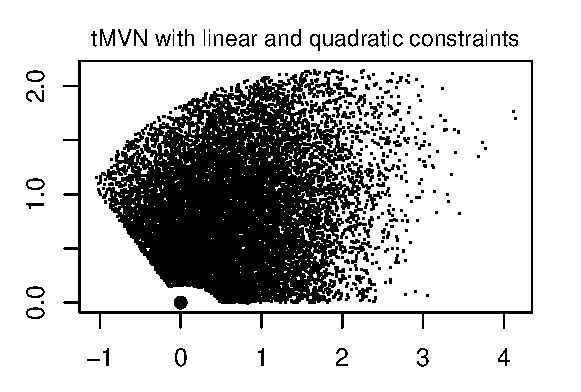
\includegraphics[scale=0.76]{tmvn_linear_quadratic_constr.eps}
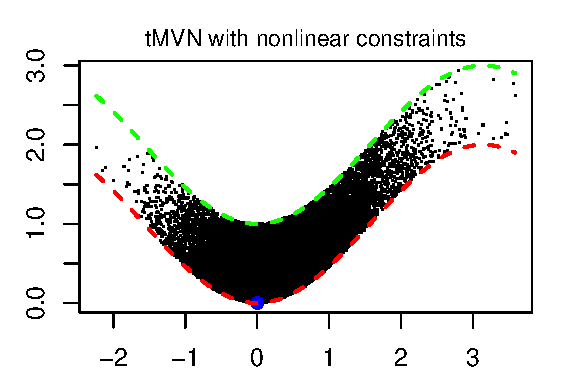
\includegraphics[scale=0.76]{tmvn_nonlinear_constr.eps}
\caption{Sampling 15,000 McMC samples from a bivariate Gaussian vector subject to linear and quadratic constraints (left panel), and to nonlinear constraints (right panel).}
\label{fig:tmvn}
\end{figure}





%\medskip
\section*{References}
\begin{enumerate}
	\item[{[1]}] Maatouk, Hassan \& Xavier Bay (2017). {\it Gaussian process emulators for computer experiments with inequality constraints}. Mathematical Geosciences 49(5):557-582.
	\item[{[2]}] Murray, Iain \& Ryan Prescott Adams \&  David J.C. MacKay (2010). {\it Elliptical slice sampling}. In: Proceedings of the thirteenth international conference on artificial intelligence and statistics, JMLR Workshop and Conference Proceedings, pp 541-548.
	\item[{[3]}] Pakman, Ari \& Liam Paninski (2014). {\it Exact Hamiltonian Monte Carlo for truncated multivariate Gaussians}. Journal of Computational and Graphical Statistics 23(2):518-542.
\end{enumerate}

\end{talk}

\begin{talk}
  {Copula-Based Regression with Discrete Covariates}% [1] talk title
  {Othmane Kortbi}% [2] speaker name
  {Department of Statistics and Business Analytics, UAE University, UAE}% [3] affiliations
  {okortbi@uaeu.ac.ae}% [4] email
  {} % [5] coauthors
{}{\timeslot{Thursday, August 22, 2024 -- Afternoon}{STC 0060}}{CS9-3}{CS9}

				% Insert the title of the special session if you were invited to give a talk in a special session.

In this project we investigated a new approach of estimating a regression function
based on copulas when covariates are mixture of continuous and discrete variables,
which is considered as an extension of Noh et al (2013) context. 
The main idea behind this approach is the writing of the regression function in terms of copula and marginal distributions,
thereafter we estimated the copula and marginal distributions. Now, since various 
methods are available in the literature to estimate both the copula and the marginals, this
approach offered us a rich and 
flexible alternative to many existing regression estimators.
We have studied the asymptotic behavior of the estimators obtained as well as the finite
sample performance of the estimators and illustrated their usefulness by analyzing real
data. An adapted algorithm is applied to construct copulas. Monte Carlo simulations are carried out 
to replicate datasets, estimate prediction model parameters and validate them.
 
\medskip


\begin{enumerate}

	
	\item[{[1]}] Crawley, M.J. (2005). {\it Statistics: An Introduction using R}. John Wiley \& Sons, Ltd.
	
	\item[{[2]}]Nelsen, R. B. (2006). {\it An introduction to copulas}. Springer Series in Statistics. Springer, New York.
	
	\item[{[3]}] Noh, H., Ghouch, A. E., and Bouezmarni, T. (2013). {\it Copula-based regression estimation and inference}. Journal of the American Statistical Association, 108(502), 676-688.
	
	\item[{[4]}] C. Ritz, C. and Streibig, J.C. (2008). {\it Nonlinear Regression in R}. Springer.

\item[{[5]}] Yan, J. (2007). {\it Enjoy the Joy of Copulas : With a Package copula}. Journal of Statistical Software, 21.

\end{enumerate}

\end{talk}

\begin{talk}
  {Geometric unification of central MCMC algorithms via rate distortion theory and factorizability of multivariate Markov chains}% [1] talk title
  {Michael Choi}% [2] speaker name
  {Department of Statistics and Data Science, National University of Singapore}% [3] affiliations
  {mchchoi@nus.edu.sg}% [4] email
  {Youjia Wang, Geoffrey Wolfer}% [5] coauthors
{}{\timeslot{Friday, August 23, 2024 -- Morning}{STC 0020}}{SS1-1}{SS1}

				% Insert the title of the special session if you were invited to give a talk in a special session.

Motivated by the notion of mutual information between two random variables and rate distortion theory, we propose and analyze a rate distortion optimization problem for Markov chains based upon information divergences between transition matrices. This framework offers a unified variational view on the optimality of a comprehensive suite of MCMC algorithms such as Metropolis-Hastings, Glauber dynamics, swapping algorithm and Feynman-Kac path models. Along the way, we put forward an alternative notion of distance to independence, or more generally factorizability, of a given Markov chain on a finite product state space, which is of independent interest. We prove a counterpart of the Shearer's lemma governing the distance to independence and entropy rate of Markov chains and their information projections. In addition, we develop mixing and hitting time comparison results between the original chain and its information projections, as well as a Sanov's theorem in this context. These considerations eventually lead us to investigate the geometry of multivariate Markov chains induced by information divergences.
\end{talk}

\begin{talk}
  {A large deviation principle for Metropolis-Hastings sampling}% [1] talk title
  {Federica Milinanni}% [2] speaker name
  {KTH Royal Institute of Technology, Sweden}% [3] affiliations
  {fedmil@kth.se}% [4] email
  {Pierre Nyquist}% [5] coauthors
{}{\timeslot{Friday, August 23, 2024 -- Morning}{STC 0020}}{SS1-2}{SS1}

				% Insert the title of the special session if you were invited to give a talk in a special session.
			
Sampling algorithms from the class of Markov chain Monte Carlo (MCMC) methods are widely used across scientific disciplines. Good performance measures are essential to analyse these methods, to compare different MCMC algorithms, and to tune parameters within a given method. Common tools that are used for analysing convergence properties of MCMC algorithms are, e.g., mixing times, spectral gap and functional inequalities (e.g. Poincaré, log-Sobolev). A further, rather novel, approach consists in the use of large deviations theory to study the convergence of empirical measures of MCMC chains. At the heart of large deviations theory is the large deviation principle, which allows us to describe the rate of convergence of the empirical measures through a so-called rate function.

In this talk we will consider Markov chains generated via MCMC methods of Metropolis-Hastings type for sampling from a target distribution on a Polish space. We will state a large deviation principle for the corresponding empirical measure, show examples of algorithms from this class for which the theorem applies, and illustrate how the result can be used to tune algorithms' parameters.

\medskip

\begin{enumerate}
	\item[{[1]}] Milinanni, F., \& Nyquist, P. (2024). A large deviation principle for the empirical measures of Metropolis–Hastings chains. \textit{Stochastic Processes and their Applications, 170}, 104293.
	\item[{[2]}] Milinanni, F., \& Nyquist, P. (2024). On the large deviation principle for Metropolis-Hastings Markov Chains: the Lyapunov function condition and examples. \textit{arXiv preprint arXiv:2403.08691.}
\end{enumerate}


\end{talk}

\begin{talk}
  {On the Convergence of MCMCs with Quantum Speedup}% [1] talk title
  {Ning Ning}% [2] speaker name
  {Texas A\&M University, College Station}% [3] affiliations
  {patning@tamu.edu}% [4] email
  {}% [5] coauthors
{}{\timeslot{Friday, August 23, 2024 -- Morning}{STC 0020}}{SS1-3}{SS1}

				% Insert the title of the special session if you were invited to give a talk in a special session.

				
				

Quantum computing has emerged as a promising avenue for accelerating various computational tasks, including optimization and sampling problems. One particularly intriguing application lies in the realm of Markov Chain Monte Carlo (MCMC) algorithms, fundamental tools widely used in Bayesian inference, statistical physics, and machine learning. This talk delves into the convergence properties of MCMCs enhanced with quantum speedup. We investigate how quantum computing techniques can potentially expedite the convergence of MCMC algorithms, leading to more efficient sampling from complex probability distributions. 
%Our analysis encompasses theoretical frameworks and practical considerations, shedding light on the interplay between quantum mechanics and stochastic processes. 
We explore key theoretical concepts underlying quantum-enhanced MCMCs, examining the impact of quantum resources on convergence rates and sampling quality.
\end{talk}

\begin{talk}
  {Adapting the Stereographic Bouncy Particle Sampler}% [1] talk title
  {Cameron Bell}% [2] speaker name
  {University of Warwick, UK}% [3] affiliations
  {cameron.bell@warwick.ac.uk}% [4] email
  {Krzysztof {\L}atuszy{\'n}ski and Gareth O. Roberts}% [5] coauthors
{}{\timeslot{Friday, August 23, 2024 -- Morning}{STC 0020}}{SS1-4}{SS1}

				% Insert the title of the special session if you were invited to give a talk in a special session.
			

In order to tackle the problem of sampling from heavy tailed, high dimensional distributions via Markov Chain Monte Carlo (MCMC) methods, Yang, {\L}atuszy{\'n}ski and Roberts (2022) introduces the stereographic projection as a tool to compactify $\mathbb{R}^d$ and transform the problem into sampling from a density on the unit sphere $\mathbb{S}^d$. The MCMC algorithms (a random walk Metropolis algorithm and a bouncy particle sampler) presented in that paper are shown to be uniformly ergodic, even for certain polynomial-tailed target distributions, where Euclidean MCMC algorithms result in chains that are not even geometrically ergodic. Furthermore, robustness properties are provided to show that these stereographic MCMC algorithms perform at least as well as their Euclidean counterparts in terms of asymptotic variance of estimator. In the best case scenario, they exhibit a ``blessing of dimensionality" which allows them to return to the high probability region faster as the dimension increases. However, the improvement in algorithmic efficiency, as well as the computational cost of the implementation, are still significantly impacted by the parameters used in this transformation (which provide an affine preconditioning of $\mathbb{R}^d$).

We introduce an adaptive version of the Stereographic Bouncy Particle Sampler (SBPS) which automatically updates the parameters of the algorithm as the run progresses. The adaptive setup allows us to better exploit the power of the stereographic projection, even when the initial parameters are poorly chosen.

Leveraging the simultaneous uniform ergodicity of the SBPS and the Adapting Increasingly Rarely framework (Chimisov, {\L}atuszy{\'n}ski and Roberts (2018)), we establish a novel framework for proving convergence of continuous time adaptive MCMC algorithms which allow us to prove LLNs and a CLT for the adaptive SBPS. We demonstrate the ability of the adaptive SBPS algorithm in several simulation studies, such as estimating tail probabilities of heavy tailed, high dimensional target distributions, which show that it can outperform algorithms such as HMC in these settings.

\begin{enumerate}
	\item[{[1]}] Yang, Jun, {\L}atuszy{\'n}ski, Krzysztof and Roberts, Gareth O. (2022). {\it Stereographic Markov Chain Monte Carlo}. arXiv preprint arXiv:2205.12112.
	\item[{[2]}] Chimisov, Cyril, {\L}atuszy{\'n}ski, Krzysztof and Roberts, Gareth O. (2018). {\it Air Markov chain Monte Carlo}. arXiv preprint arXiv:1801.09309.
\end{enumerate}
\end{talk}

\begin{talk}
  {Losing momentum in continuous-time stochastic optimisation}% [1] talk title
  {Jonas Latz}% [2] speaker name
  {University of Manchester}% [3] affiliations
  {jonas.latz@manchester.ac.uk}% [4] email
  {Kexin Jin, Chenguang Liu, Alessandro Scagliotti}% [5] coauthors
{}{\timeslot{Friday, August 23, 2024 -- Morning}{STC 0040}}{SS17-1}{SS17}

				% Insert the title of the special session if you were invited to give a talk in a special session.
			
The training of deep neural networks and other modern machine learning models usually consists in solving non-convex optimisation problems that are high-dimensional and subject to large-scale data. Here, momentum-based stochastic optimisation algorithms have become especially popular in recent years. The stochasticity arises from data subsampling which reduces computational cost. Moreover, both, momentum and stochasticity are supposed to help the algorithm to overcome local minimisers and, hopefully, converge globally. Theoretically, this combination of stochasticity and momentum is badly understood.

In our work [1], we propose and analyse a continuous-time model for stochastic gradient descent with momentum. This model is a piecewise-deterministic Markov process that represents the particle movement by an underdamped dynamical system and the data subsampling through a stochastic switching of the dynamical system. In our analysis, we investigate longtime limits, the subsampling-to-no-subsampling limit, and the momentum-to-no-momentum limit. We are particularly interested in the case of reducing the momentum over time: intuitively, the momentum helps to overcome local minimisers in the initial phase of the algorithm, but prohibits fast convergence to a global minimiser later. Under convexity assumptions, we show convergence of our dynamical system to the global minimiser when reducing momentum over time and let the subsampling rate go to infinity.

We then propose a stable, symplectic discretisation scheme to construct an algorithm from our continuous-time dynamical system. In numerical experiments, we study our discretisation scheme in convex and non-convex test problems. Additionally, we train a convolutional neural network to solve the CIFAR-10 image classification problem. Here, our algorithm reaches competitive results compared to stochastic gradient descent with momentum.

\medskip

\begin{enumerate}
	\item[{[1]}] Jin, Kexin, Jonas Latz, Chenguang Liu, \& Alessandro Scagliotti (2022). Losing momentum in continuous-time stochastic optimisation. arXiv:2209.03705.
\end{enumerate}

\end{talk}

\begin{talk}
  {How to choose an annealing algorithm}% [1] talk title
  {Alexandre Bouchard-C\^ot\'e}% [2] speaker name
  {University of British Columbia}% [3] affiliations
  {bouchard@stat.ubc.ca}% [4] email
  {Saifuddin Syed, Kevin Chern, Arnaud Doucet}% [5] coauthors
{}{\timeslot{Friday, August 23, 2024 -- Morning}{STC 0040}}{SS17-2}{SS17}

				% Insert the title of the special session if you were invited to give a talk in a special session.

				
				

Over the years, several algorithms have been developed to tackle normalization constant estimation. A handful of those have passed the test of time thanks to their capacity to beat the curse of dimensionality in many realistic scenarios: on one hand, Annealed Importance Sampling (AIS) and Sequential Monte Carlo (SMC) methods, and on the other, Parallel Tempering (PT) and Simulated Tempering (ST) algorithms. Indeed many recent developments can be contextualized as members of one of these two families of meta-algorithms.

A priori, these two families of algorithms, AIS/SMC versus PT/ST, appear quite distinct and indeed these communities are largely silos. This leads to an important practical question: for a given problem, which annealing algorithm should be recommended? I will present our work toward tackling this question, in which a key object needed for theoretical and methodological purposes is the rate function of various limiting PDMPs. 
\end{talk}

\begin{talk}
  {Projected ensemble data assimilation}% [1] talk title
  {S. B. Dubinkina }% [2] speaker name
  {Amsterdam Center for Dynamics and Computation, the Department of Mathematics, VU Amsterdam, The Netherlands}% [3] affiliations
  {s.b.dubinkina@vu.nl}% [4] email
  {J. de Wiljes}% [5] coauthors
{}{\timeslot{Friday, August 23, 2024 -- Morning}{STC 0040}}{SS17-3}{SS17}

				% Insert the title of the special session if you were invited to give a talk in a special session.
			
Ensemble data assimilation is unable to reduce the error estimate for high-dimensional systems when used with small ensemble size. A typical remedy is dimesion reduction by localization. Though localization reduces the error substantially for both linear and nonlinear data-assimilation methods, the former ones considerably outperform the latter ones in a quasi-linear regime. We propose a further dimension reduction based on projection and show substantial error decrease of a nonlinear data-assimilation method in a challenging data-assimilation setup with small ensemble size and ample observations.  

\medskip

\end{talk}

\begin{talk}
{Approximation of vectors using adaptive randomized information}
{Marcin Wnuk}
{Osnabr\"uck University}
{marcin.wnuk@uni-osnabrueck.de}
{Robert J. Kunsch}
{}{\timeslot{Friday, August 23, 2024 -- Morning}{STC 0040}}{SS17-4}{SS17}



Working in the framework of Information-Based Complexity we study approximation of the embedding $\ell_p^m \hookrightarrow \ell_q^m$, $1 \leq p < q \leq \infty$,
based on randomized adaptive algorithms that use arbitrary linear 
functionals as information on a problem instance.
In the case $p \leq 2$ and $q = \infty$
we show upper bounds for which the complexity $n$ 
exhibits only a $(\log\log m)$-dependence. 
In particular we improve upon known results for $p=1$ and $q=\infty$
and by this give an example for a gap of order $n / (\log n)^2$
for the error for adaptive vs.\ non-adaptive Monte Carlo methods
which is the biggest possible gap for linear problems up to logarithmic factors.

\end{talk}

\begin{talk}
  {Function space embeddings for non-tensor product spaces and application to high-dimensional approximation}% [1] talk title
  {Michael Gnewuch}% [2] speaker name
  {University of Osnabr\"uck}% [3] affiliations
  {michael.gnewuch@uos.de}% [4] email
  {Peter Kritzer, Klaus Ritter}% [5] coauthors
{}{\timeslot{Friday, August 23, 2024 -- Morning}{STC 0050}}{SS24-1}{SS24}

				% Insert the title of the special session if you were invited to give a talk in a special session.
			
%Your abstract goes here. Please do not use your own commands or macros.
%Embeddings of (scales of) function spaces are helpful tools to transfer the analysis of algorithms from 


%In this talk we want to discuss a general approach 

%In the analysis of high-dimensional problems 

In tractability analysis one is interested in continuous approximation problems
that are defined on a scale of function spaces $(H_d)_{d\in {\mathbb N}}$, where the parameter
$d$ typically denotes the number of variables the functions in $H_d$ depend on.
An important goal is to find algorithms that scale well with respect to the dimension parameter $d$ and help to break the curse of dimensionality. 
Some specific features of the function spaces can be very helpful for the analysis of certain types of algorithms; e.g., for the analysis of unbiased randomized algorithms it may be extremely helpful if the norm on $H_d$ induces an ANOVA decomposition on $H_d$, which can be used to analyze the error ($=$ variance) of the algorithms. 
In general, a suitable embedding of scales of function spaces may help to transfer results from scales of function spaces with favourable features to other scales of interest. There are several general embedding results known in the case where $H_d$ is the $d$-fold tensor product of a reproducing kernel Hilbert space (RKHS) 
$H_1$; examples include weighted RKHSs where the weights are product weights and so-called spaces of increasing smoothness.
%, cf., e.g., [1] and [2]. 

In this talk we discuss a general embedding approach that still works in the case where $H_d$ is not necessarily of tensor product form. This is, e.g., the case if we consider weighted RKHSs, where the weights are product and order-dependent weights or finite-order weights. As an application we study $L^\infty$-approximation on a RKHS of functions that depend on infinitely many variables (which can be viewed as a limiting case of tractability analysis).



\medskip

%If you would like to include references, please do so by creating a simple list numbered by [1], [2], [3], \ldots. See example below.
%Please do not use the \texttt{bibliography} environment or \texttt{bibtex} files.
%APA reference style is recommended.

%\begin{enumerate}
%	\item[{[1]}] M. Gnewuch, M. Hefter, A. Hinrichs, and K. Ritter. Embeddings of %weighted Hilbert spaces and applications to multivariate and infinite-dimensional %integration, J. Approx. Theory, 222 (2017), 8--39. 
%	\item[{[2]}] M. Gnewuch, M. Hefter, A. Hinrichs, K. Ritter, and G. W. Wasilkowski. Embeddings for  infinite-dimensional integration and $L_2$-approximation with increasing smoothness, J. Complexity, 54 (2019), 101406, 1--32. 
%\end{enumerate}

%Equations may be used if they are referenced. Please note that the equation numbers may be different (but will be cross-referenced correctly) in the final program book.
\end{talk}

\begin{talk}
  {ANOVA-boosting for high-dimensional approximation}% [1] talk title
  {Laura Weidensager}% [2] speaker name
  {Chemnitz University of Technology}% [3] affiliations
  {laura.weidensager@math.tu-chemnitz.de}% [4] email
  {Daniel Potts}% [5] coauthors
{}{\timeslot{Friday, August 23, 2024 -- Morning}{STC 0050}}{SS24-2}{SS24}

				% Insert the title of the special session if you were invited to give a talk in a special session.

				
				
We study the problem of scattered-data approximation on $\mathbb{R}^d$, where we have given sample points and the corresponding function evaluations of a function $f$. The random Fourier feature approach is a two-layer network with a randomized but fixed single hidden layer. The output layer is trained. In this talk we present algorithms from [1], which aim to adapt the randomized hidden layer to the function $f$.\par
We use the analysis of variance (ANOVA) decomposition 
$$f(\mathbf{ x}) = \sum_{\mathbf{ u}\subseteq \{1,\ldots, d\}} f_{\mathbf{ u}}(\mathbf{ x}_{\mathbf{\mathbf{ u}}})$$
for approximating high-dimensional functions of low effective dimension. Thereby we give a relation between the Fourier transform of the function $f$ and the ANOVA terms $f_{\mathbf{u}}$. \par
In the case for dependent input variables, the ANOVA decomposition is generalized with the aim to detect the structure of the function. We use a least-squares algorithm with a regularization which penalizes the non-orthogonality of ANOVA terms to find which input variables and variable interactions are important. This information is then used to boost random Fourier feature algorithms. 

\medskip

[1] Potts, D., Weidensager, L. ANOVA-boosting for Random Fourier Features, \textit{ArXiv e-print: 2404.03050}, 2024\\
\end{talk}

\begin{talk}
  {Tractability results for integration on Gaussian spaces}% [1] talk title
  {Robin Rüßmann}% [2] speaker name
  {RPTU Kaiserslautern}% [3] affiliations
  {ruessmann@mathematik.uni-kl.de}% [4] email
  {Michael Gnewuch, Klaus Ritter}% [5] coauthors
{}{\timeslot{Friday, August 23, 2024 -- Morning}{STC 0050}}{SS24-3}{SS24}

				% Insert the title of the special session if you were invited to give a talk in a special session.
			
We study integration with respect to the $d$-dimensional standard normal distribution on Gaussian spaces. Here, given shape parameters $\sigma_j>0$, a Gaussian space is a reproducing kernel Hilbert space, whose kernel is defined by $L_{\boldsymbol{\sigma}}(x,y)=\prod_{j=1}^d \exp(-\sigma_j^2(x_j-y_j)^2)$.  

We give new tractability results based on the asymptotic behavior of $\sigma_j$ as $j$ tends to infinity. Positive results are obtained both from previously established algorithms, as well as a new transference principle between Gaussian spaces and Hermite spaces.   

\end{talk}

\begin{talk}
  {Unbiased and Multilevel Methods for a Class of Diffusions Partially Observed via Marked Point Processes}% [1] talk title
  {Miguel Alvarez}% [2] speaker name
  {King Abdullah University of Science and Technology (KAUST)}% [3] affiliations
  {miguelangel.alvarezballesteros@kaust.edu.sa}% [4] email
  {Ajay Jasra, Hamza Ruzayqat}% [5] coauthors
{}{\timeslot{Friday, August 23, 2024 -- Morning}{STC 0060}}{CS11-1}{CS11}

				% Insert the title of the special session if you were invited to give a talk in a special session.
			
In this talk we consider the filtering problem associated to partially observed diffusions, with observations following a marked point process.
In the model, the data form a point process with observation times that have its intensity driven by a diffusion, with the associated marks also depending upon the diffusion process.
We assume that one must resort to time-discretizing the diffusion process and develop particle and multilevel particle filters to recursively approximate the filter.
In particular, we prove that our multilevel particle filter can achieve a mean square error (MSE) of $\mathcal{O}(\epsilon^2)$ ($\epsilon>0$ and arbitrary) with a cost
of $\mathcal{O}(\epsilon^{-2.5})$ versus using a particle filter which has a cost of $\mathcal{O}(\epsilon^{-3})$ to achieve the same MSE. We then show how this methodology can be extended to give unbiased (that is with no time-discretization error) estimators of the filter, which are proved to have finite variance and with high-probability have finite cost. Finally, we extend our methodology to the problem of online static-parameter estimation.

\medskip

\end{talk}

\begin{talk}
 {Multilevel optimization-based sampling for large-scale inverse problems}% [1] talk title
  {Chuntao Chen}% [2] speaker name
  {Lappeenranta University of Technology}% [3] affiliations
  {Chuntao.Chen@lut.fi}% [4] email
  {Tiangang Cui, Youssef Marzouk}% [5] coauthors
{}{\timeslot{Friday, August 23, 2024 -- Morning}{STC 0060}}{CS11-2}{CS11}

				% Insert the title of the special session if you were invited to give a talk in a special session.
			
We combine the Multilevel Monte Carlo and the optimization-based samplers, including Randomized-and-Then-Optimize (RTO) and Implicit Sampling, to address the challenges that classical MCMC faces, and implements the samplers in computationally costly Bayesian inverse problems including an ODE model and a PDE problem. Simulations using the optimization-based samplers like RTO can be parallelized which allows us to develop efficient
MCMC algorithms or self-normalizing estimators to solve the inverse problems. Multilevel Monte Carlo is proven to significantly reduce the computational cost of Monte Carlo simu-
lation, which helps us further improve the RTO method. To adapt the multilevel method on the optimization-based samplers, we develop the complexity theorem for multilevel self-normalizing estimators. The corresponding numerical experiments produce good results on RTO method, showing a high effective sample ratio in the importance sampling scheme, and the variances of the self-normalizing estimators converge when discretization size decreases.


\medskip




\end{talk}

\begin{talk}
  {Single-ensemble multilevel Monte Carlo for discrete interacting-particle methods}% [1] talk title
  {Arne Bouillon}% [2] speaker name
  {KU Leuven}% [3] affiliations
  {arne.bouillon@kuleuven.be}% [4] email
  {Toon Ingelaere, Giovanni Samaey}% [5] coauthors
{}{\timeslot{Friday, August 23, 2024 -- Morning}{STC 0060}}{CS11-3}{CS11}

				% Insert the title of the special session if you were invited to give a talk in a special session.

Interacting-particle methods have found applications in domains such as filtering, optimization and posterior sampling. These parallelizable and often gradient-free algorithms use an ensemble of particles that evolve in time, based on the combination of well-chosen dynamics and interaction between the particles. For computationally expensive dynamics -- for example, Bayesian inversion with an expensive forward model or optimization of an expensive objective function -- the cost of attaining a high accuracy quickly becomes prohibitive.

In this talk, we discuss our recent work [1], in which we exploit a hierarchy of approximations to this forward model and apply multilevel Monte Carlo (MLMC) techniques. More specifically, we extend the approach suggested in [2, 3] for the ensemble Kalman filter: we use MLMC at each time step to estimate the interaction term within a single, globally-coupled ensemble. We formulate conditions on the method dynamics, interaction term, and forward model, under which we prove an asymptotic bound on the cost-to-error relation. This bound suggests that a multilevel simulation strategy is more efficient than a single-level one for a large family of interacting-particle methods. Numerical experiments corroborate our analysis of the improved asymptotic cost-to-error rate.

\medskip

[1] A. Bouillon, T. Ingelaere, G. Samaey, Single-ensemble multilevel Monte Carlo for discrete interacting-particle methods, in preparation.

[2] H. Hoel, K. J. H. Law, and R. Tempone, Multilevel ensemble Kalman filtering, SIAM J. Numer. Anal., 54 (2016), pp.\ 1813--1839.

[3] A. Chernov, H. Hoel, K. J. H. Law, F. Nobile, and R. Tempone, Multilevel ensemble Kalman filtering for spatio-temporal processes, Numer. Math., 147 (2021), pp.\ 71--125.
\end{talk}

